\chapter{Data Analysis}
\label{ch:analysis}

This chapter presents the full analysis strategy for the search for the charged Higgs boson in rare top quark decays. The collision data and simulated samples are described in Section~\ref{sec:datasets}, followed by the reconstruction and identification of physics objects in Section~\ref{sec:objects}. The signal extraction strategy, including the baseline event selection, the ParticleNet-based multivariate approach, and the template construction and statistical framework, is detailed in Section~\ref{sec:signal_extraction}. The estimation of Standard Model backgrounds is presented in Section~\ref{sec:background}, the treatment of systematic uncertainties is discussed in Section~\ref{sec:systematics}, and the results are presented in Section~\ref{sec:results}.

%% ============================================================
\section{Datasets and Triggers}
\label{sec:datasets}
%% ============================================================

\subsection{Collision data}
\label{ssec:collision_data}

The analysis uses proton-proton ($\Pp\Pp$) collision data collected by the CMS experiment during LHC Run~2 (2016--2018) at a center-of-mass energy of $\sqrt{s} = 13\TeV$ and Run~3 (2022--2023) at $\sqrt{s} = 13.6\TeV$. Good quality events in which all detector subsystems are flagged as fully operational are selected using certified luminosity sections provided by the CMS data quality monitoring group. The integrated luminosity for each data-taking period is summarized in Table~\ref{tab:luminosity}.

\begin{table}[htbp]
\centering
\caption{Integrated luminosity for each data-taking period used in the analysis.}
\label{tab:luminosity}
\begin{tabular}{llc}
\hline\hline
Run period & Era & Integrated luminosity (\fbinv) \\
\hline
\multirow{4}{*}{Run~2 (13\TeV)}
 & 2016 preVFP  & 19.5 \\
 & 2016 postVFP & 16.8 \\
 & 2017         & 41.5 \\
 & 2018         & 59.8 \\
\hline
\multicolumn{2}{l}{Run~2 total} & 137.6 \\
\hline
\multirow{4}{*}{Run~3 (13.6\TeV)}
 & 2022         & 7.98 \\
 & 2022EE       & 26.7 \\
 & 2023         & 18.1 \\
 & 2023BPix     & 9.7 \\
\hline
\multicolumn{2}{l}{Run~3 total} & 62.5 \\
\hline
\multicolumn{2}{l}{\textbf{Combined total}} & \textbf{200.1} \\
\hline\hline
\end{tabular}
\end{table}

The 2016 data are divided into ``preVFP'' and ``postVFP'' periods, corresponding to data taken before and after changes to the silicon strip tracker front-end voltage regulation, which affected the tracking performance and required separate calibrations. For Run~3, the 2022 data are split at the boundary of era~F, where an update to the ECAL endcap conditions was introduced (``EE'' period), while the 2023 data are divided at the era~D boundary, where an inactive pixel barrel module (``BPix'' period) required dedicated calibration. The complete list of data samples is provided in Appendix~\ref{app:triggers}.

\subsection{Trigger strategy}
\label{ssec:triggers}

Events are collected using unprescaled dilepton triggers that provide high efficiency for the trilepton final states targeted by this analysis. The $\Pgm\Pgm\Pgm$ channel is selected using dimuon triggers, while the $\Pe\Pgm\Pgm$ channel uses electron-muon cross-triggers, with specific trigger paths varying across data-taking years to follow changes in the trigger menu. The complete list of trigger paths is provided in Appendix~\ref{app:triggers}.

In addition to the analysis triggers, prescaled single-lepton triggers are used to measure the fake rates for the nonprompt lepton background estimation described in Section~\ref{sec:background}, and unprescaled single-lepton triggers are used for lepton identification and trigger efficiency measurements.

\subsection{Monte Carlo simulation samples}
\label{ssec:mc_samples}

Monte Carlo (MC) simulated samples are used to model signal processes and prompt Standard Model (SM) backgrounds. The jet-induced nonprompt lepton background is estimated using a data-driven method, as described in Section~\ref{sec:background}, because the extremely low probability of jets producing leptons that pass identification criteria would require generating billions of events in processes such as $\ttbar$ and QCD multijet production to achieve adequate statistical precision.

The general simulation framework is described in Section~\ref{sec:mc_sim}. For the samples used in this analysis, hard-scattering matrix elements are computed with \MGvATNLO~\cite{MG5_aMCatNLO} or \POWHEG V2~\cite{Powheg1,Powheg2,Powheg3}, with parton shower and hadronization modeled by \PYTHIA 8~\cite{Pythia8} with the CP5 underlying event tune~\cite{CPTunes}. All samples use the NNPDF3.1 NNLO parton distribution function set~\cite{NNPDF31}. Simulated events are processed through the full \GEANTfour-based CMS detector simulation~\cite{Geant4}, and pileup interactions are reweighted to match the observed conditions in each data-taking period.

\subsubsection{Signal samples}

Signal MC samples for the process $\Pp\Pp \to \ttbar \to (\PHc\PQb)(\PW\PQb)$ with the subsequent decay $\PHc \to \PW^{(*)}\PA \to \PW^{(*)}\Pgmp\Pgmm$ are generated at leading order using the \MGvATNLO generator with the \texttt{2HDM\_UFO-type1\_5FS} model~\cite{FeynRules2HDM} in the five-flavor scheme. The decay of the top quark, $\PW$ boson, charged Higgs boson, and pseudoscalar is performed within the same generator, and all $\PW$ boson decay modes except fully hadronic decays are included. The top quark mass is set to $\mt = 172.5\GeV$, consistent with the SM samples. The widths of the hypothetical new bosons are set to 1~MeV following the narrow width approximation, consistent with the expected widths of $\mathcal{O}(\text{MeV})$ calculated by \textsc{2HDMC}~\cite{2HDMC}.

Signal samples are generated for a grid of $(\mHc, \mA)$ mass points listed in Table~\ref{tab:signal_masspoints}, covering the charged Higgs boson mass range $70 \leq \mHc \leq 160\GeV$ and pseudoscalar mass range $15\GeV \leq \mA \leq \mHc - 5\GeV$. This grid spans both the on-shell regime ($\mA < \mHc - \mW$), where the $\PW$ boson in the $\PHc$ decay is on its mass shell, and the off-shell regime ($\mA > \mHc - \mW$), where an off-shell $\PW^{*}$ is produced — a novel feature of this search not covered by previous analyses~\cite{CMSRun2ChargedHiggs}.

\begin{table}[htbp]
\centering
\caption{Signal mass points $(\mHc, \mA)$ in \GeVns used in the simulation.}
\label{tab:signal_masspoints}
\begin{tabular}{cl}
\hline\hline
$\mHc$ [\GeVns] & $\mA$ [\GeVns] \\
\hline
70  & 15, 18, 40, 55, 65 \\
85  & 15, 21, 70, 80 \\
100 & 15, 24, 60, 75, 95 \\
115 & 15, 27, 87, 110 \\
130 & 15, 30, 55, 83, 90, 100, 125 \\
145 & 15, 35, 92, 140 \\
160 & 15, 50, 85, 98, 120, 135, 155 \\
\hline\hline
\end{tabular}
\end{table}

The signal cross section is $\sigma_{\text{sig}} = 2 \times \sigma_{\ttbar} \times \mathcal{B}_{\text{cascade}}$ (Eq.~\ref{eq:cascade_BR}), with $\ttbar$ production cross sections of 833.9~pb and 923.6~pb at $\sqrt{s} = 13$ and 13.6\TeV respectively, computed at NNLO+NNLL accuracy~\cite{TTbarXsecRecommedation}.

\subsubsection{Background samples}

The SM backgrounds that produce three or more prompt leptons constitute the irreducible backgrounds to this search. The dominant contribution arises from $\PW\PZ$ production where both bosons decay leptonically, followed by $\PZ\PZ \to 4\ell$ where one lepton escapes detection. Smaller contributions come from $\ttbar$ production in association with a $\PW$, $\PZ$, or Higgs boson, single top quark production with a $\PZ$ boson ($\cPqt\PZ\cPq$), triboson processes ($\PW\PW\PW$, $\PW\PW\PZ$, $\PW\PZ\PZ$, $\PZ\PZ\PZ$), and SM Higgs boson production through gluon fusion, vector boson fusion, and associated production.

The conversion background arises from events in which a prompt photon converts into a lepton pair, either externally through interaction with detector material or internally through the virtual photon process $\gamma^{*} \to \ell^{+}\ell^{-}$ in QED shower evolution. The relevant processes are Drell--Yan production with an associated photon ($\PZ\gamma$) and $\ttbar\gamma$ production, both simulated at NLO with the \MGvATNLO generator. A conversion electron is identified at the generator level as a reconstructed electron that does not match a generator-level final state electron within $\Delta R < 0.1$, but matches a generator-level prompt photon with $\Delta\pT/\pT < 0.5$ and $\Delta R < 0.2$ whose origin does not trace back to a hadron. The virtuality of the photons producing internal conversions is limited to $(4\GeV)^{2}$, ensuring no overlap with the $\PW\PZ$, $\PZ\PZ$, $\ttbar\PZ$, and $\cPqt\PZ$ samples.

Additional MC samples are used for control region studies: Drell--Yan and $\ttbar$ samples for validation of the nonprompt lepton estimation, single top production in various channels for dilepton control regions, and high-statistics $\PZ \to \ell\ell$ samples generated at NNLO with \POWHEG MiNNLO~\cite{PowhegMiNNLO_Z1,PowhegMiNNLO_Z2} for precise lepton efficiency measurements.

Generator-level cross sections are corrected to higher-order theoretical predictions as summarized in Table~\ref{tab:mc_summary}. The complete sample lists are given in Appendix~\ref{app:mc_samples}.

\begin{table}[htbp]
\centering
\caption{Summary of MC samples used in the analysis. Cross sections are given as $\sigma\mathcal{B}$ at 13\TeV / 13.6\TeV. Samples are generated with \MGvATNLO or \POWHEG V2; complete sample lists are given in Appendix~\ref{app:mc_samples}.}
\label{tab:mc_summary}
\small
\begin{tabular}{p{4.2cm}p{3.2cm}l}
\hline\hline
Process & $\sigma\mathcal{B}$ [pb] & Order \\
\hline
\multicolumn{3}{l}{\textit{Prompt trilepton}} \\
$\PW\PZ \to 3\ell\Pgn$     & 5.78 / 5.85   & NNLO QCD \\
$\PZ\PZ \to 4\ell$          & 1.46 / 1.77   & NNLO QCD \\
$\ttbar\PW$                  & 0.235 / 0.288 & aN$^{3}$LO QCD \\
$\ttbar\PZ$                  & 0.294 / 0.146 & aN$^{3}$LO + NLO EW \\
$\ttbar\PH$                  & 0.215 / 0.241 & NLO + NLO EW \\
$\cPqt\PZ\cPq$              & 0.076 / 0.080 & NLO QCD \\
Tribosons                    & 0.443 / 0.496 & NLO \\
\hline
\multicolumn{3}{l}{\textit{Conversion}} \\
$\PZ\gamma$ (DY)             & $\sim$6080 / $\sim$6350 & NNLO \\
$\ttbar\gamma$               & 3.76 / 4.76   & NLO \\
\hline
\multicolumn{3}{l}{\textit{Control region}} \\
$\ttbar$                     & 833.9 / 923.6 & NNLO+NNLL \\
Single top ($\cPqt\PW$, s, t-ch.) & various & $\sim$NNLO \\
$\PW\PW$, $\PW\PZ$, $\PZ\PZ$ (inclusive) & various & NNLO QCD $\times$ NLO EW \\
\hline\hline
\end{tabular}
\end{table}



%% ============================================================
\section{Object Definitions}
\label{sec:objects}
%% ============================================================

The physics objects used in this analysis --- electrons, muons, jets, and missing transverse momentum --- are reconstructed from the particle-flow (PF) candidates described in Section~\ref{sec:pf}. This section defines the analysis-specific identification criteria and kinematic selections applied to each object type. Two working points are defined for leptons: a \textit{tight} working point used to select signal candidates, and a \textit{loose} working point that relaxes the isolation and impact parameter requirements to define sidebands for the data-driven nonprompt lepton background estimation described in Section~\ref{sec:background}.

\subsection{Electrons}
\label{ssec:electrons}

Electron candidates are required to have $\pT > 15\GeV$ and $|\eta| < 2.5$, excluding the barrel--endcap transition region $1.442 < |\eta| < 1.566$ where reconstruction quality degrades. The $\pT$ threshold is driven by the dilepton trigger acceptance described in Section~\ref{ssec:triggers}. In the 2018 data, electron candidates in the region $\eta_\text{SC} < -1.3$ and $-1.57 < \phi_\text{SC} < -0.87$ are vetoed due to the HEM 15/16 failure in the HCAL endcap~\cite{CMS-DP-2020-015}.

Electron identification uses the multivariate (MVA) discriminant provided by the EGM POG, which combines track quality and electromagnetic shower shape variables in a boosted decision tree trained separately in three pseudorapidity regions. The tight working point uses the POG wp90 selection, corresponding to approximately 90\% prompt electron identification efficiency. The identification is complemented by requirements on the significance of the three-dimensional impact parameter ($|\text{SIP3D}| < 4$) and a conversion veto with at most one expected missing inner tracker hit, which suppress electrons from photon conversions and secondary vertices.

Isolation is evaluated using the mini-isolation variable (Section~\ref{sec:pf}), which employs a $\pT$-dependent cone radius:
\begin{equation}
\label{eq:miniiso_cone}
\Delta R = \begin{cases} 0.2 & \pT < 50\GeV \\ 10\GeV / \pT & 50 \leq \pT < 200\GeV \\ 0.05 & \pT \geq 200\GeV \end{cases}
\end{equation}
The tight working point requires $I_\text{mini} < 0.1$, yielding approximately 90\% efficiency for prompt electrons and 15\% for nonprompt electrons from heavy-flavor decays. Additional cuts on shower shape and calorimeter variables are applied to emulate the online trigger reconstruction, ensuring that the offline selection remains fully efficient with respect to the trigger.

The loose working point relaxes the MVA discriminant threshold, isolation ($I_\text{mini} < 0.4$), and impact parameter ($|\text{SIP3D}| < 8$) requirements to define an enlarged sample enriched in nonprompt leptons. The complete selection criteria for both working points are summarized in Table~\ref{tab:electron_id}.

\begin{table}[htbp]
\centering
\caption{Electron identification criteria for the tight and loose working points. Values in parentheses denote $\eta$-dependent thresholds for the barrel/endcap regions split at $|\eta| = 1.479$, or for three regions at $|\eta| = 0.8$ and $1.479$.}
\label{tab:electron_id}
\small
\begin{tabular}{lccc}
\hline\hline
Variable & Tight WP & Loose WP (Run~2) & Loose WP (Run~3) \\
\hline
MVANoIso & POG wp90 & $>(0.985, 0.96, 0.85)$ & $>(0.8, 0.5, -0.8)$ \\
$I_\text{mini}$ & $<0.1$ & $<0.4$ & $<0.4$ \\
$|\text{SIP3D}|$ & $<4$ & $<8$ & $<8$ \\
Missing inner hits & $\leq 1$ & $\leq 1$ & $\leq 1$ \\
Conversion veto & yes & yes & yes \\
HLT emulation & \checkmark & \checkmark & \checkmark \\
\hline\hline
\end{tabular}
\end{table}

\subsection{Muons}
\label{ssec:muons}

Muon candidates are required to have $\pT > 10\GeV$ and $|\eta| < 2.4$, corresponding to the full coverage of the muon system. The lower $\pT$ threshold compared to electrons reflects the cleaner muon signature and the dimuon trigger acceptance for the subleading leg.

Muon identification uses the POG medium working point, which requires a high-quality track with few kinks, a large fraction of compatible muon chamber segments, and a consistent combined fit of the tracker and muon system tracks. Muon momentum is corrected using the Rochester correction procedure~\cite{Rochester}, which calibrates the muon momentum scale and resolution using $\PZ \to \Pgmp\Pgmm$ events.

The tight working point requires mini-isolation $I_\text{mini} < 0.1$ (Eq.~\ref{eq:miniiso_cone}), yielding approximately 90\% prompt and 4\% nonprompt muon efficiency. The impact parameter is constrained to $|\text{SIP3D}| < 3$ and $|d_z| < 0.1$~cm to suppress muons from heavy-flavor decays. A relative tracker isolation $I_\text{trk}^\text{R03} < 0.4$ is applied to emulate the trigger-level isolation filter.

The loose working point relaxes the isolation to $I_\text{mini} < 0.6$ (Run~2) or $< 0.4$ (Run~3) and the impact parameter significance to $|\text{SIP3D}| < 5$ (Run~2) or $< 8$ (Run~3). The complete criteria are summarized in Table~\ref{tab:muon_id}.

\begin{table}[htbp]
\centering
\caption{Muon identification criteria for the tight and loose working points.}
\label{tab:muon_id}
\small
\begin{tabular}{lccc}
\hline\hline
Variable & Tight WP & Loose WP (Run~2) & Loose WP (Run~3) \\
\hline
POG medium ID & yes & yes & yes \\
$I_\text{mini}$ & $<0.1$ & $<0.6$ & $<0.4$ \\
$|\text{SIP3D}|$ & $<3$ & $<5$ & $<8$ \\
$|d_z|$ (cm) & $<0.1$ & $<0.1$ & $<0.1$ \\
$I_\text{trk}^\text{R03}$ & $<0.4$ & $<0.4$ & $<0.4$ \\
\hline\hline
\end{tabular}
\end{table}

\subsection{Jets and b-tagged jets}
\label{ssec:jets}

Jets are clustered from PF candidates using the anti-$k_T$ algorithm with a distance parameter $R = 0.4$ (Section~\ref{sec:pf}). The pileup mitigation strategy differs between running periods: charged hadron subtraction (CHS) is used for Run~2, while the PUPPI algorithm is used for Run~3. Jet candidates are required to have $\pT > 20\GeV$ and $|\eta| < 2.4$ (2016) or $|\eta| < 2.5$ (2017 and later), and must satisfy the JMET POG tight jet identification criteria, which achieve $>$98\% efficiency for genuine jets while rejecting $>$98\% of detector noise. For Run~2 jets with $\pT < 50\GeV$, the loose pileup jet identification is additionally applied to suppress jets from pileup interactions. Jets overlapping with loose lepton candidates within $\Delta R < 0.4$ are removed to avoid double-counting.

Jet energy scale (JES) corrections are applied following the factorized approach described in Section~\ref{sec:pf}: L1 pileup subtraction, L2L3 MC-truth corrections to flatten the response in $\eta$ and $\pT$, and L2L3 residual corrections derived from data for the remaining data-to-simulation discrepancy. Jet energy resolution (JER) corrections use the hybrid smearing method: when a reconstructed jet is matched to a generator-level jet within $\Delta R < 0.2$ and $|p_T^\text{reco} - p_T^\text{gen}| < 3\sigma_{p_T} p_T^\text{reco}$, the scaling method is applied; otherwise, a stochastic smearing is used. The latest per-era corrections provided by the JMET POG are applied for each data-taking period.

Jets falling in known problematic detector regions are vetoed using era-specific jet veto maps: the HEM 15/16 region in the 2018 HCAL endcap, the ECAL endcap positive-side noise in 2022, and the inactive BPix module region in 2023. In Run~2, affected jets are simply removed from the jet collection, while in Run~3, events containing qualifying jets in veto regions are rejected entirely; the resulting efficiency loss is 1--3\% depending on the era.

Jets originating from the hadronization of bottom quarks are identified using the DeepJet algorithm (Section~\ref{sec:pf}) at the medium working point defined by the BTV POG, corresponding to approximately 80\% b-tagging efficiency and a 1\% light-flavor mistag rate.

\subsection{Missing transverse momentum}
\label{ssec:met}

The missing transverse momentum $\ptvecmiss$ is computed as the negative vectorial $\pT$ sum of all PUPPI-weighted PF candidates, as described in Section~\ref{sec:pf}. Type-I corrections are applied to propagate the JES corrections to $\ptvecmiss$. Standard noise filters recommended by the JMET POG are applied to reject events affected by anomalous detector signals.

\subsection{Efficiency corrections}
\label{ssec:eff_corrections}

Differences in the lepton identification, isolation, and trigger efficiencies between data and simulation are corrected using per-event scale factors (SF) derived from auxiliary measurements.

\subsubsection*{Lepton identification efficiency}

Electron identification efficiency scale factors are measured using a tag-and-probe method~\cite{CMS:2011aa} with $\PZ \to \Pe\Pe$ events. The tag electron is required to pass the single-electron trigger and satisfy $\pT > 30$--$35\GeV$ depending on the era, while the probe electron must satisfy the analysis tight working point criteria. The dielectron invariant mass is required to lie within $60 < m(\Pe\Pe) < 120\GeV$. The efficiency is extracted by fitting the passing and failing probe distributions with a signal model based on the Drell--Yan MC template convolved with a Gaussian resolution function, and a background model using the RooCMSShape function. The typical systematic uncertainty on the electron identification scale factor is 1--2\%.

Muon identification efficiency scale factors are measured with $\PZ \to \Pgmp\Pgmm$ events using an analogous tag-and-probe procedure. The tag muon satisfies the POG tight identification with medium isolation, is matched to a single-muon trigger, and has $\pT > 26$--$29\GeV$ depending on the era. The probe consists of tracker muons with $\pT > 10\GeV$ and $|\eta| < 2.4$. The dimuon invariant mass is required to be within $70 < m(\Pgm\Pgm) < 110\GeV$. The systematic uncertainty is below 1\% for muons with $25 < \pT < 120\GeV$ and ranges from 1\% to 4\% outside this kinematic region.

The measured electron identification efficiencies as a function of $\pT$ in bins of $\eta_\text{SC}$ are shown in Figs.~\ref{fig:eleid_eff_run2} and~\ref{fig:eleid_eff_run3} for Run~2 and Run~3, respectively. The corresponding muon identification efficiencies are shown in Figs.~\ref{fig:muid_eff_run2} and~\ref{fig:muid_eff_run3}. The data-to-simulation scale factors are close to unity across the full kinematic range, with residual deviations at low $\pT$ corrected by the per-event weighting.

\begin{figure}[htbp]
  \centering
  \subfloat[2016 preVFP]{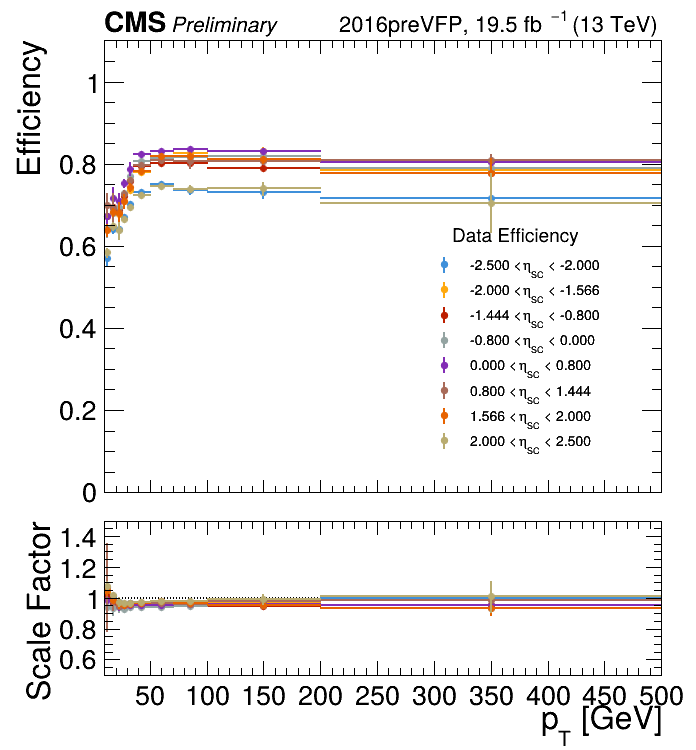
\includegraphics[width=0.45\textwidth]{Figures/analysis/EleID_eff_2016preVFP.png}}
  \hfill
  \subfloat[2016 postVFP]{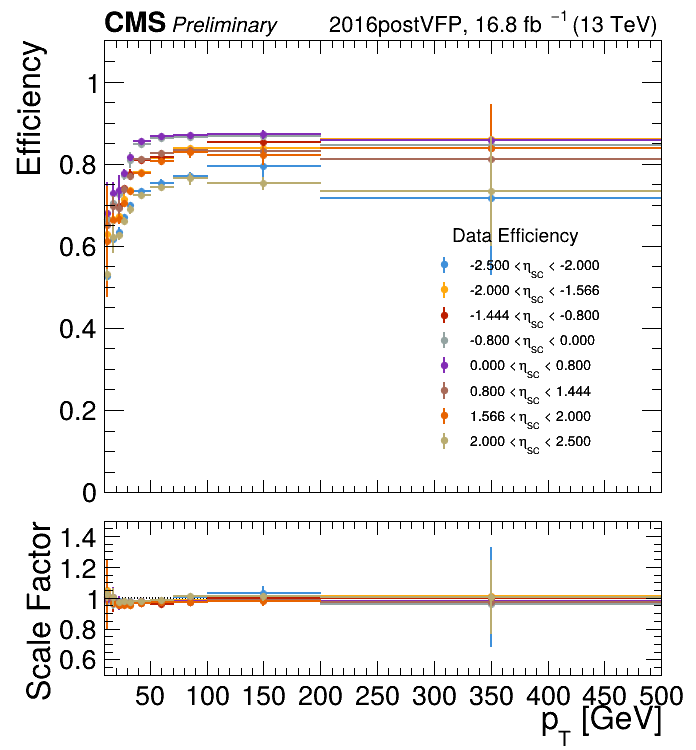
\includegraphics[width=0.45\textwidth]{Figures/analysis/EleID_eff_2016postVFP.png}} \\
  \subfloat[2017]{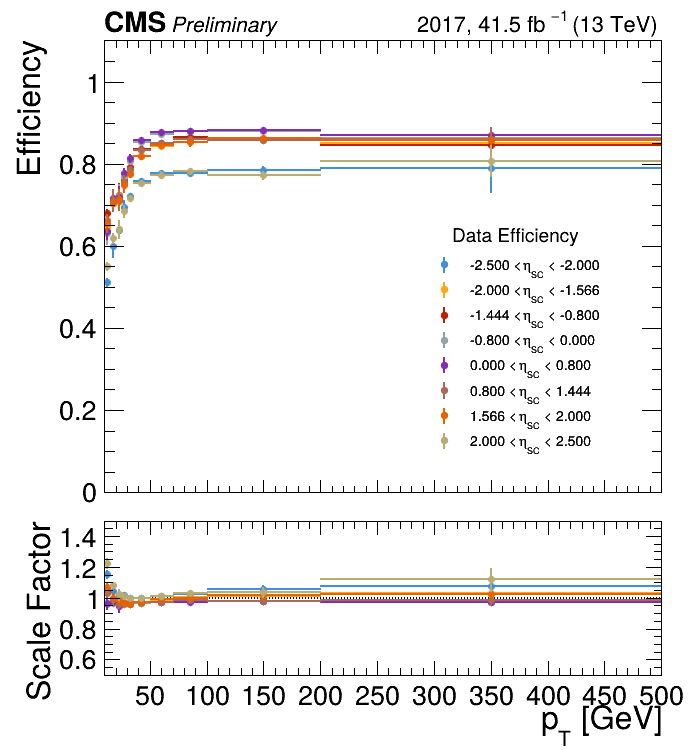
\includegraphics[width=0.45\textwidth]{Figures/analysis/EleID_eff_2017.png}}
  \hfill
  \subfloat[2018]{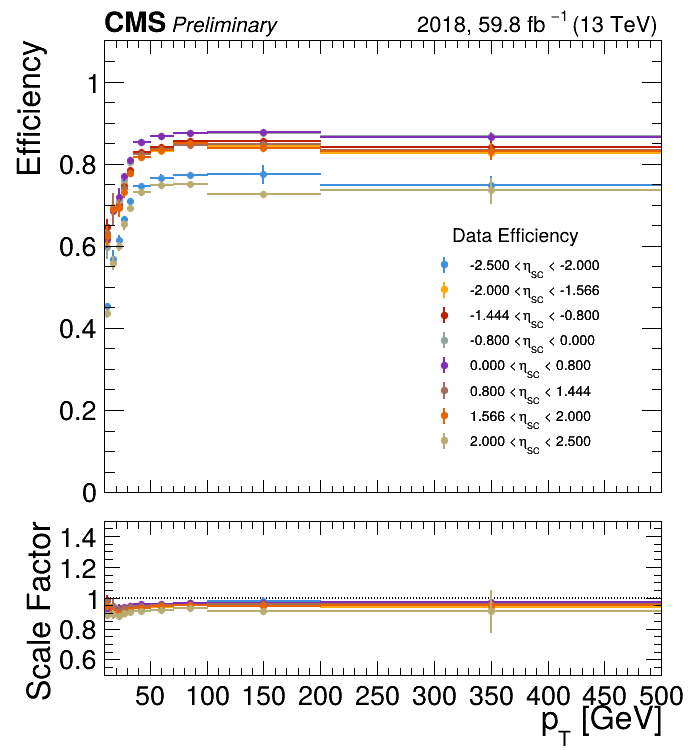
\includegraphics[width=0.45\textwidth]{Figures/analysis/EleID_eff_2018.png}}
  \caption{Electron identification efficiency as a function of $\pT$ in bins of $\eta_\text{SC}$ for the Run~2 data-taking periods. The upper panels show the data efficiency and the lower panels show the data-to-simulation scale factor.}
  \label{fig:eleid_eff_run2}
\end{figure}

\begin{figure}[htbp]
  \centering
  \subfloat[2022]{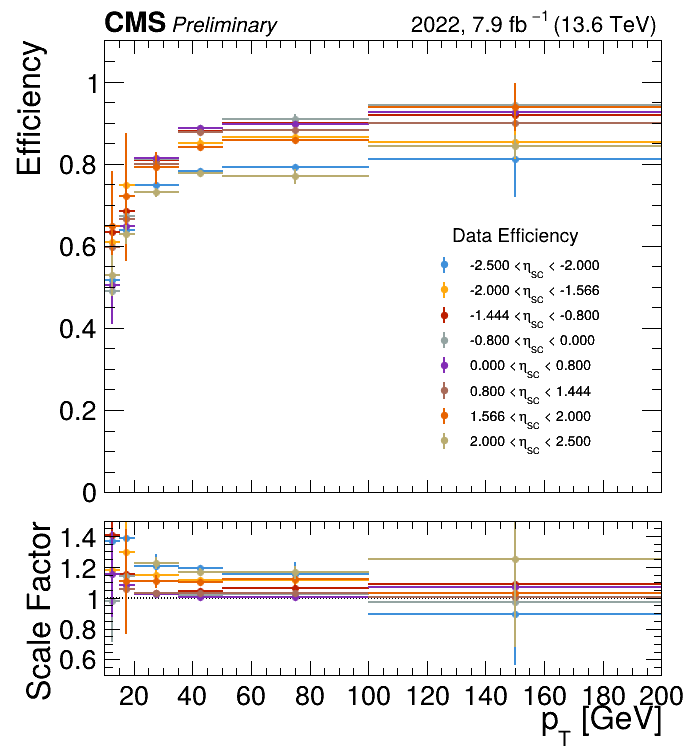
\includegraphics[width=0.45\textwidth]{Figures/analysis/EleID_eff_2022.png}}
  \hfill
  \subfloat[2022EE]{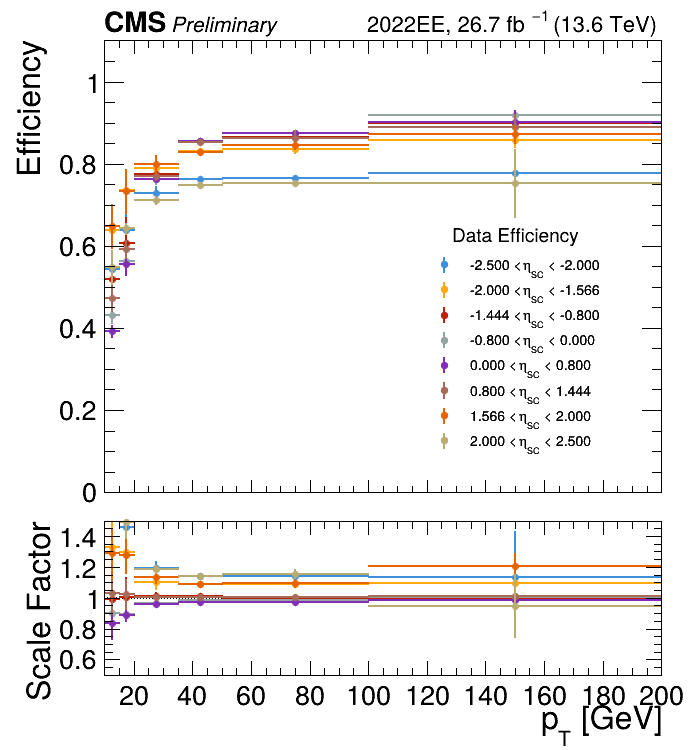
\includegraphics[width=0.45\textwidth]{Figures/analysis/EleID_eff_2022EE.png}} \\
  \subfloat[2023]{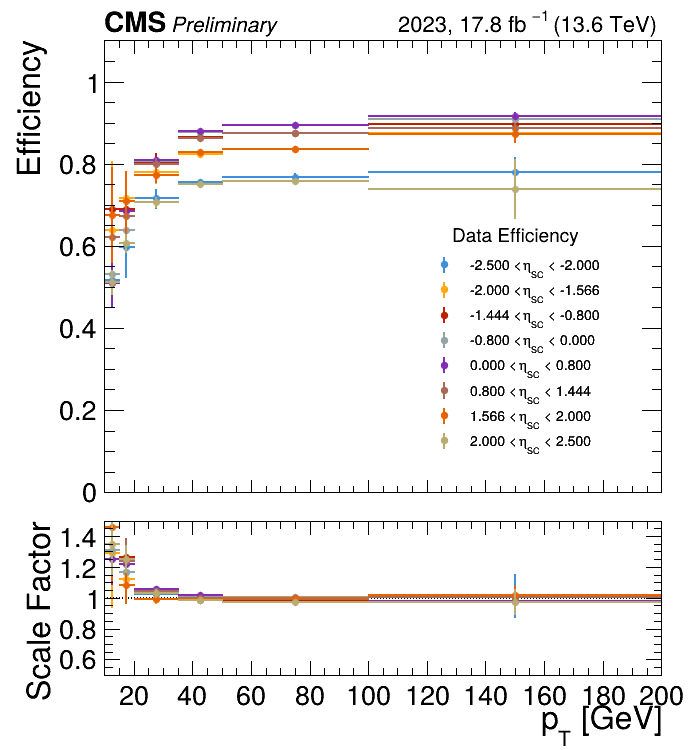
\includegraphics[width=0.45\textwidth]{Figures/analysis/EleID_eff_2023.png}}
  \hfill
  \subfloat[2023BPix]{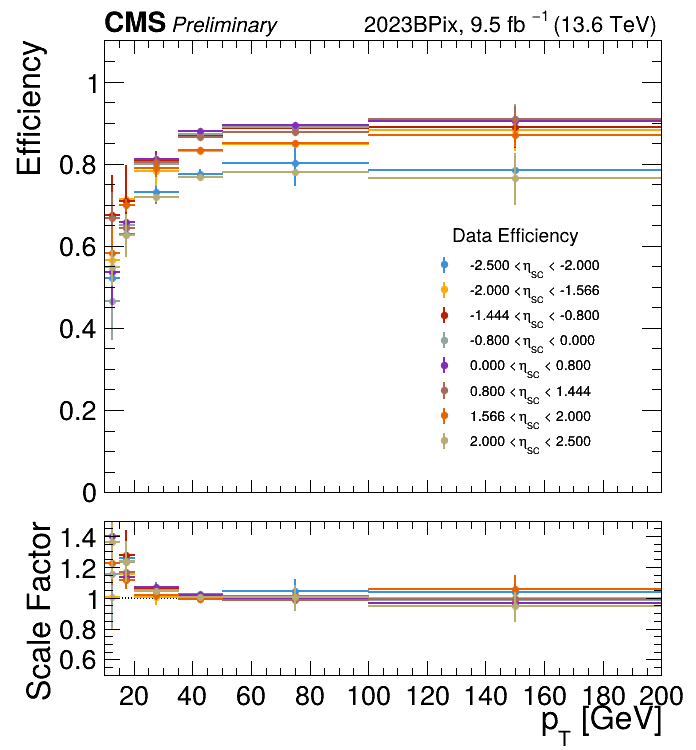
\includegraphics[width=0.45\textwidth]{Figures/analysis/EleID_eff_2023BPix.png}}
  \caption{Electron identification efficiency as a function of $\pT$ in bins of $\eta_\text{SC}$ for the Run~3 data-taking periods. The upper panels show the data efficiency and the lower panels show the data-to-simulation scale factor.}
  \label{fig:eleid_eff_run3}
\end{figure}

\begin{figure}[htbp]
  \centering
  \subfloat[2016 preVFP]{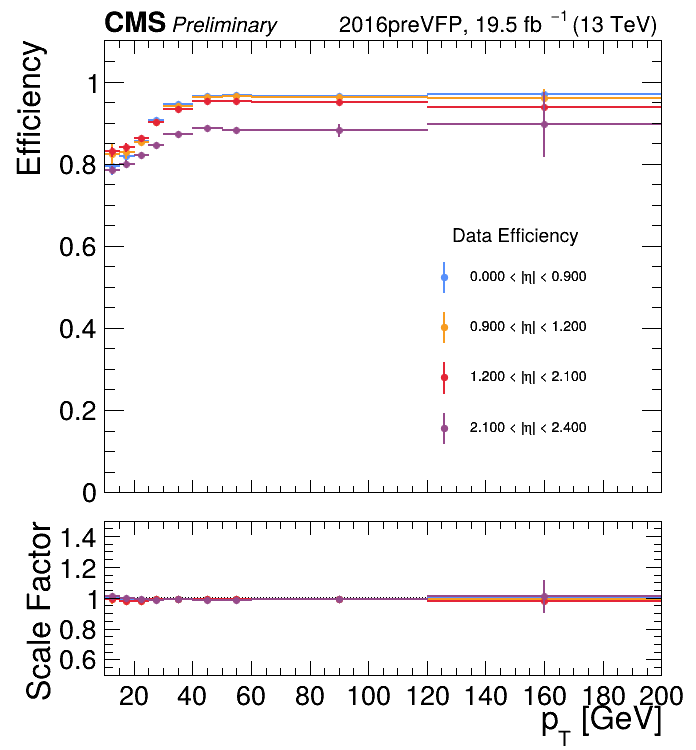
\includegraphics[width=0.45\textwidth]{Figures/analysis/MuID_eff_2016preVFP.png}}
  \hfill
  \subfloat[2016 postVFP]{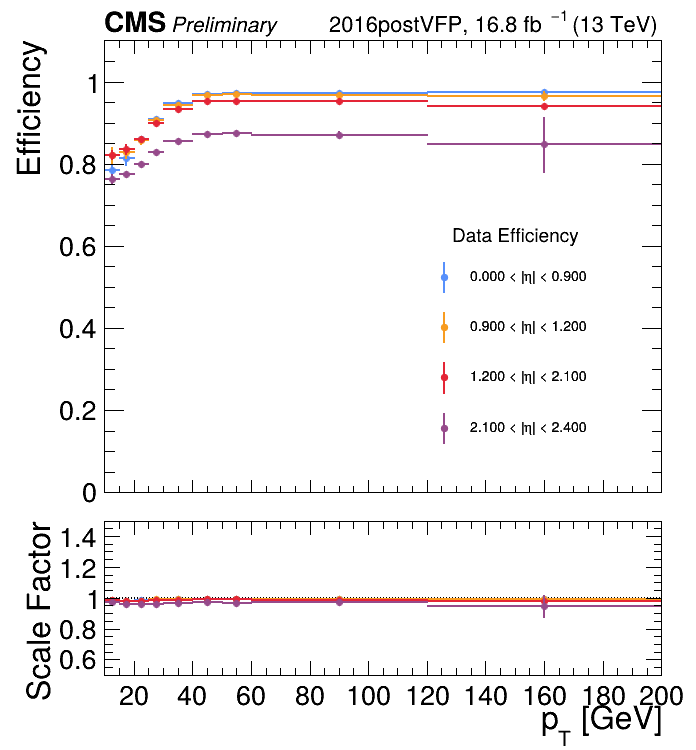
\includegraphics[width=0.45\textwidth]{Figures/analysis/MuID_eff_2016postVFP.png}} \\
  \subfloat[2017]{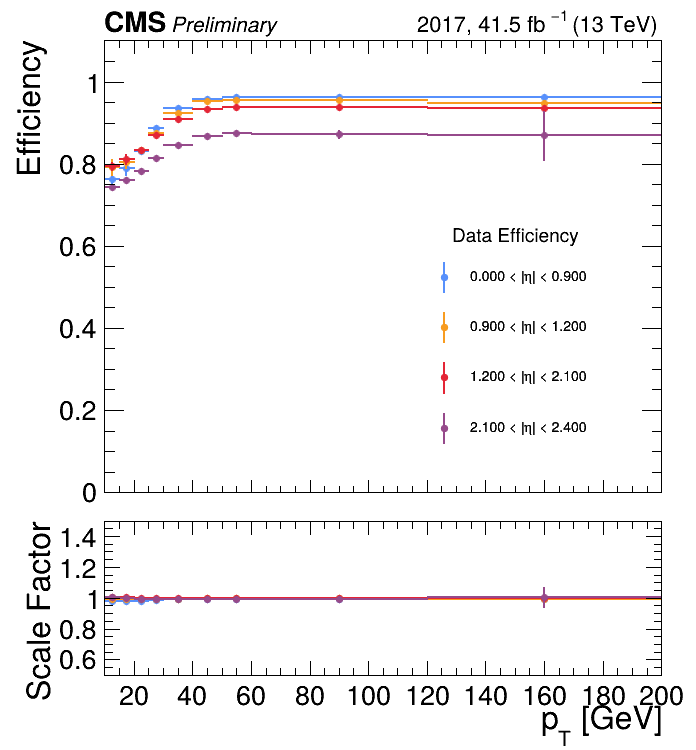
\includegraphics[width=0.45\textwidth]{Figures/analysis/MuID_eff_2017.png}}
  \hfill
  \subfloat[2018]{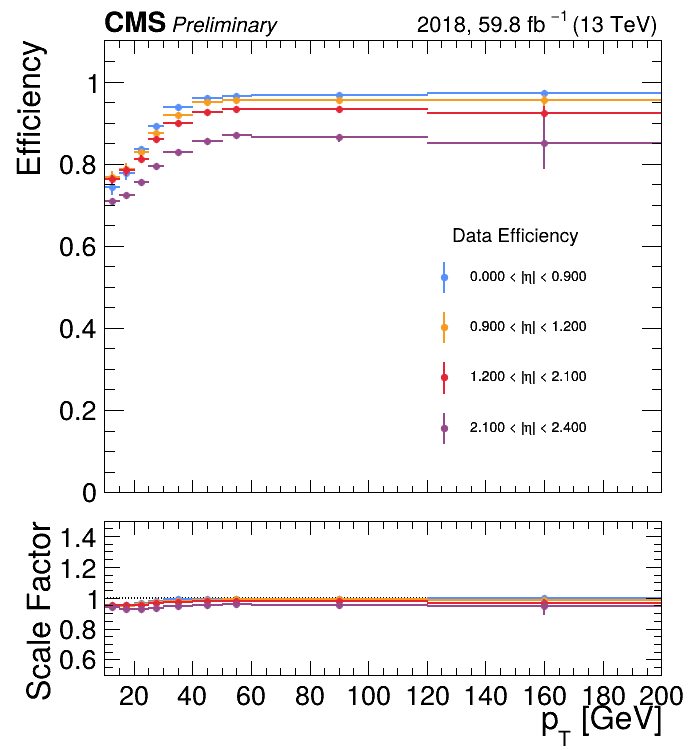
\includegraphics[width=0.45\textwidth]{Figures/analysis/MuID_eff_2018.png}}
  \caption{Muon identification efficiency as a function of $\pT$ in bins of $\eta$ for the Run~2 data-taking periods. The upper panels show the data efficiency and the lower panels show the data-to-simulation scale factor.}
  \label{fig:muid_eff_run2}
\end{figure}

\begin{figure}[htbp]
  \centering
  \subfloat[2022]{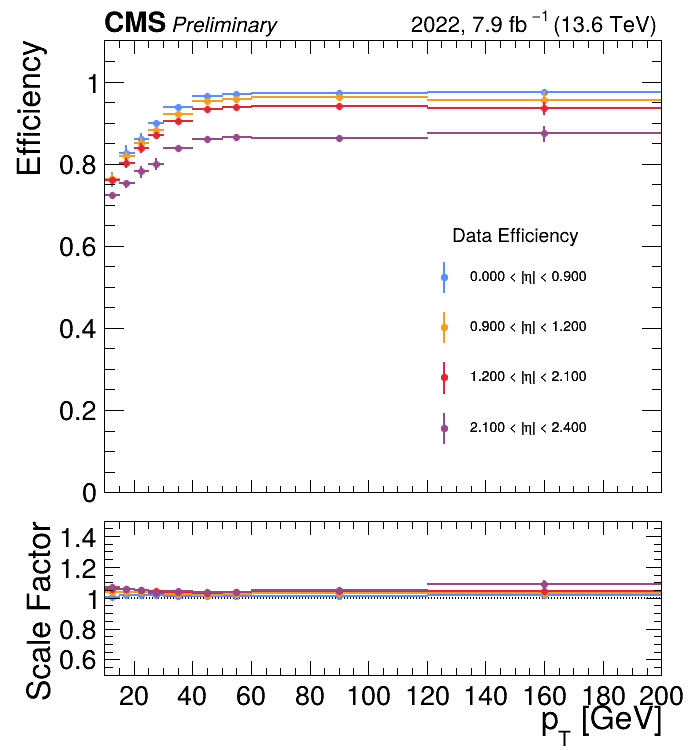
\includegraphics[width=0.45\textwidth]{Figures/analysis/MuID_eff_2022.png}}
  \hfill
  \subfloat[2022EE]{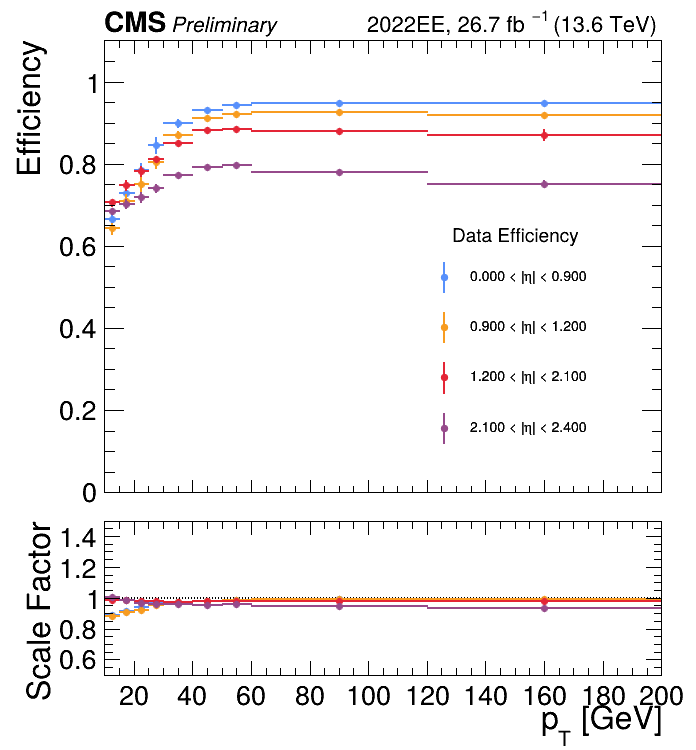
\includegraphics[width=0.45\textwidth]{Figures/analysis/MuID_eff_2022EE.png}} \\
  \subfloat[2023]{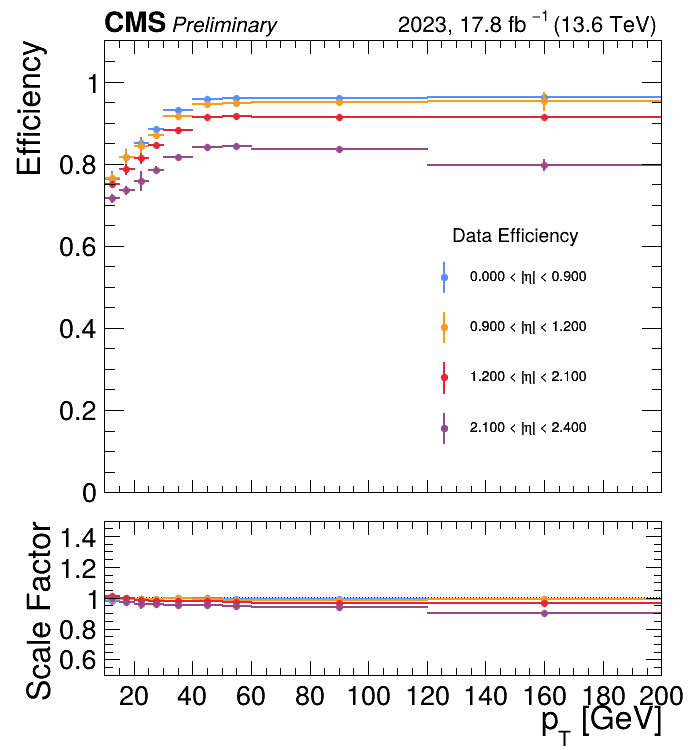
\includegraphics[width=0.45\textwidth]{Figures/analysis/MuID_eff_2023.png}}
  \hfill
  \subfloat[2023BPix]{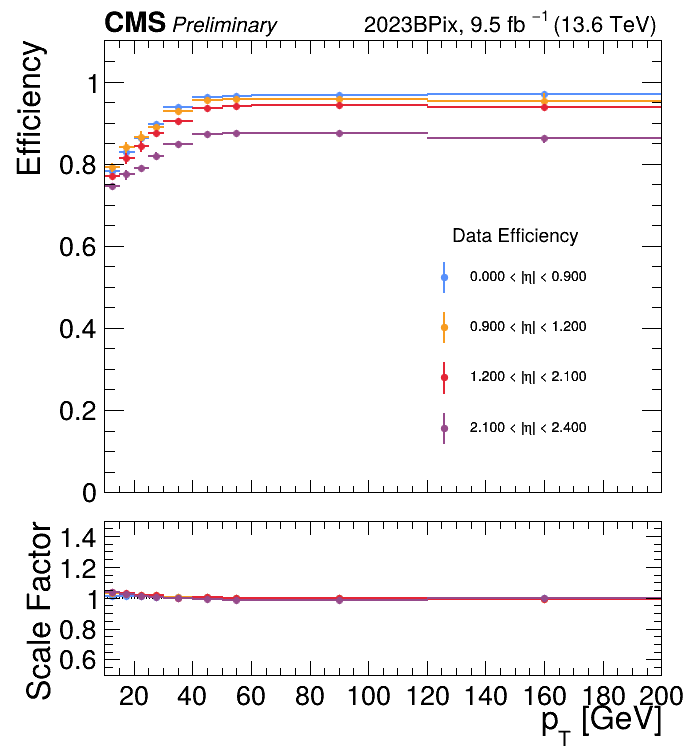
\includegraphics[width=0.45\textwidth]{Figures/analysis/MuID_eff_2023BPix.png}}
  \caption{Muon identification efficiency as a function of $\pT$ in bins of $\eta$ for the Run~3 data-taking periods. The upper panels show the data efficiency and the lower panels show the data-to-simulation scale factor.}
  \label{fig:muid_eff_run3}
\end{figure}

\subsubsection*{Trigger efficiency}

The dilepton trigger efficiency is factorized into per-lepton leg efficiencies and a pairwise filter efficiency:
\begin{equation}
\label{eq:trig_dilep}
\varepsilon(\ell_1, \ell_2) = \varepsilon_\text{leg1}(\ell_1) \times \varepsilon_\text{leg2}(\ell_2) \times \varepsilon_\text{pair}\,,
\end{equation}
where $\varepsilon_\text{leg1}$ and $\varepsilon_\text{leg2}$ denote the efficiencies for the leading and subleading trigger legs, measured as functions of $\pT$ and $\eta$ using the tag-and-probe method, and $\varepsilon_\text{pair}$ accounts for the pairwise vertex-compatibility filter applied in several trigger paths. The pairwise filter efficiency is measured using a reference trigger method and is found to be consistent with unity at the sub-percent level for all eras.

For three-lepton events, the trigger efficiency accounts for the combinatorial possibility that any qualifying lepton pair may fire the trigger. In the $\Pgm\Pgm\Pgm$ channel using dimuon triggers, the efficiency for an event with three muons ordered by $\pT$ ($\mu_1, \mu_2, \mu_3$) is:
\begin{align}
\label{eq:trig_3mu}
\varepsilon(\mu_1, \mu_2, \mu_3) &= \varepsilon_\text{leg1}(\mu_1) \left[ \varepsilon_\text{leg2}(\mu_2)\,\varepsilon_\text{pair} + \left(1 - \varepsilon_\text{leg2}(\mu_2)\right) \varepsilon_\text{leg2}(\mu_3)\,\varepsilon_\text{pair} \right] \nonumber \\
&\quad + \left(1 - \varepsilon_\text{leg1}(\mu_1)\right) \varepsilon_\text{leg1}(\mu_2)\,\varepsilon_\text{leg2}(\mu_3)\,\varepsilon_\text{pair}\,.
\end{align}
In the $\Pe\Pgm\Pgm$ channel using electron-muon cross-triggers, the efficiency for an event with one electron and two muons is:
\begin{equation}
\label{eq:trig_emu}
\varepsilon(e, \mu_1, \mu_2) = \varepsilon_e(e) \left[ \varepsilon_\mu(\mu_1)\,\varepsilon_\text{pair} + \left(1 - \varepsilon_\mu(\mu_1)\right) \varepsilon_\mu(\mu_2)\,\varepsilon_\text{pair} \right] .
\end{equation}
The trigger scale factor for each event is computed as the ratio of the data and MC efficiencies:
\begin{equation}
\text{SF}_\text{trig} = \frac{\varepsilon_\text{data}}{\varepsilon_\text{MC}}\,.
\end{equation}

The measured per-leg trigger efficiencies for the dimuon triggers are shown in Figs.~\ref{fig:trig_dblmu17_run2}--\ref{fig:trig_dblmu8_run3} for the leading ($\pT > 17\GeV$) and subleading ($\pT > 8\GeV$) muon legs. For the electron-muon cross-triggers, two paths are used: \texttt{Mu23\_El12} (muon $\pT > 23\GeV$, electron $\pT > 12\GeV$) and \texttt{Mu8\_El23} (muon $\pT > 8\GeV$, electron $\pT > 23\GeV$). The per-leg efficiencies for all four legs are shown in Figs.~\ref{fig:trig_mu23el12_mu_run2}--\ref{fig:trig_mu8el23_el_run3}.

\begin{figure}[htbp]
  \centering
  \subfloat[2016 preVFP]{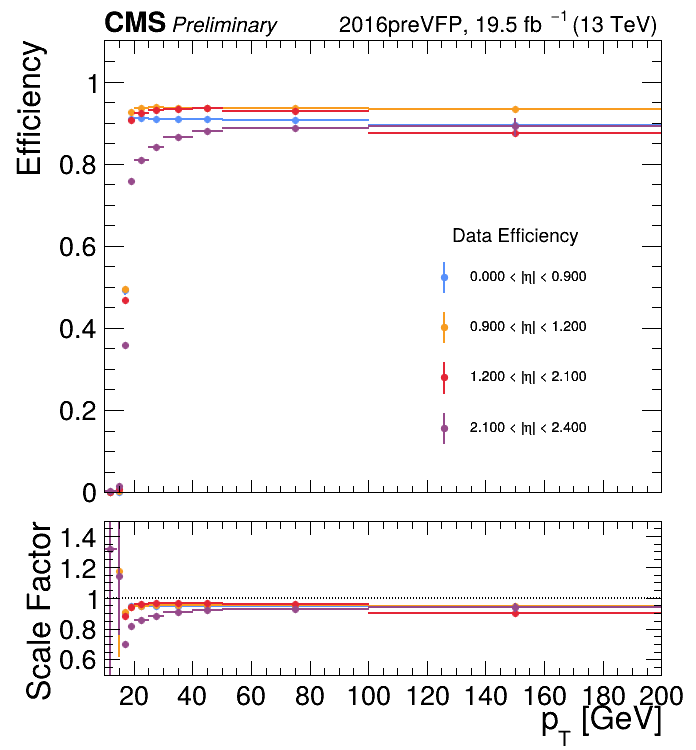
\includegraphics[width=0.45\textwidth]{Figures/analysis/DblMu_MU17Leg_eff_2016preVFP.png}}
  \hfill
  \subfloat[2016 postVFP]{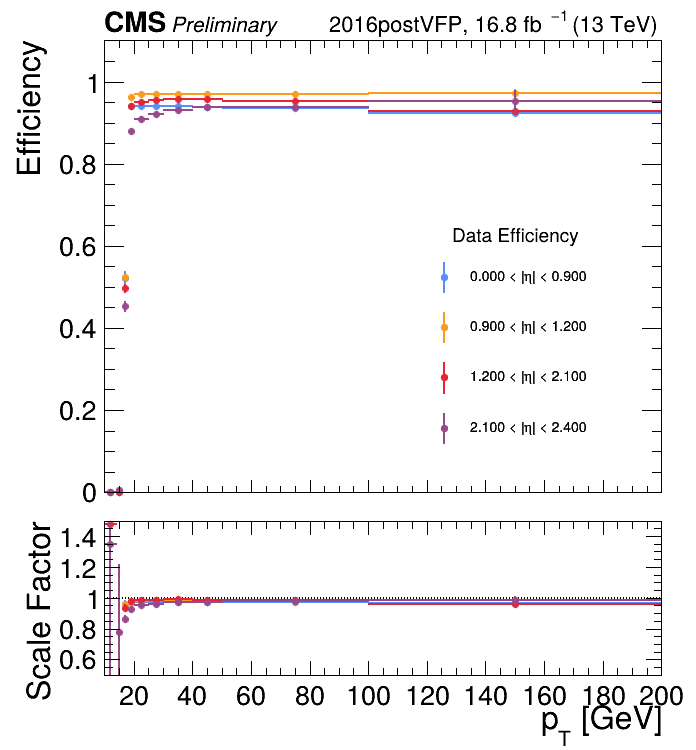
\includegraphics[width=0.45\textwidth]{Figures/analysis/DblMu_MU17Leg_eff_2016postVFP.png}} \\
  \subfloat[2017]{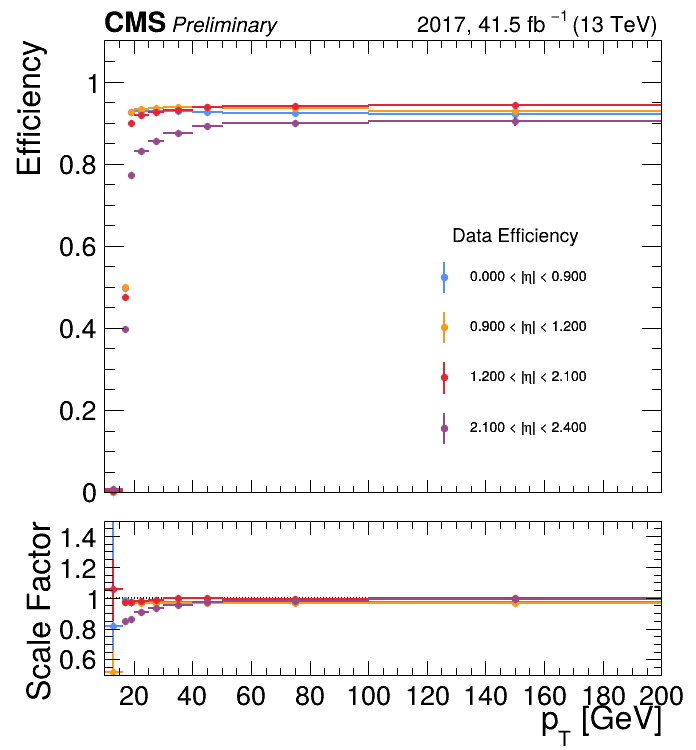
\includegraphics[width=0.45\textwidth]{Figures/analysis/DblMu_MU17Leg_eff_2017.png}}
  \hfill
  \subfloat[2018]{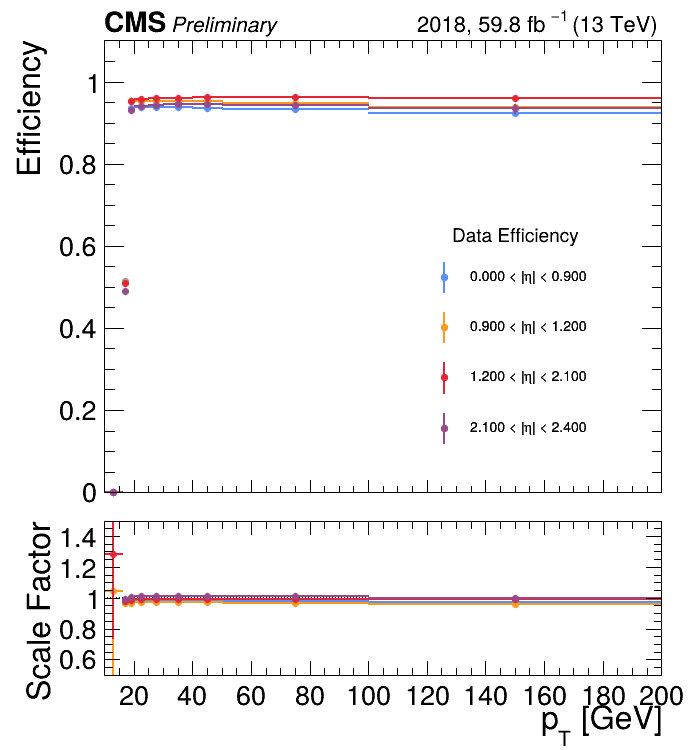
\includegraphics[width=0.45\textwidth]{Figures/analysis/DblMu_MU17Leg_eff_2018.png}}
  \caption{Dimuon trigger leading leg ($\pT > 17\GeV$) efficiency as a function of muon $\pT$ in bins of $\eta$ for the Run~2 data-taking periods.}
  \label{fig:trig_dblmu17_run2}
\end{figure}

\begin{figure}[htbp]
  \centering
  \subfloat[2022]{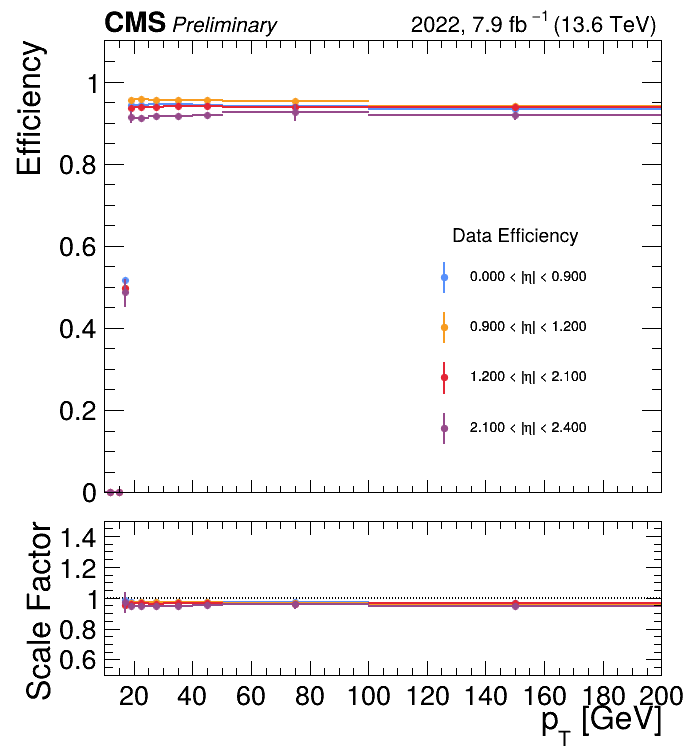
\includegraphics[width=0.45\textwidth]{Figures/analysis/DblMu_MU17Leg_eff_2022.png}}
  \hfill
  \subfloat[2022EE]{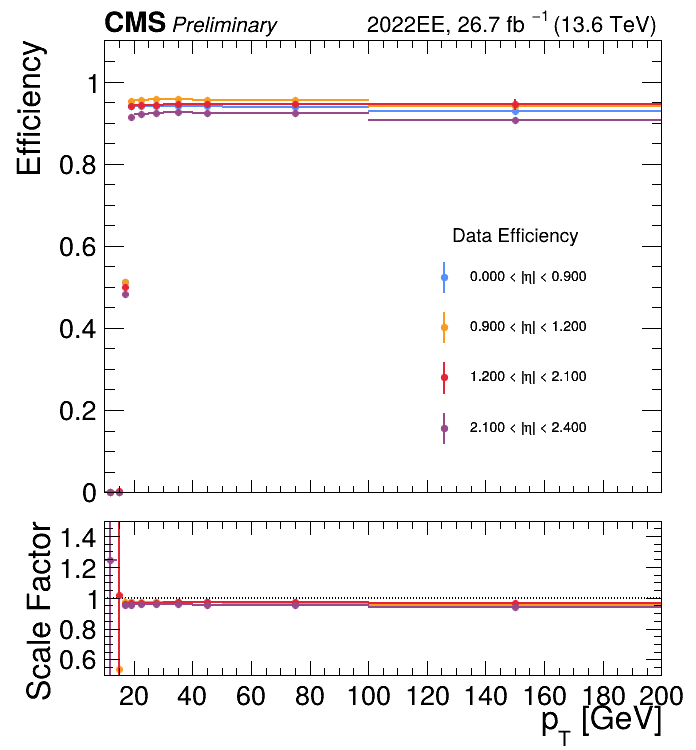
\includegraphics[width=0.45\textwidth]{Figures/analysis/DblMu_MU17Leg_eff_2022EE.png}} \\
  \subfloat[2023]{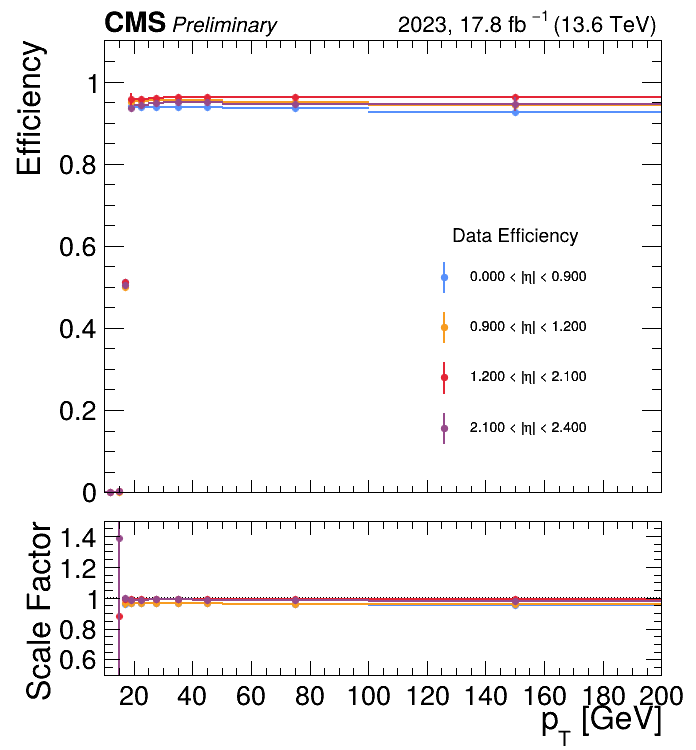
\includegraphics[width=0.45\textwidth]{Figures/analysis/DblMu_MU17Leg_eff_2023.png}}
  \hfill
  \subfloat[2023BPix]{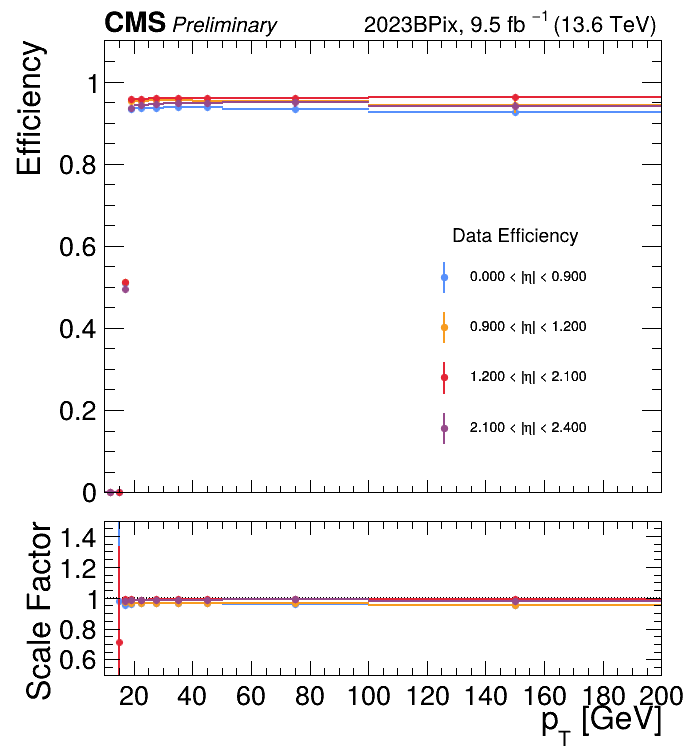
\includegraphics[width=0.45\textwidth]{Figures/analysis/DblMu_MU17Leg_eff_2023BPix.png}}
  \caption{Dimuon trigger leading leg ($\pT > 17\GeV$) efficiency as a function of muon $\pT$ in bins of $\eta$ for the Run~3 data-taking periods.}
  \label{fig:trig_dblmu17_run3}
\end{figure}

\begin{figure}[htbp]
  \centering
  \subfloat[2016 preVFP]{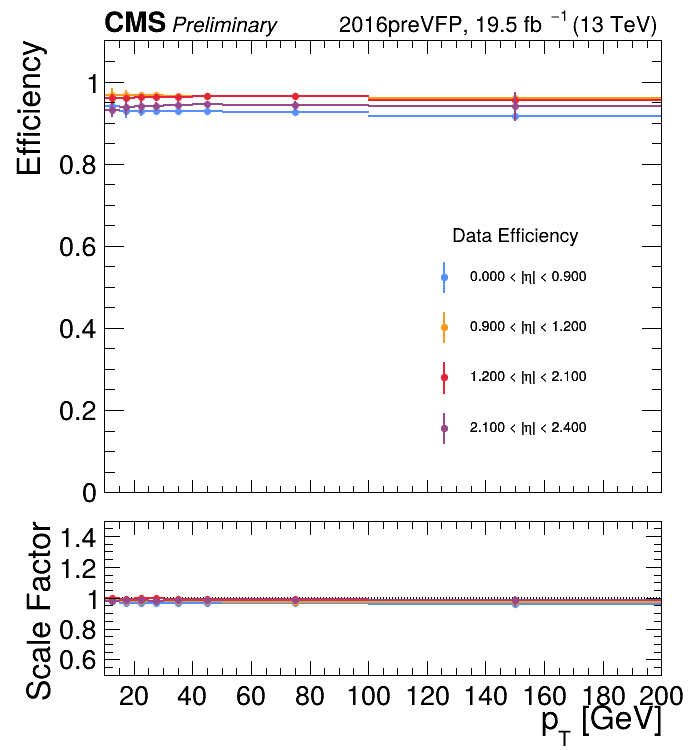
\includegraphics[width=0.45\textwidth]{Figures/analysis/DblMu_MU8Leg_eff_2016preVFP.png}}
  \hfill
  \subfloat[2016 postVFP]{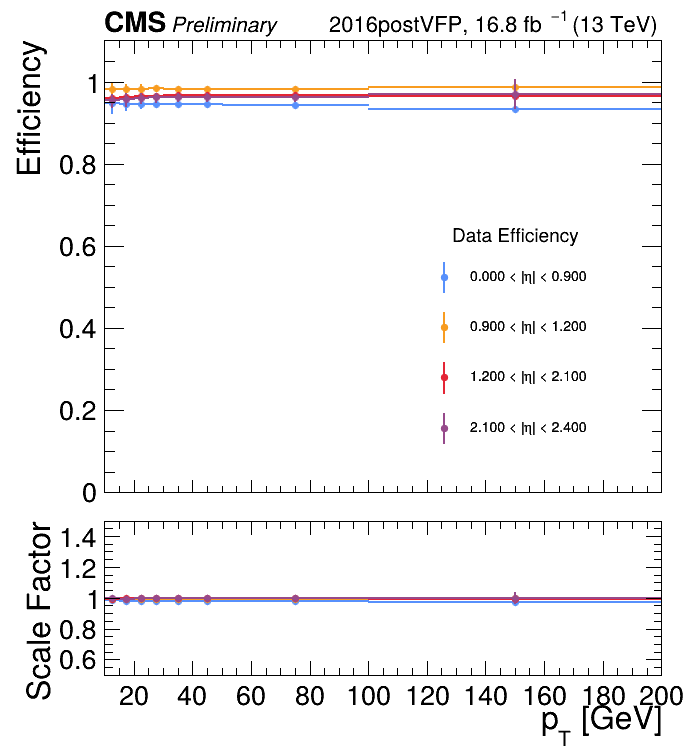
\includegraphics[width=0.45\textwidth]{Figures/analysis/DblMu_MU8Leg_eff_2016postVFP.png}} \\
  \subfloat[2017]{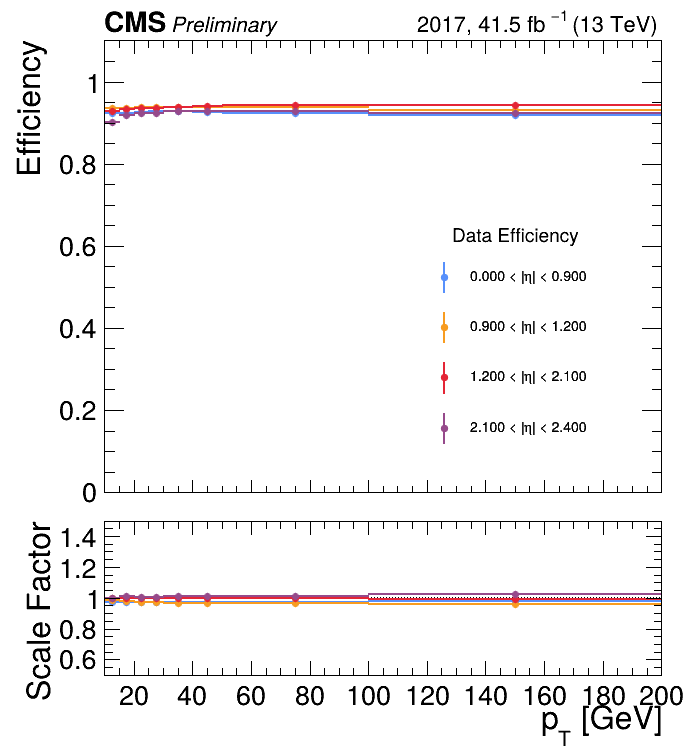
\includegraphics[width=0.45\textwidth]{Figures/analysis/DblMu_MU8Leg_eff_2017.png}}
  \hfill
  \subfloat[2018]{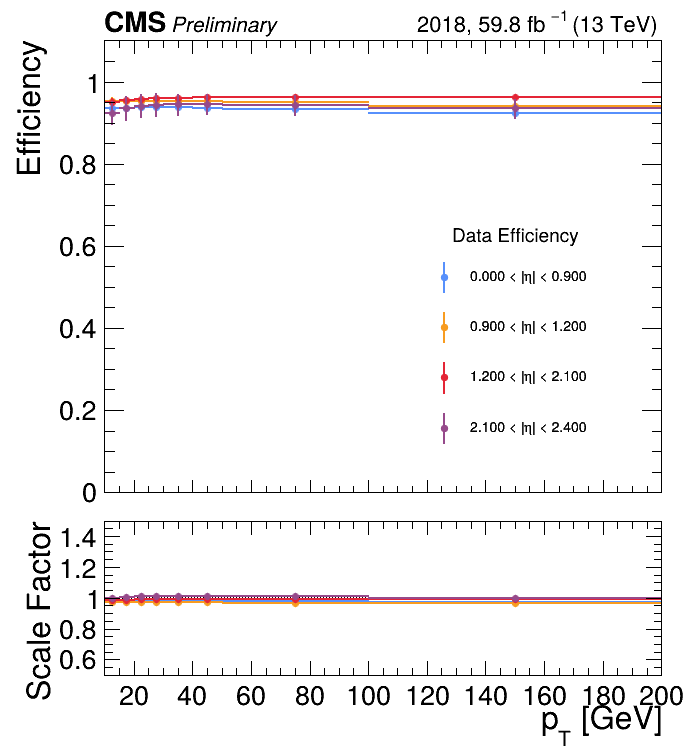
\includegraphics[width=0.45\textwidth]{Figures/analysis/DblMu_MU8Leg_eff_2018.png}}
  \caption{Dimuon trigger subleading leg ($\pT > 8\GeV$) efficiency as a function of muon $\pT$ in bins of $\eta$ for the Run~2 data-taking periods.}
  \label{fig:trig_dblmu8_run2}
\end{figure}

\begin{figure}[htbp]
  \centering
  \subfloat[2022]{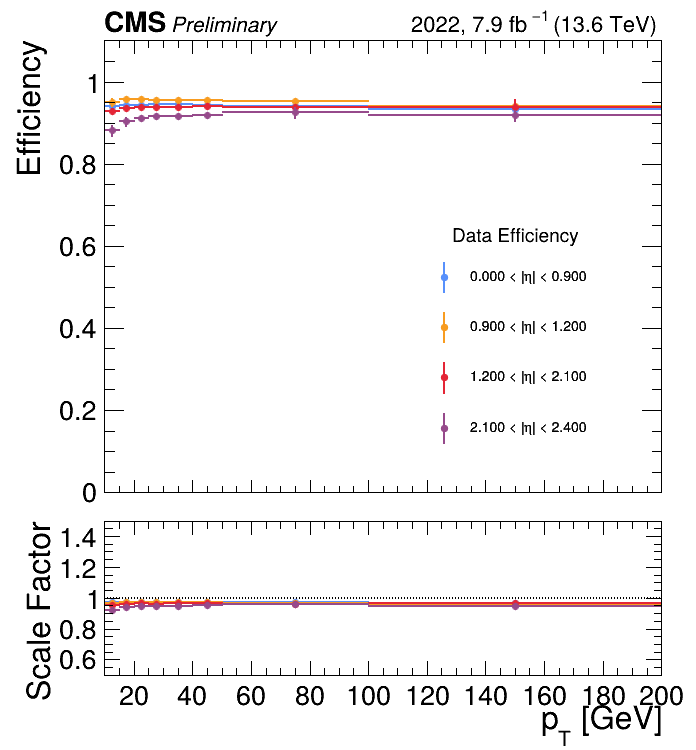
\includegraphics[width=0.45\textwidth]{Figures/analysis/DblMu_MU8Leg_eff_2022.png}}
  \hfill
  \subfloat[2022EE]{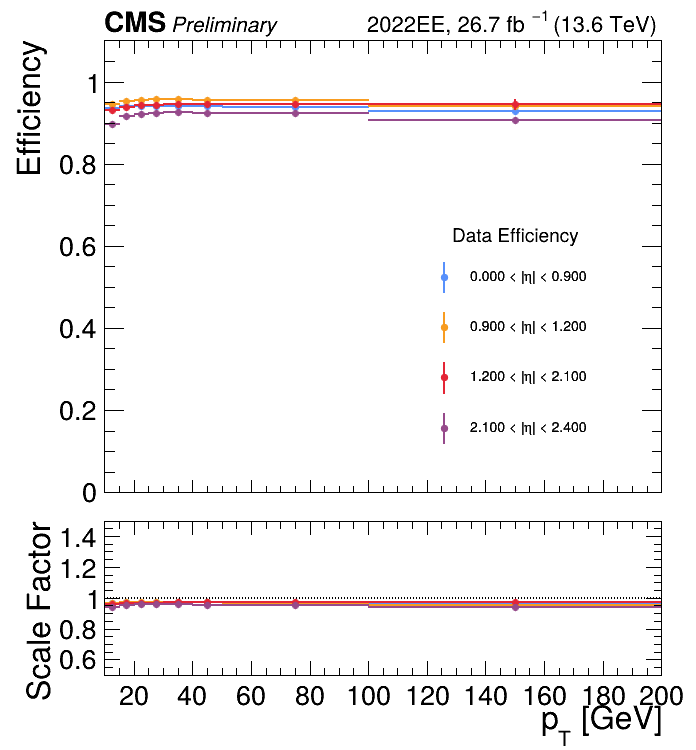
\includegraphics[width=0.45\textwidth]{Figures/analysis/DblMu_MU8Leg_eff_2022EE.png}} \\
  \subfloat[2023]{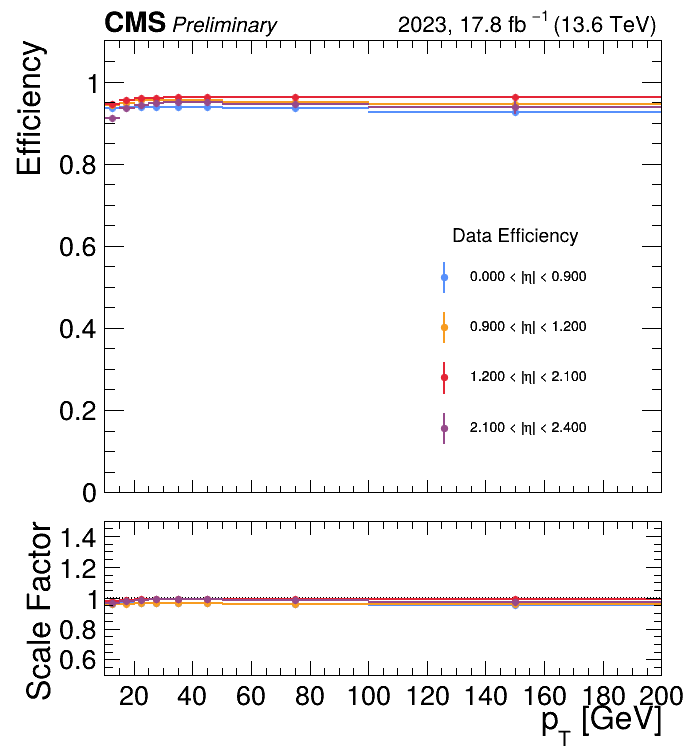
\includegraphics[width=0.45\textwidth]{Figures/analysis/DblMu_MU8Leg_eff_2023.png}}
  \hfill
  \subfloat[2023BPix]{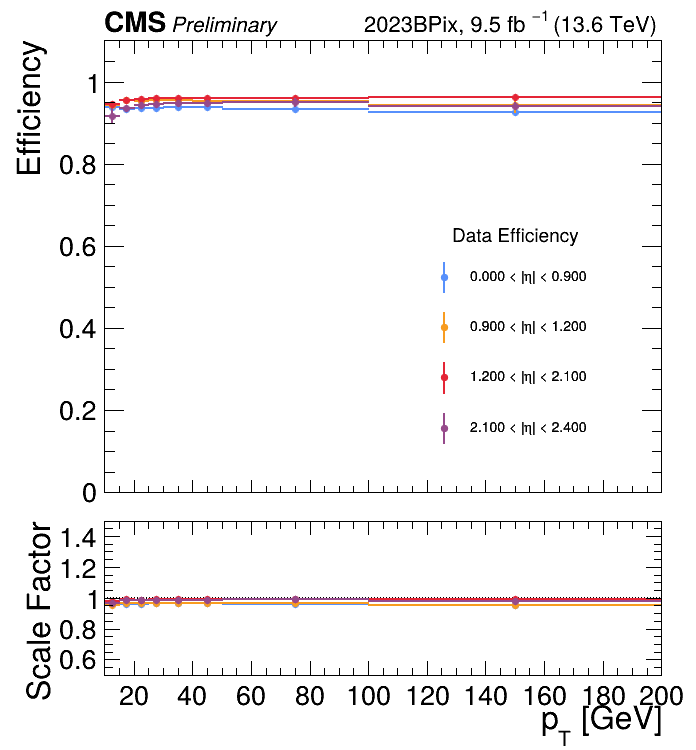
\includegraphics[width=0.45\textwidth]{Figures/analysis/DblMu_MU8Leg_eff_2023BPix.png}}
  \caption{Dimuon trigger subleading leg ($\pT > 8\GeV$) efficiency as a function of muon $\pT$ in bins of $\eta$ for the Run~3 data-taking periods.}
  \label{fig:trig_dblmu8_run3}
\end{figure}

\begin{figure}[htbp]
  \centering
  \subfloat[2016 preVFP]{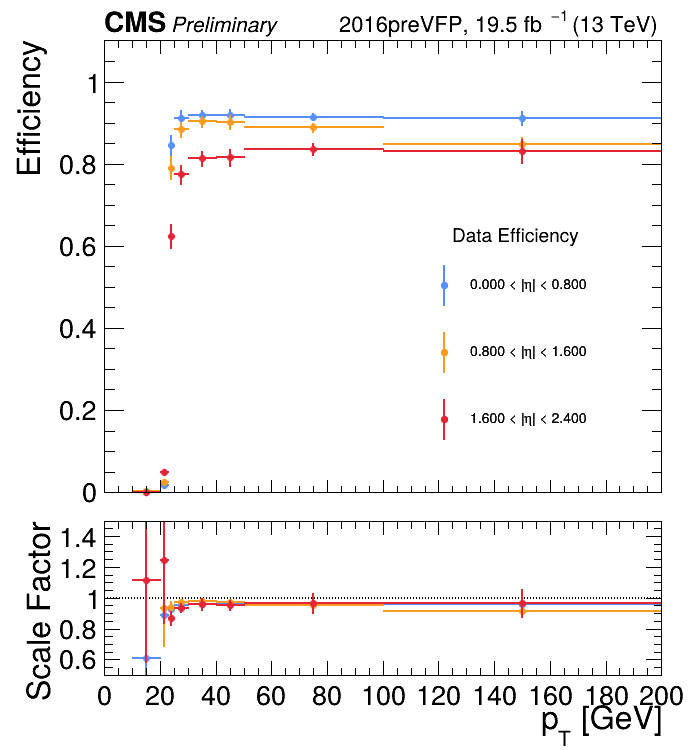
\includegraphics[width=0.45\textwidth]{Figures/analysis/Mu23El12_muon_eff_2016preVFP.png}}
  \hfill
  \subfloat[2016 postVFP]{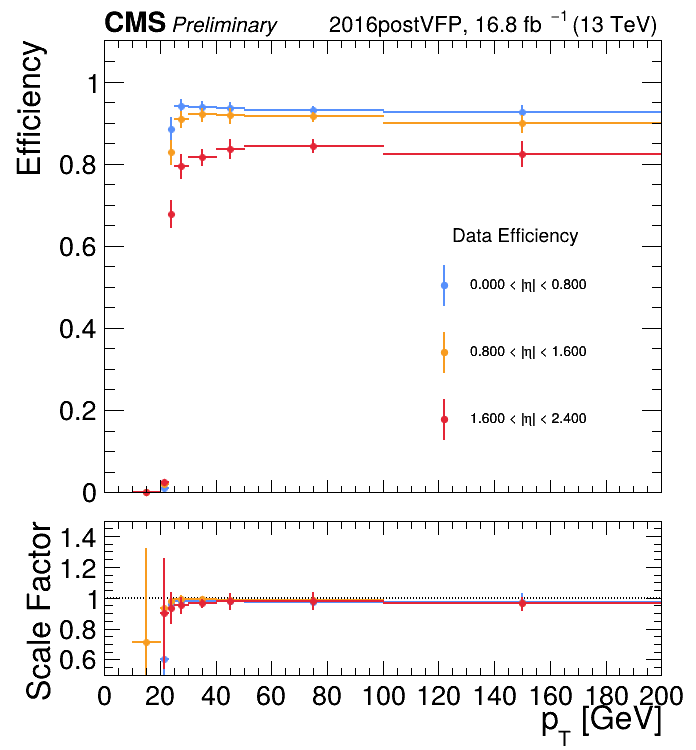
\includegraphics[width=0.45\textwidth]{Figures/analysis/Mu23El12_muon_eff_2016postVFP.png}} \\
  \subfloat[2017]{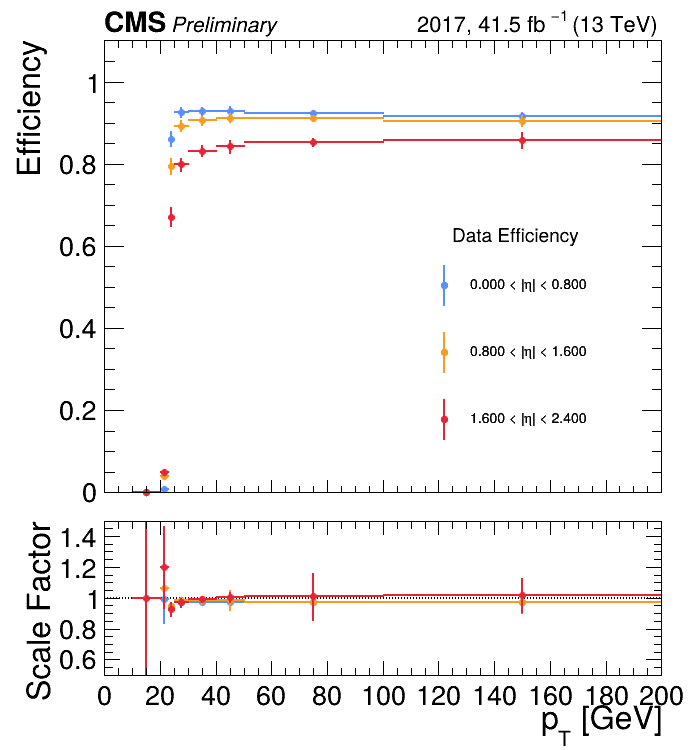
\includegraphics[width=0.45\textwidth]{Figures/analysis/Mu23El12_muon_eff_2017.png}}
  \hfill
  \subfloat[2018]{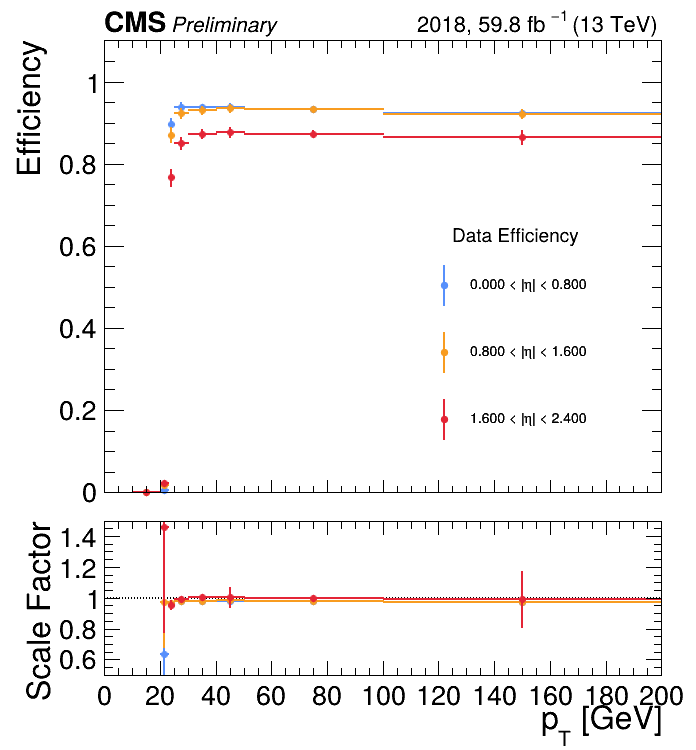
\includegraphics[width=0.45\textwidth]{Figures/analysis/Mu23El12_muon_eff_2018.png}}
  \caption{Muon leg ($\pT > 23\GeV$) efficiency for the \texttt{Mu23\_El12} cross-trigger as a function of muon $\pT$ in bins of $\eta$ for the Run~2 data-taking periods.}
  \label{fig:trig_mu23el12_mu_run2}
\end{figure}

\begin{figure}[htbp]
  \centering
  \subfloat[2022]{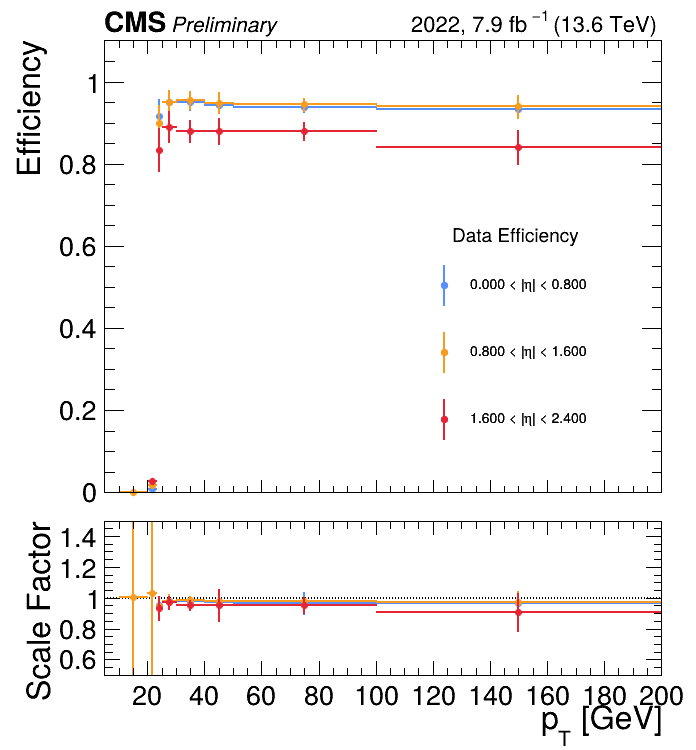
\includegraphics[width=0.45\textwidth]{Figures/analysis/Mu23El12_muon_eff_2022.png}}
  \hfill
  \subfloat[2022EE]{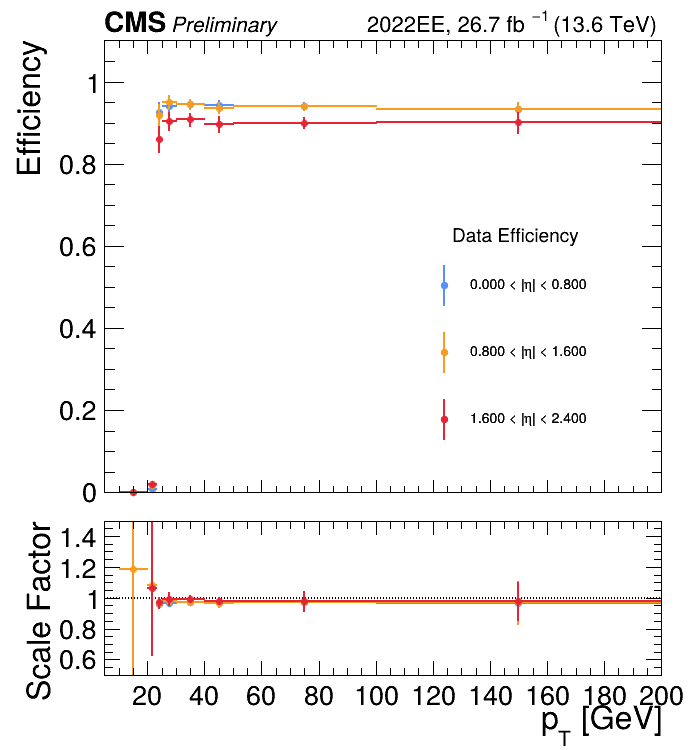
\includegraphics[width=0.45\textwidth]{Figures/analysis/Mu23El12_muon_eff_2022EE.png}} \\
  \subfloat[2023]{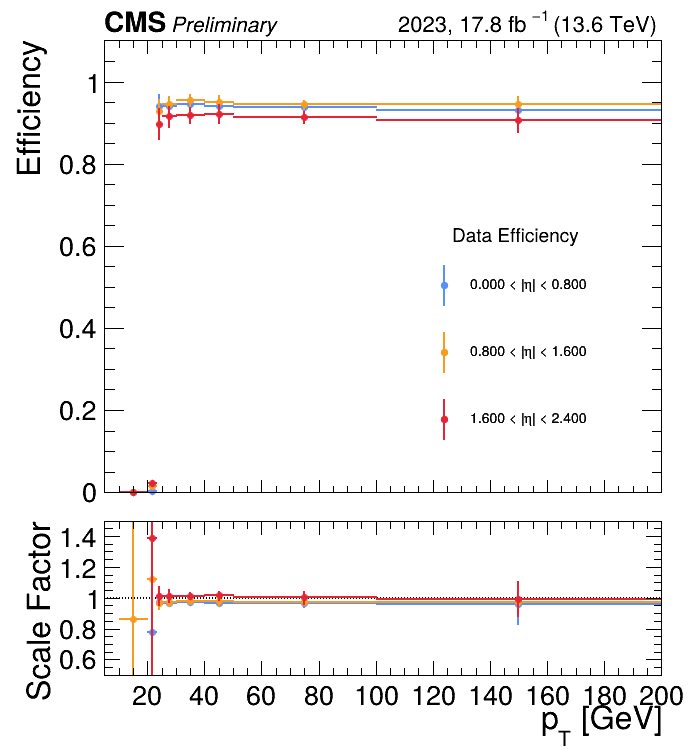
\includegraphics[width=0.45\textwidth]{Figures/analysis/Mu23El12_muon_eff_2023.png}}
  \hfill
  \subfloat[2023BPix]{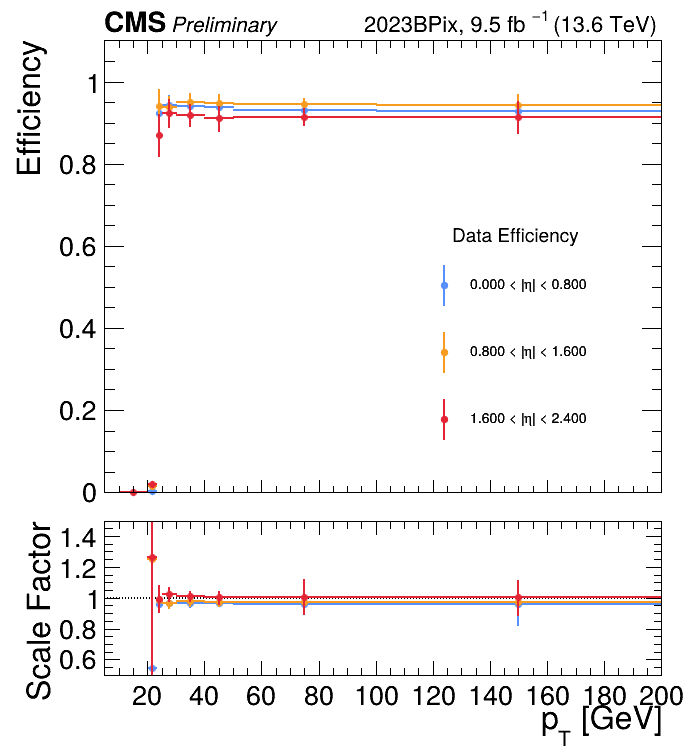
\includegraphics[width=0.45\textwidth]{Figures/analysis/Mu23El12_muon_eff_2023BPix.png}}
  \caption{Muon leg ($\pT > 23\GeV$) efficiency for the \texttt{Mu23\_El12} cross-trigger as a function of muon $\pT$ in bins of $\eta$ for the Run~3 data-taking periods.}
  \label{fig:trig_mu23el12_mu_run3}
\end{figure}

\begin{figure}[htbp]
  \centering
  \subfloat[2016 preVFP]{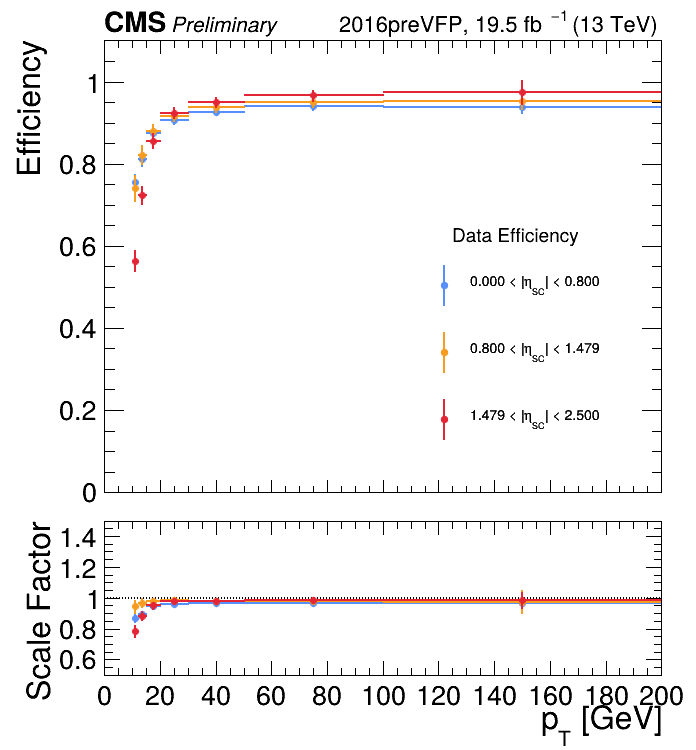
\includegraphics[width=0.45\textwidth]{Figures/analysis/Mu23El12_electron_eff_2016preVFP.png}}
  \hfill
  \subfloat[2016 postVFP]{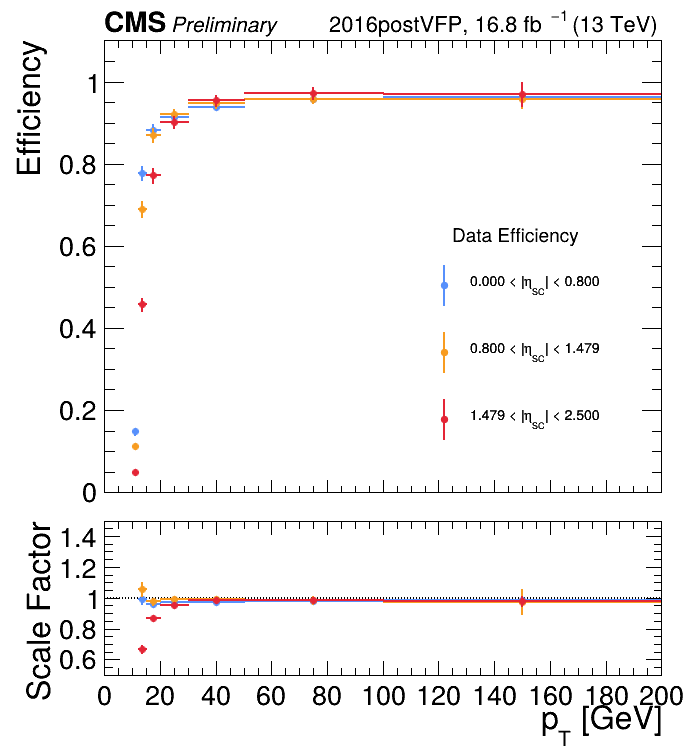
\includegraphics[width=0.45\textwidth]{Figures/analysis/Mu23El12_electron_eff_2016postVFP.png}} \\
  \subfloat[2017]{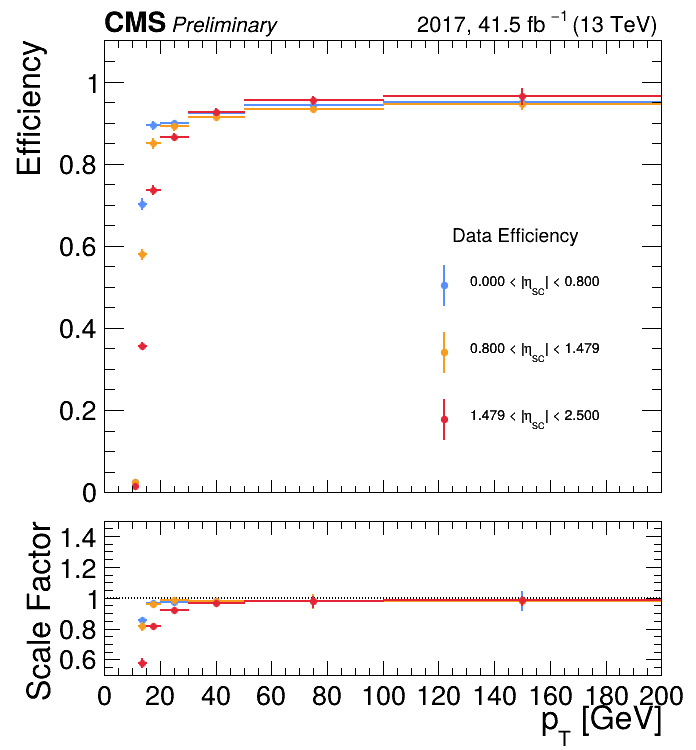
\includegraphics[width=0.45\textwidth]{Figures/analysis/Mu23El12_electron_eff_2017.png}}
  \hfill
  \subfloat[2018]{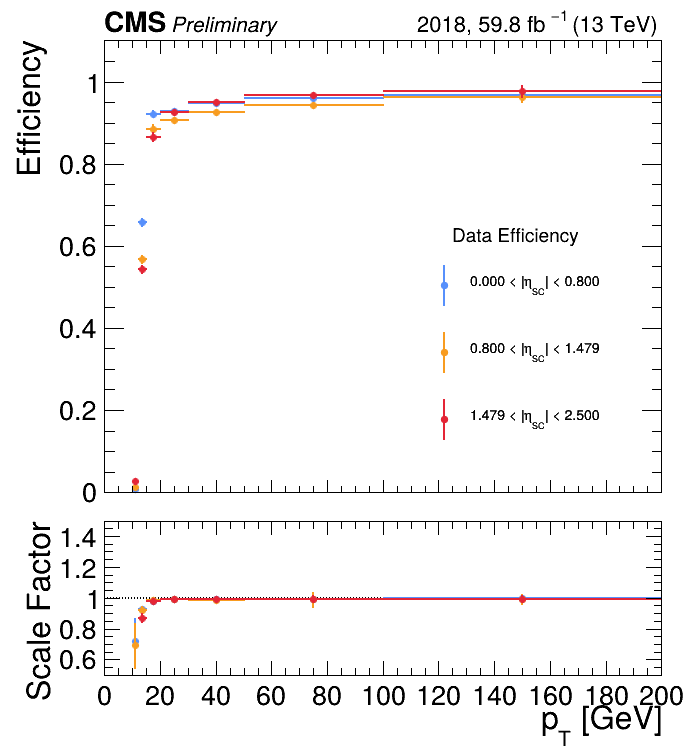
\includegraphics[width=0.45\textwidth]{Figures/analysis/Mu23El12_electron_eff_2018.png}}
  \caption{Electron leg ($\pT > 12\GeV$) efficiency for the \texttt{Mu23\_El12} cross-trigger as a function of electron $\pT$ in bins of $\eta_\text{SC}$ for the Run~2 data-taking periods.}
  \label{fig:trig_mu23el12_el_run2}
\end{figure}

\begin{figure}[htbp]
  \centering
  \subfloat[2022]{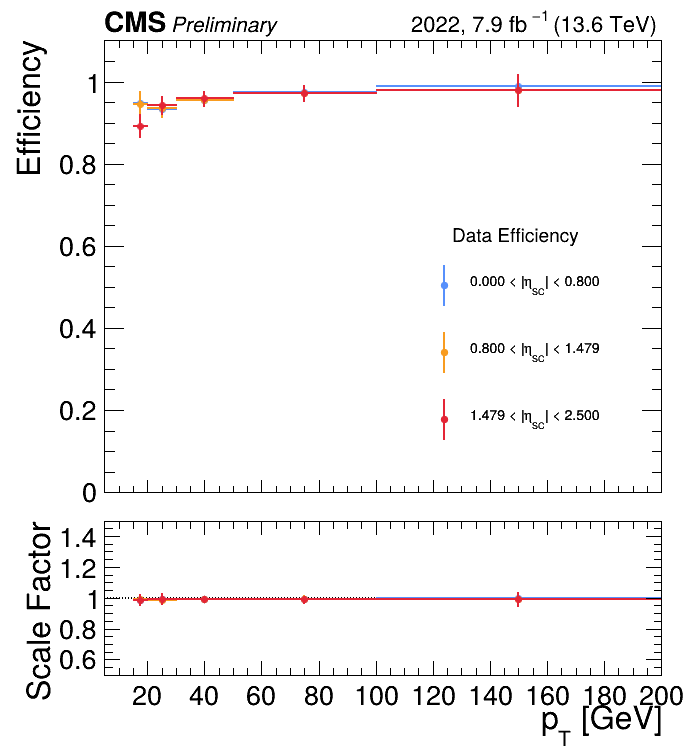
\includegraphics[width=0.45\textwidth]{Figures/analysis/Mu23El12_electron_eff_2022.png}}
  \hfill
  \subfloat[2022EE]{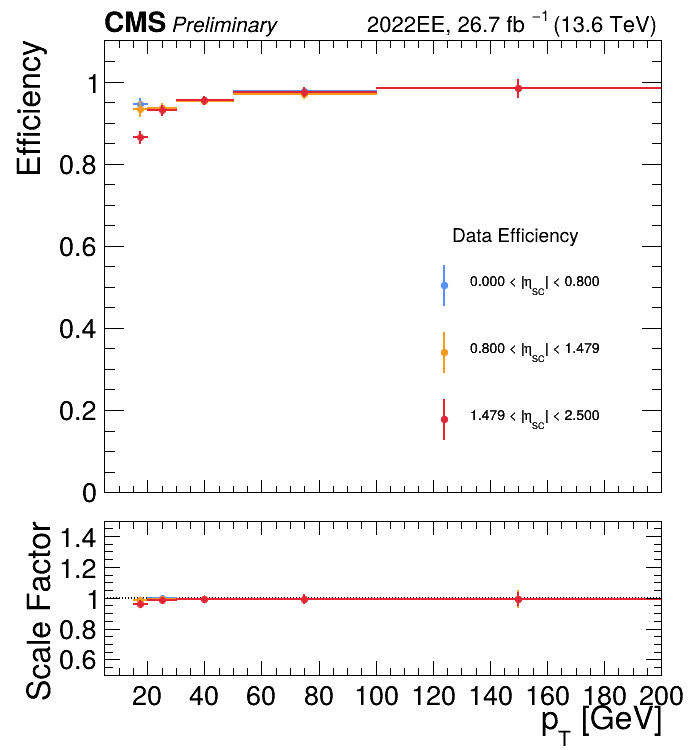
\includegraphics[width=0.45\textwidth]{Figures/analysis/Mu23El12_electron_eff_2022EE.png}} \\
  \subfloat[2023]{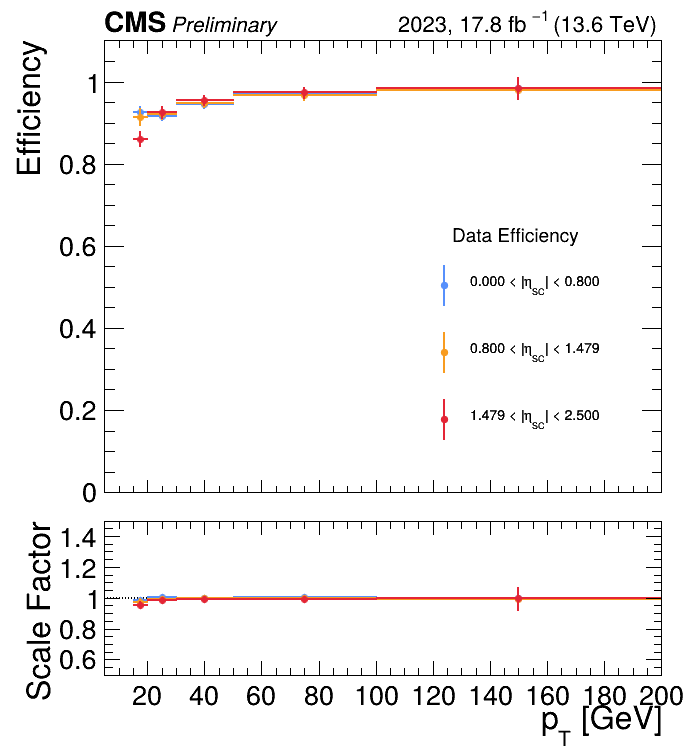
\includegraphics[width=0.45\textwidth]{Figures/analysis/Mu23El12_electron_eff_2023.png}}
  \hfill
  \subfloat[2023BPix]{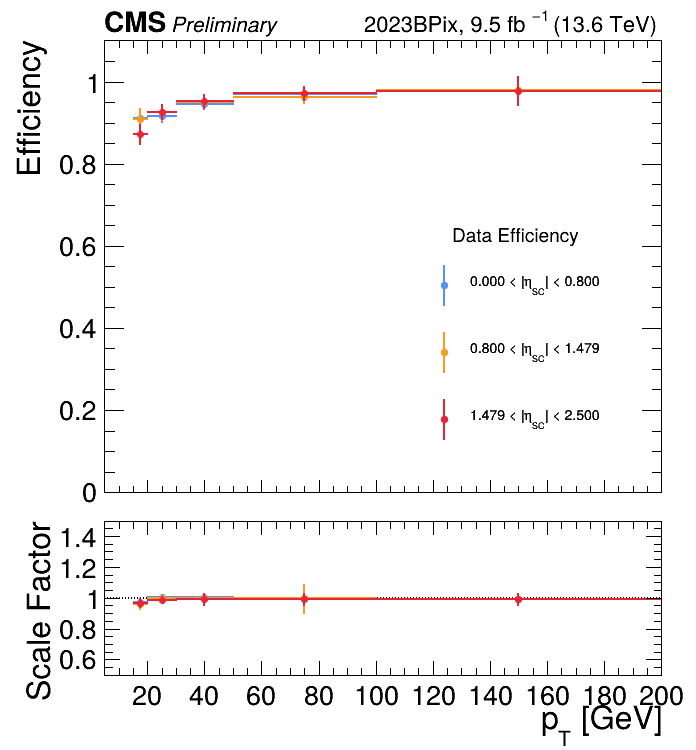
\includegraphics[width=0.45\textwidth]{Figures/analysis/Mu23El12_electron_eff_2023BPix.png}}
  \caption{Electron leg ($\pT > 12\GeV$) efficiency for the \texttt{Mu23\_El12} cross-trigger as a function of electron $\pT$ in bins of $\eta_\text{SC}$ for the Run~3 data-taking periods.}
  \label{fig:trig_mu23el12_el_run3}
\end{figure}

\begin{figure}[htbp]
  \centering
  \subfloat[2016 preVFP]{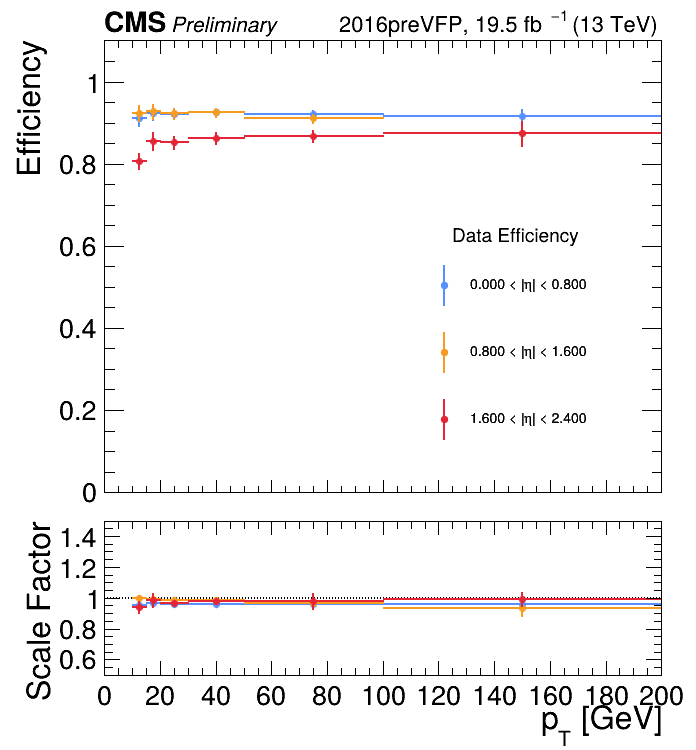
\includegraphics[width=0.45\textwidth]{Figures/analysis/Mu8El23_muon_eff_2016preVFP.png}}
  \hfill
  \subfloat[2016 postVFP]{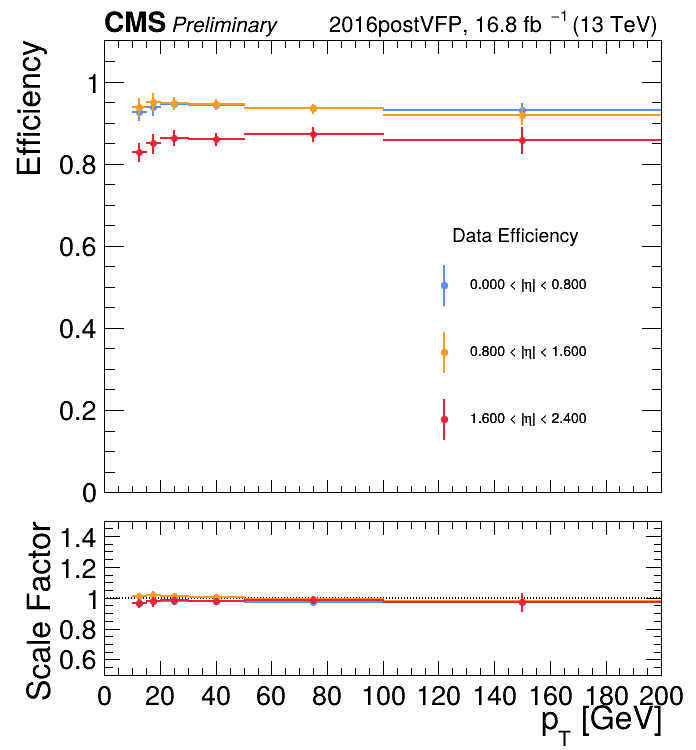
\includegraphics[width=0.45\textwidth]{Figures/analysis/Mu8El23_muon_eff_2016postVFP.png}} \\
  \subfloat[2017]{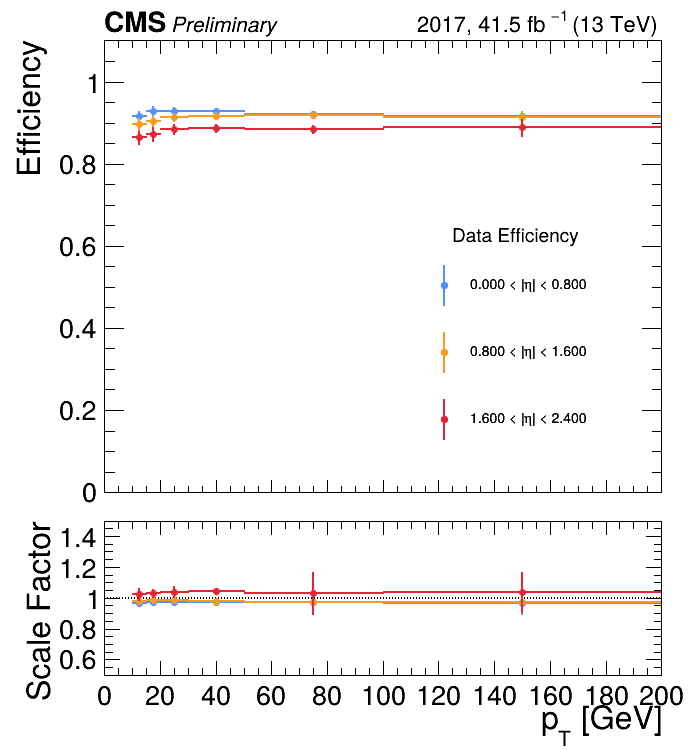
\includegraphics[width=0.45\textwidth]{Figures/analysis/Mu8El23_muon_eff_2017.png}}
  \hfill
  \subfloat[2018]{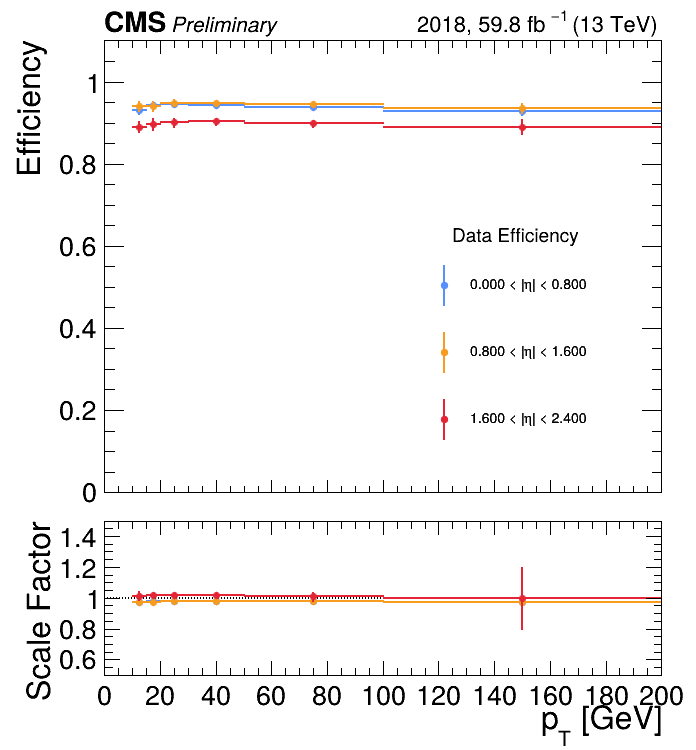
\includegraphics[width=0.45\textwidth]{Figures/analysis/Mu8El23_muon_eff_2018.png}}
  \caption{Muon leg ($\pT > 8\GeV$) efficiency for the \texttt{Mu8\_El23} cross-trigger as a function of muon $\pT$ in bins of $\eta$ for the Run~2 data-taking periods.}
  \label{fig:trig_mu8el23_mu_run2}
\end{figure}

\begin{figure}[htbp]
  \centering
  \subfloat[2022]{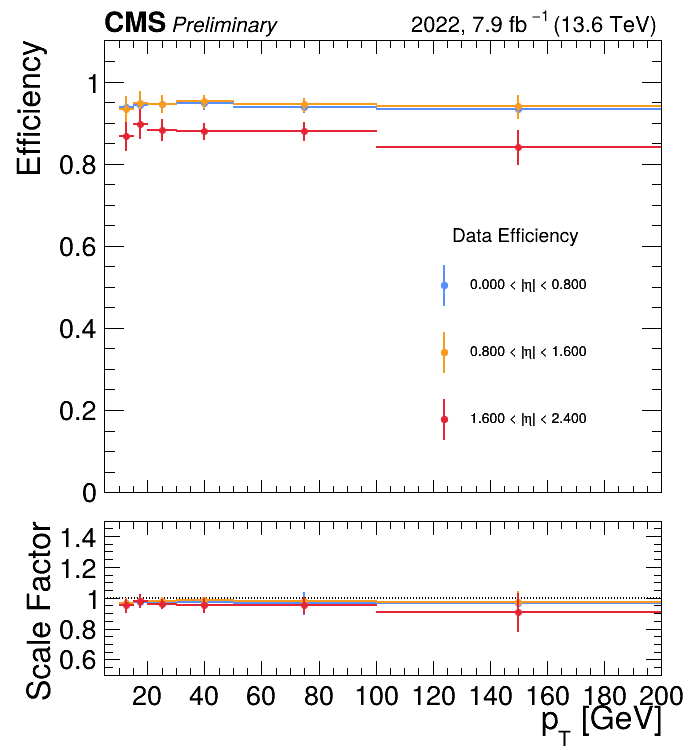
\includegraphics[width=0.45\textwidth]{Figures/analysis/Mu8El23_muon_eff_2022.png}}
  \hfill
  \subfloat[2022EE]{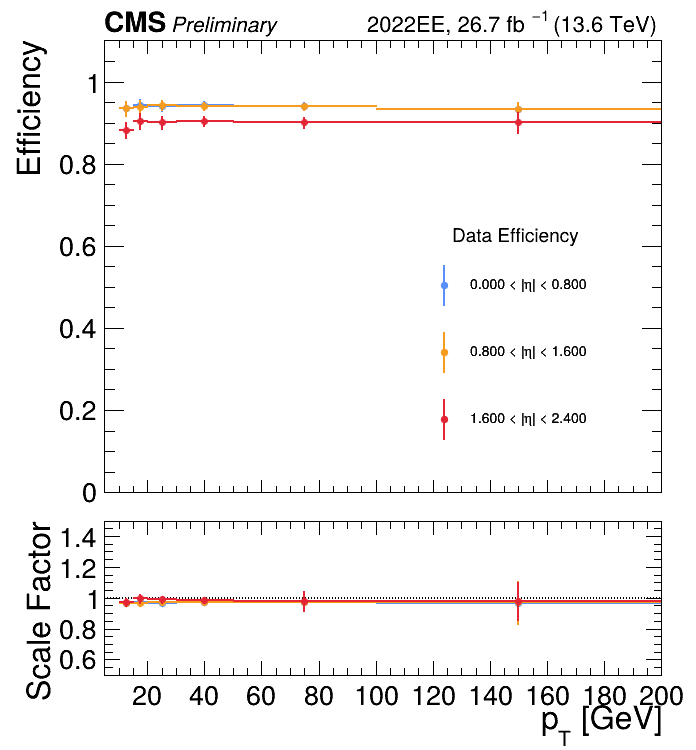
\includegraphics[width=0.45\textwidth]{Figures/analysis/Mu8El23_muon_eff_2022EE.png}} \\
  \subfloat[2023]{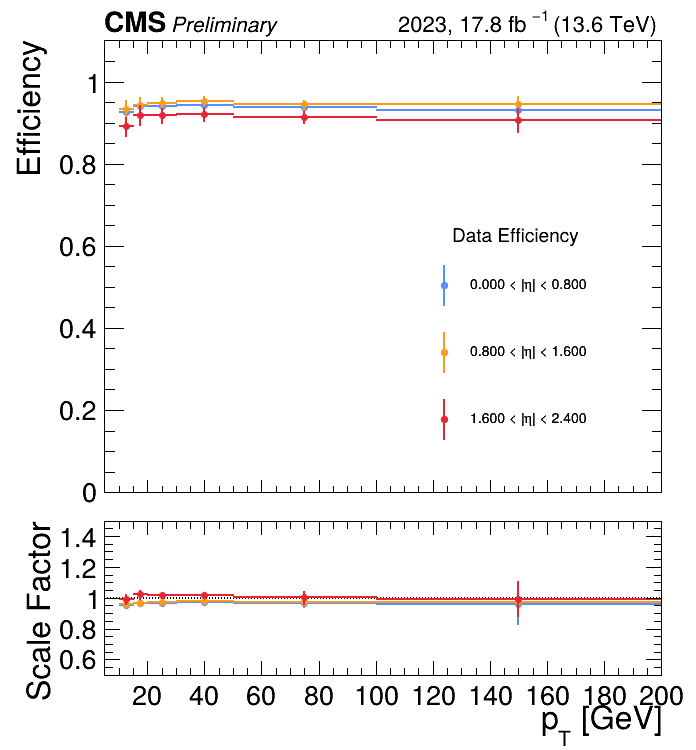
\includegraphics[width=0.45\textwidth]{Figures/analysis/Mu8El23_muon_eff_2023.png}}
  \hfill
  \subfloat[2023BPix]{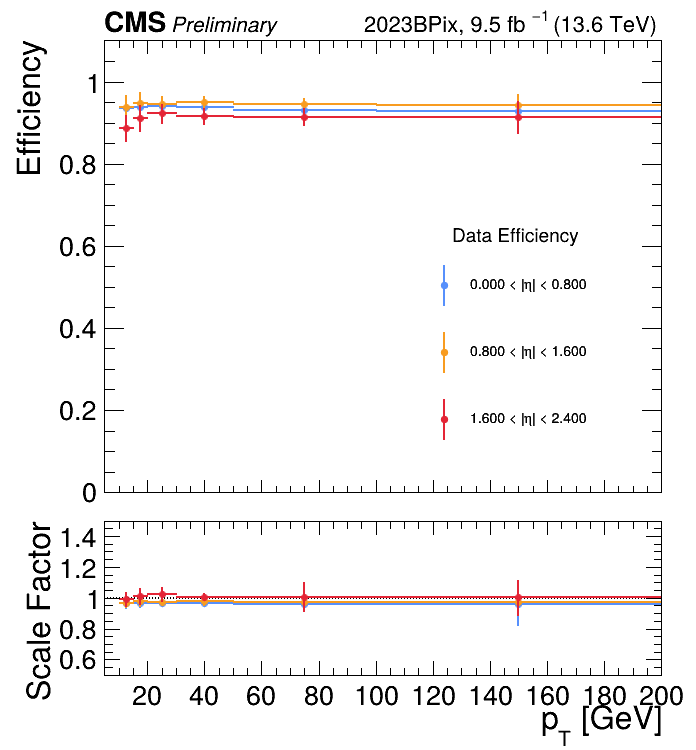
\includegraphics[width=0.45\textwidth]{Figures/analysis/Mu8El23_muon_eff_2023BPix.png}}
  \caption{Muon leg ($\pT > 8\GeV$) efficiency for the \texttt{Mu8\_El23} cross-trigger as a function of muon $\pT$ in bins of $\eta$ for the Run~3 data-taking periods.}
  \label{fig:trig_mu8el23_mu_run3}
\end{figure}

\begin{figure}[htbp]
  \centering
  \subfloat[2016 preVFP]{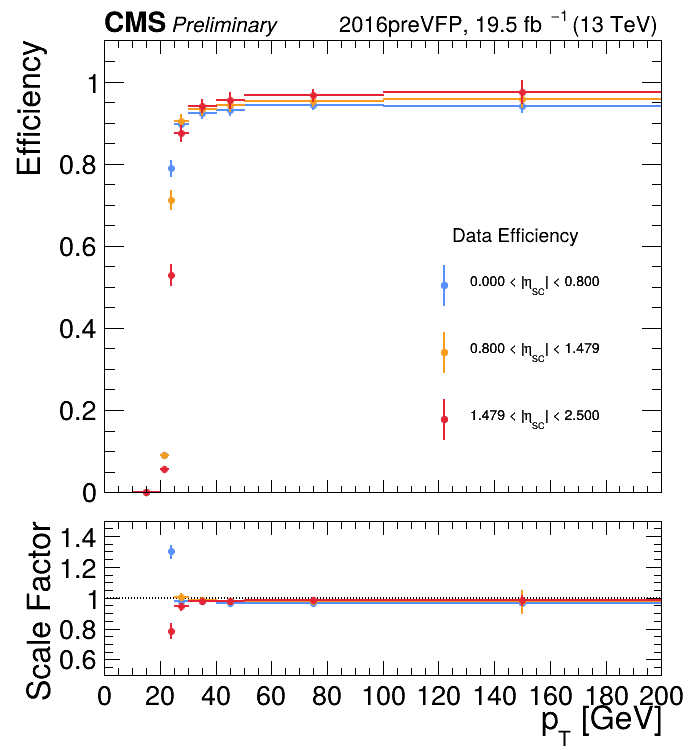
\includegraphics[width=0.45\textwidth]{Figures/analysis/Mu8El23_electron_eff_2016preVFP.png}}
  \hfill
  \subfloat[2016 postVFP]{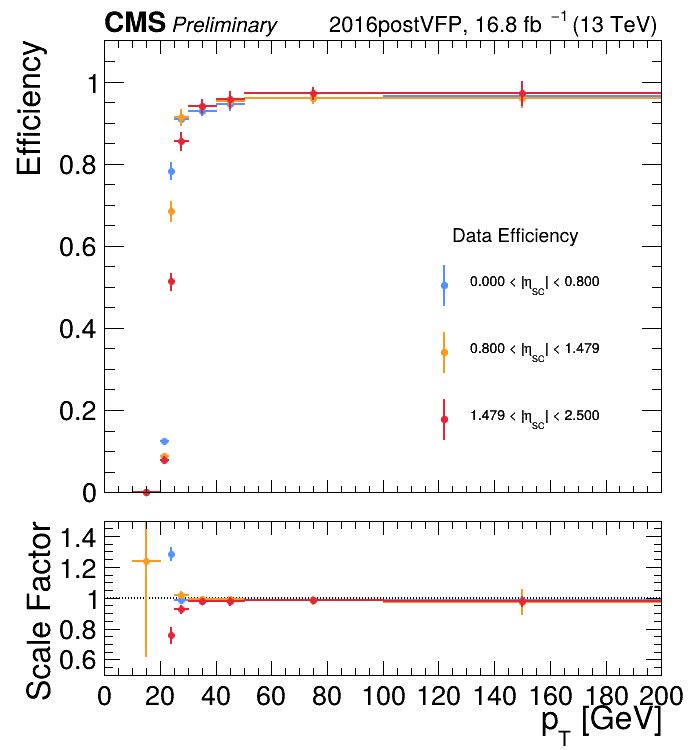
\includegraphics[width=0.45\textwidth]{Figures/analysis/Mu8El23_electron_eff_2016postVFP.png}} \\
  \subfloat[2017]{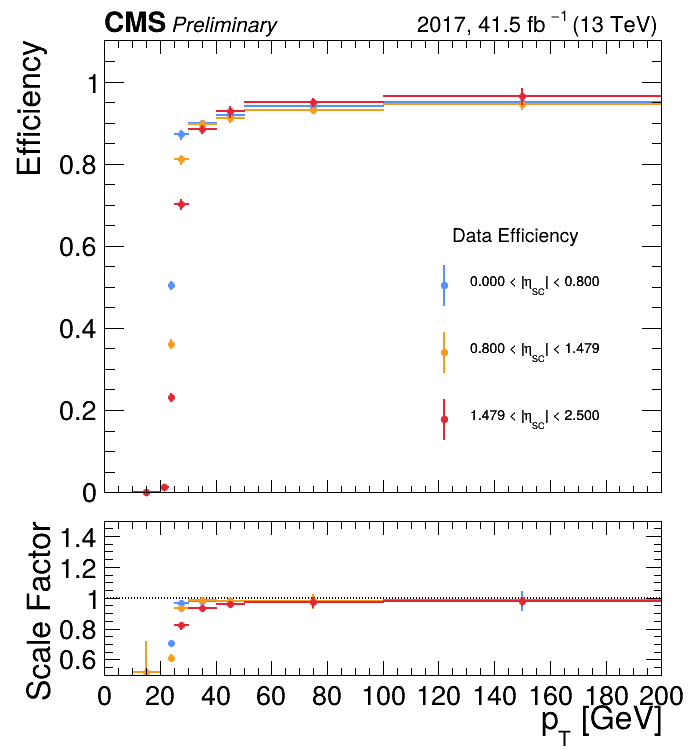
\includegraphics[width=0.45\textwidth]{Figures/analysis/Mu8El23_electron_eff_2017.png}}
  \hfill
  \subfloat[2018]{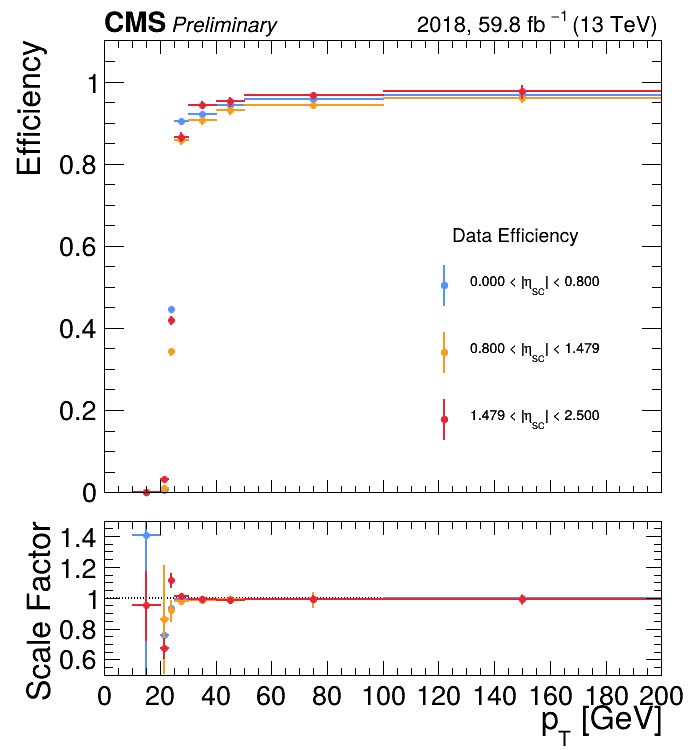
\includegraphics[width=0.45\textwidth]{Figures/analysis/Mu8El23_electron_eff_2018.png}}
  \caption{Electron leg ($\pT > 23\GeV$) efficiency for the \texttt{Mu8\_El23} cross-trigger as a function of electron $\pT$ in bins of $\eta_\text{SC}$ for the Run~2 data-taking periods.}
  \label{fig:trig_mu8el23_el_run2}
\end{figure}

\begin{figure}[htbp]
  \centering
  \subfloat[2022]{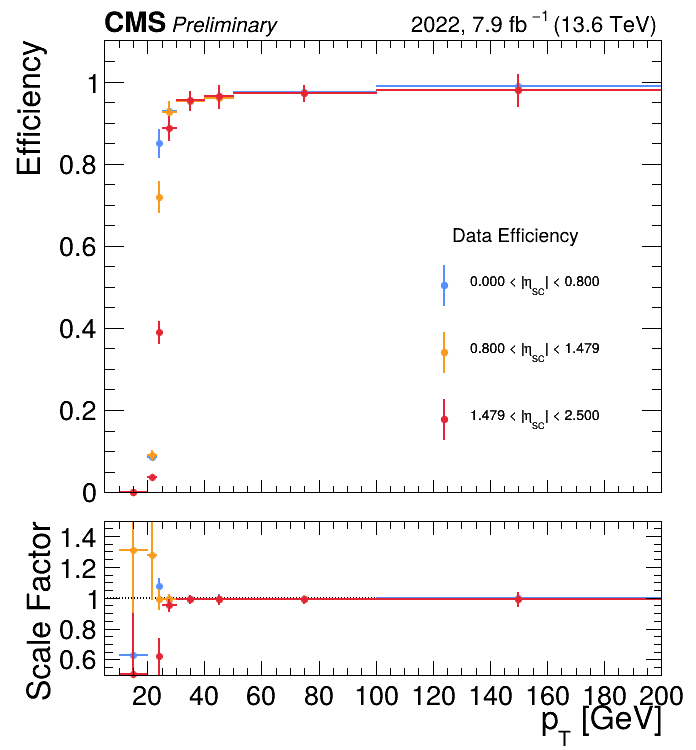
\includegraphics[width=0.45\textwidth]{Figures/analysis/Mu8El23_electron_eff_2022.png}}
  \hfill
  \subfloat[2022EE]{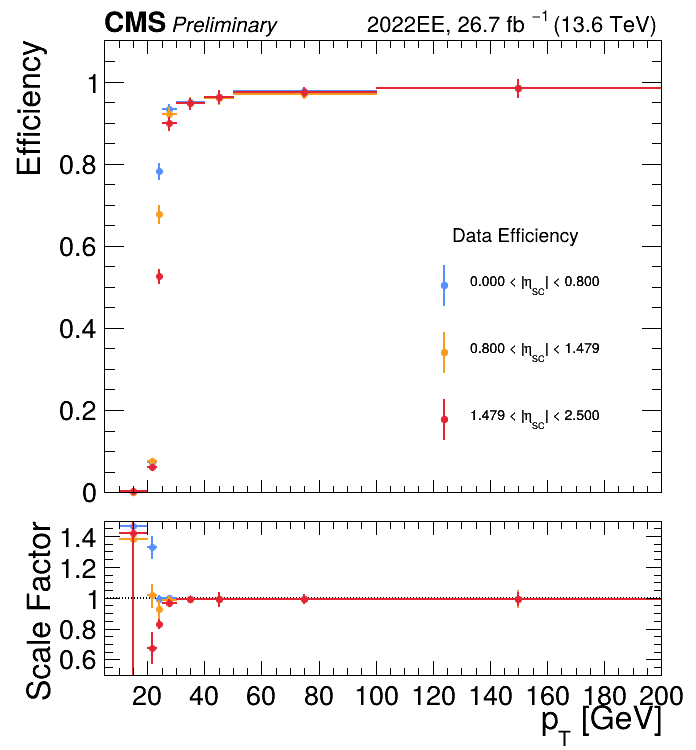
\includegraphics[width=0.45\textwidth]{Figures/analysis/Mu8El23_electron_eff_2022EE.png}} \\
  \subfloat[2023]{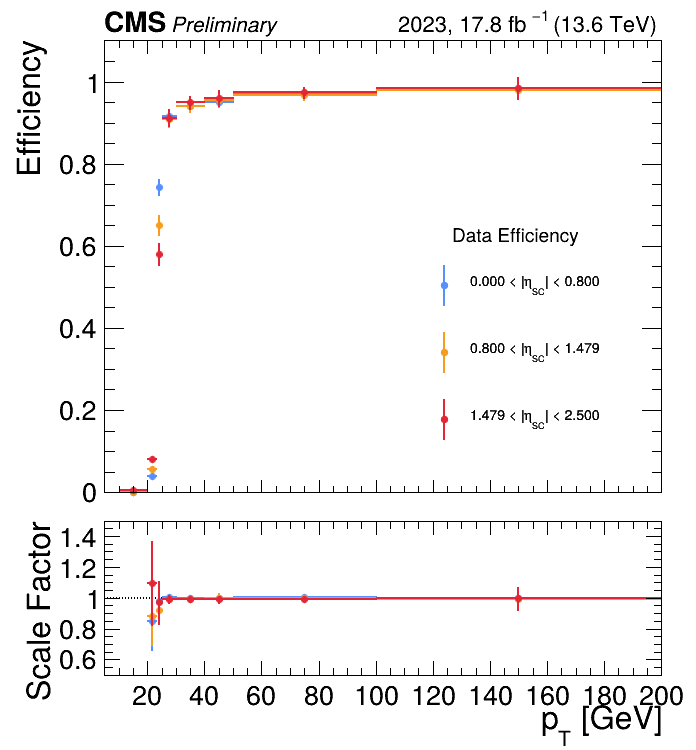
\includegraphics[width=0.45\textwidth]{Figures/analysis/Mu8El23_electron_eff_2023.png}}
  \hfill
  \subfloat[2023BPix]{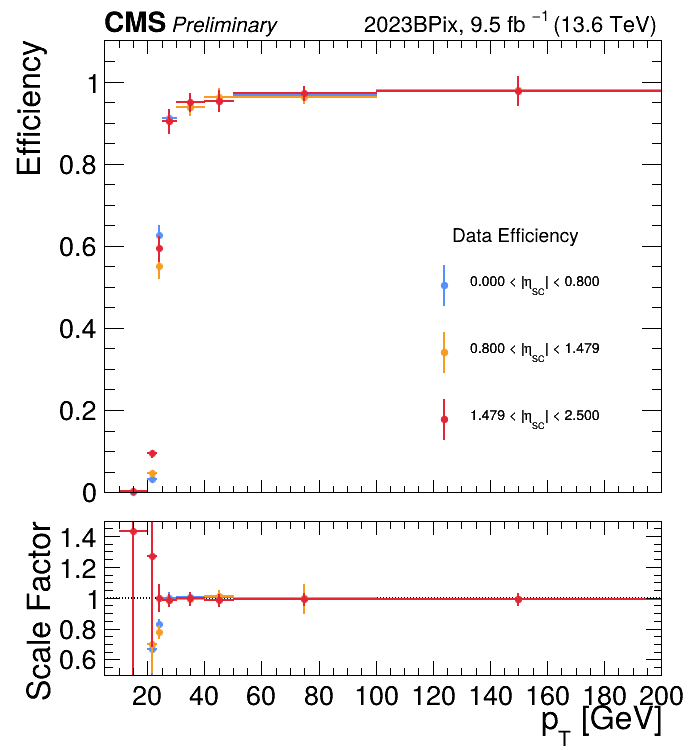
\includegraphics[width=0.45\textwidth]{Figures/analysis/Mu8El23_electron_eff_2023BPix.png}}
  \caption{Electron leg ($\pT > 23\GeV$) efficiency for the \texttt{Mu8\_El23} cross-trigger as a function of electron $\pT$ in bins of $\eta_\text{SC}$ for the Run~3 data-taking periods.}
  \label{fig:trig_mu8el23_el_run3}
\end{figure}

The pairwise filter efficiencies and their data-to-simulation scale factors are summarized in Tables~\ref{tab:pair_dimu} and~\ref{tab:pair_emu} for the dimuon and electron-muon triggers, respectively. In all cases the scale factors are consistent with unity at the sub-percent level.

\begin{table}[htbp]
\centering
\caption{Pairwise filter efficiency and data-to-simulation scale factor for dimuon triggers.}
\label{tab:pair_dimu}
\small
\begin{tabular}{llccc}
\hline\hline
Era & Filter & $\varepsilon_\text{data}$ & $\varepsilon_\text{MC}$ & SF \\
\hline
2016 postVFP & DZ            & $0.9798 \pm 0.0006$ & $0.9968 \pm 0.0005$ & $0.9829 \pm 0.0008$ \\
2017 (B)     & DZ            & $0.9956 \pm 0.0009$ & $0.9958 \pm 0.0004$ & $0.9998 \pm 0.0010$ \\
2017 (C--F)  & DZ\_Mass3p8   & $0.9962 \pm 0.0012$ & $0.9958 \pm 0.0004$ & $1.0004 \pm 0.0013$ \\
2018         & DZ\_Mass3p8   & $0.9988 \pm 0.0011$ & $0.9998 \pm 0.0004$ & $0.9990 \pm 0.0012$ \\
2022         & DZ\_Mass3p8   & $0.9996 \pm 0.0029$ & $0.9998 \pm 0.0035$ & $0.9998 \pm 0.0046$ \\
2022EE       & DZ\_Mass3p8   & $0.9994 \pm 0.0017$ & $0.9998 \pm 0.0019$ & $0.9996 \pm 0.0026$ \\
2023         & DZ\_Mass3p8   & $0.9993 \pm 0.0019$ & $0.9997 \pm 0.0025$ & $0.9996 \pm 0.0032$ \\
2023BPix     & DZ\_Mass3p8   & $0.9989 \pm 0.0026$ & $0.9996 \pm 0.0035$ & $0.9993 \pm 0.0044$ \\
\hline\hline
\end{tabular}
\end{table}

\begin{table}[htbp]
\centering
\caption{Pairwise filter efficiency and data-to-simulation scale factor for electron-muon triggers.}
\label{tab:pair_emu}
\small
\begin{tabular}{llccc}
\hline\hline
Era & Filter & $\varepsilon_\text{data}$ & $\varepsilon_\text{MC}$ & SF \\
\hline
2016 postVFP & DZ & $0.9638 \pm 0.0037$ & $0.9878 \pm 0.0007$ & $0.9757 \pm 0.0038$ \\
2017         & DZ & $0.9989 \pm 0.0023$ & $0.9955 \pm 0.0004$ & $1.0034 \pm 0.0023$ \\
2018         & DZ & $0.9946 \pm 0.0018$ & $0.9981 \pm 0.0004$ & $0.9965 \pm 0.0018$ \\
2022         & DZ & $0.9964 \pm 0.0048$ & $0.9985 \pm 0.0010$ & $0.9979 \pm 0.0049$ \\
2022EE       & DZ & $0.9949 \pm 0.0028$ & $0.9976 \pm 0.0006$ & $0.9973 \pm 0.0029$ \\
2023         & DZ & $0.9944 \pm 0.0032$ & $0.9977 \pm 0.0008$ & $0.9967 \pm 0.0033$ \\
2023BPix     & DZ & $0.9930 \pm 0.0044$ & $0.9972 \pm 0.0011$ & $0.9958 \pm 0.0045$ \\
\hline\hline
\end{tabular}
\end{table}

\subsubsection*{Jet energy corrections and b-tagging scale factors}

The JES and JER corrections described in Section~\ref{ssec:jets} use the latest calibrations provided by the JMET POG for each data-taking era. Systematic uncertainties are evaluated by varying the corrections within their uncertainties and propagating the effect to the final observable.

Flavor-dependent b-tagging scale factors from the BTV POG are applied on a per-jet basis using the fixed working point method (method 1a)~\cite{CMS:2017wtu}. The scale factors are derived from QCD multijet events and correct for differences in the b-tagging efficiency between data and simulation separately for b~quarks, c~quarks, and light-flavor jets.

\subsubsection*{Pileup reweighting}

The distribution of pileup interactions in simulation is reweighted to match the observed pileup profile in data, as described in Section~\ref{ssec:mc_samples}. The minimum bias cross section used in the pileup calculation is varied within its uncertainty to evaluate the associated systematic effect.

\subsection{Validation of object corrections}
\label{ssec:validation}

The combined effect of the object identification, trigger efficiency, jet energy, b-tagging, and pileup corrections described in the preceding subsections is validated in two dilepton control regions, chosen to probe the dominant physics objects in the analysis while remaining orthogonal to the trilepton signal region.

\subsubsection*{Inclusive dimuon control region}

An inclusive $\Pgm\Pgm$ sample is selected by requiring events to pass the dimuon triggers (Section~\ref{ssec:triggers}), contain exactly two opposite-charge muons satisfying the tight working point with $\pT > 20$ and $10\GeV$ for the leading and subleading muon, no additional loose leptons, and a dimuon invariant mass $m(\Pgm\Pgm) > 50\GeV$. This region is dominated by Drell--Yan production and validates the muon identification and isolation scale factors, the Rochester momentum corrections, the dimuon trigger efficiency, and the pileup reweighting.

The muon $\pT$ and $\eta$ distributions, the dimuon invariant mass, and the number of primary vertices are shown in Fig.~\ref{fig:dimu_cr}. The simulation, with all corrections applied, describes the data within the systematic uncertainty band across all kinematic variables.

\begin{figure}[p]
  \centering
  \subfloat{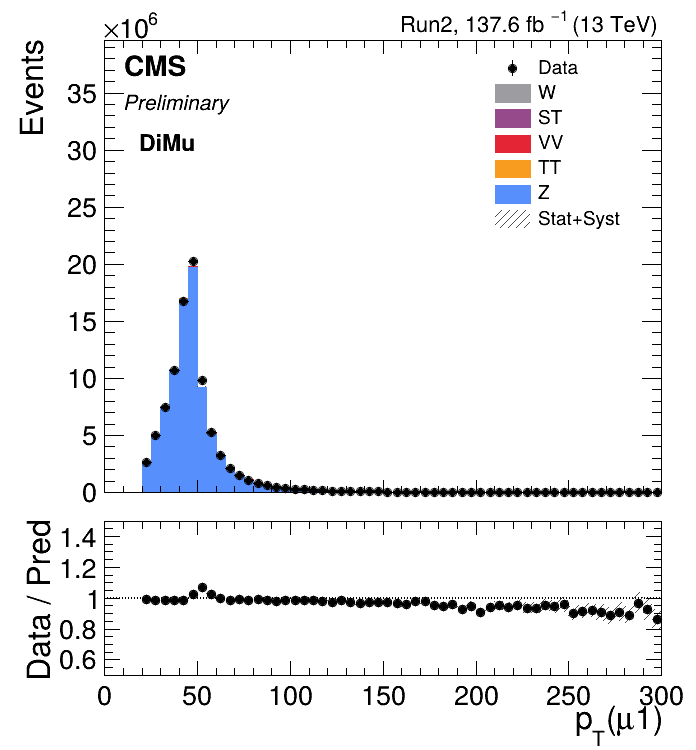
\includegraphics[width=0.32\textwidth]{Figures/analysis/DiMu_Run2_muons_1_pt.png}}
  \subfloat{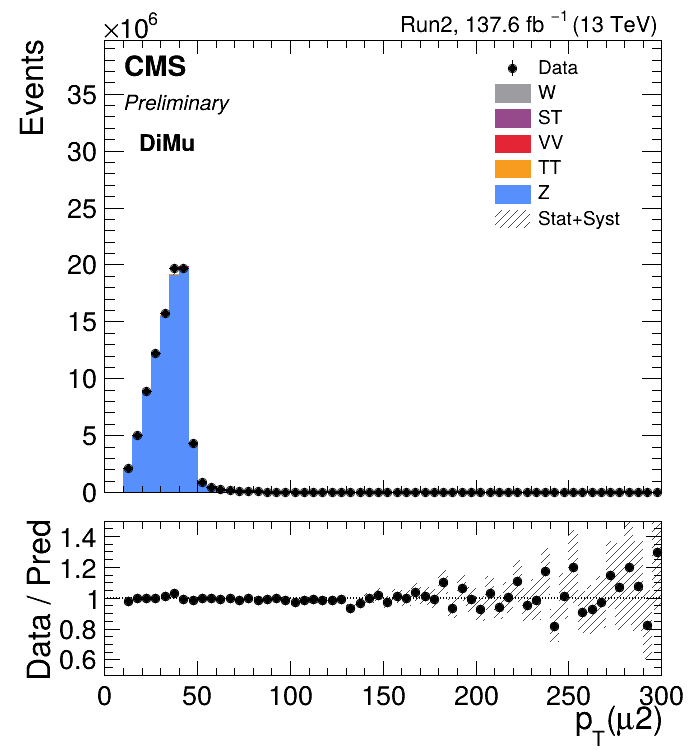
\includegraphics[width=0.32\textwidth]{Figures/analysis/DiMu_Run2_muons_2_pt.png}}
  \subfloat{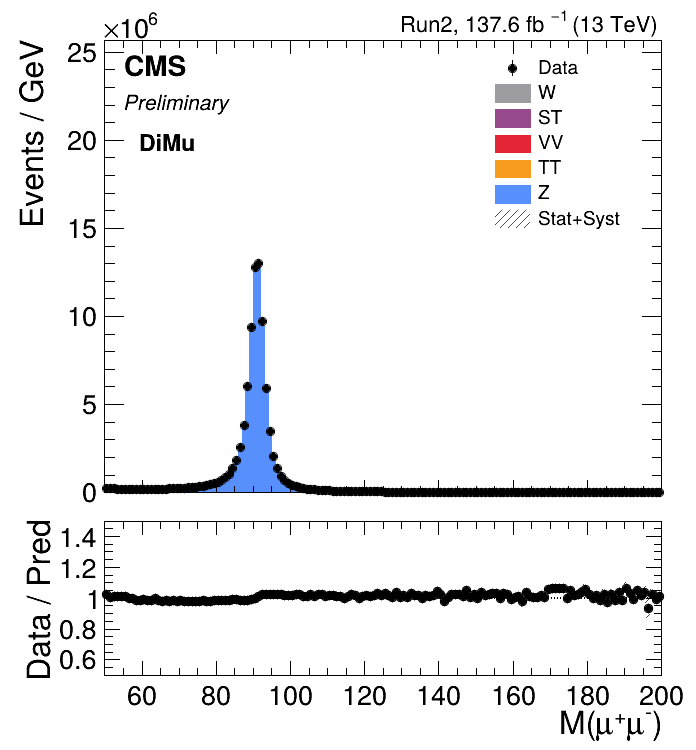
\includegraphics[width=0.32\textwidth]{Figures/analysis/DiMu_Run2_pair_mass.png}} \\
  \subfloat{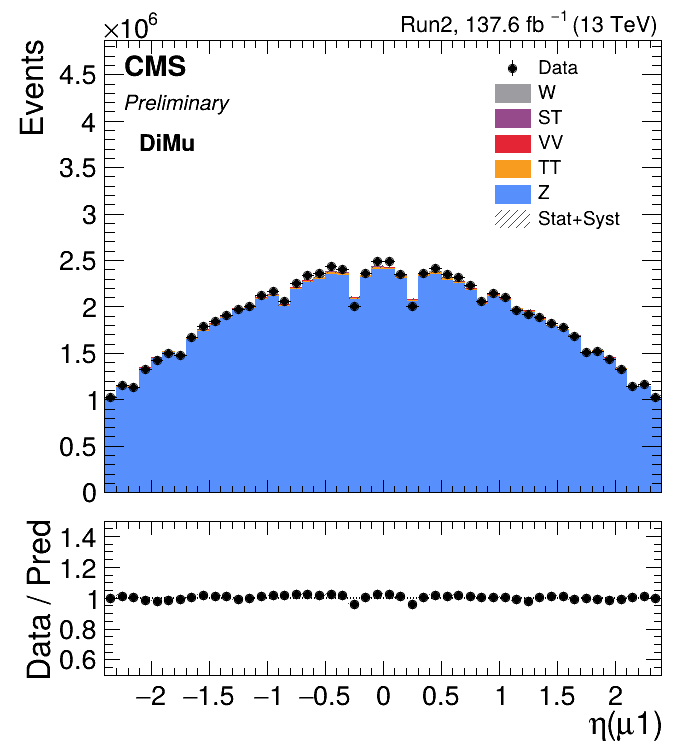
\includegraphics[width=0.32\textwidth]{Figures/analysis/DiMu_Run2_muons_1_eta.png}}
  \subfloat{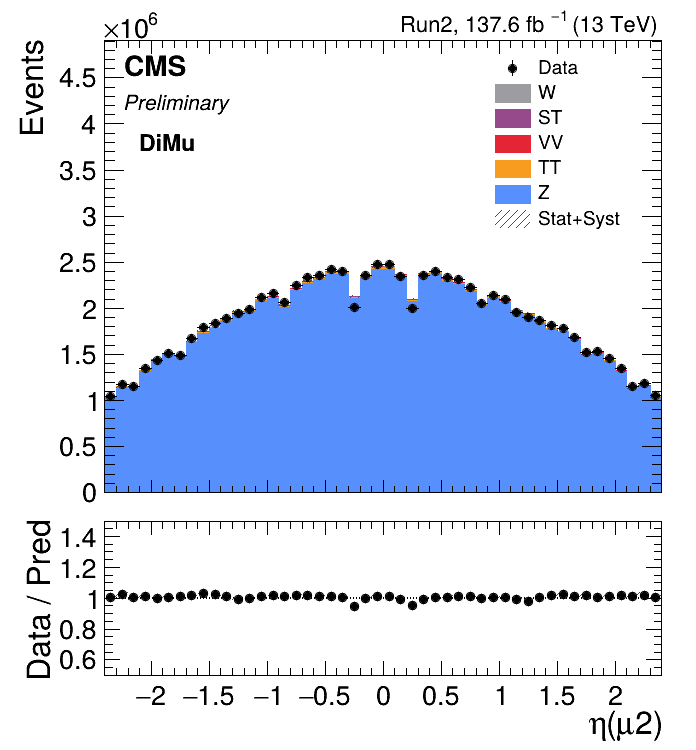
\includegraphics[width=0.32\textwidth]{Figures/analysis/DiMu_Run2_muons_2_eta.png}}
  \subfloat{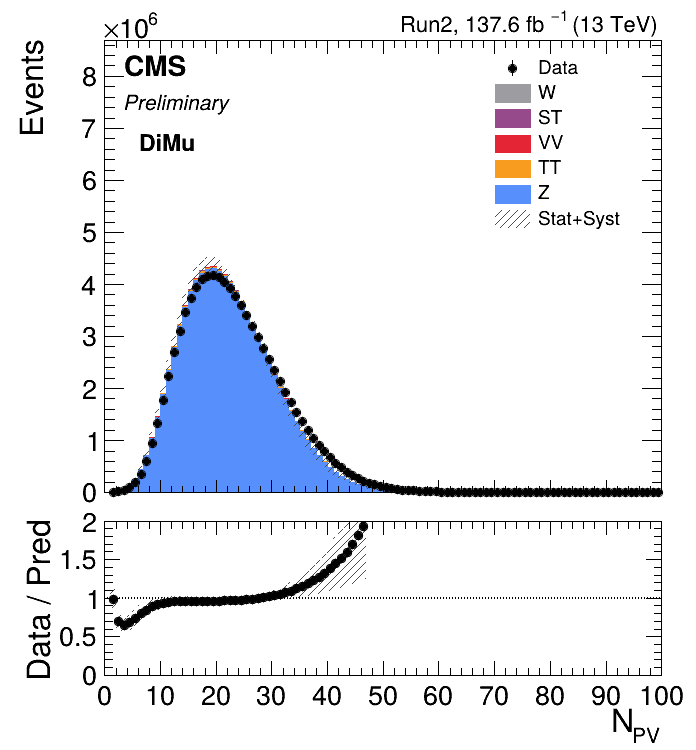
\includegraphics[width=0.32\textwidth]{Figures/analysis/DiMu_Run2_nPVsGood.png}} \\
  \subfloat{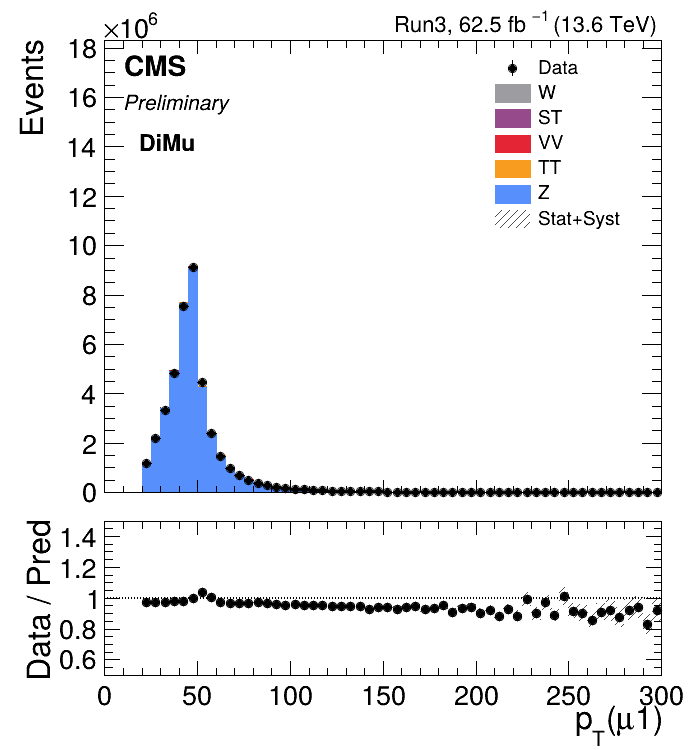
\includegraphics[width=0.32\textwidth]{Figures/analysis/DiMu_Run3_muons_1_pt.png}}
  \subfloat{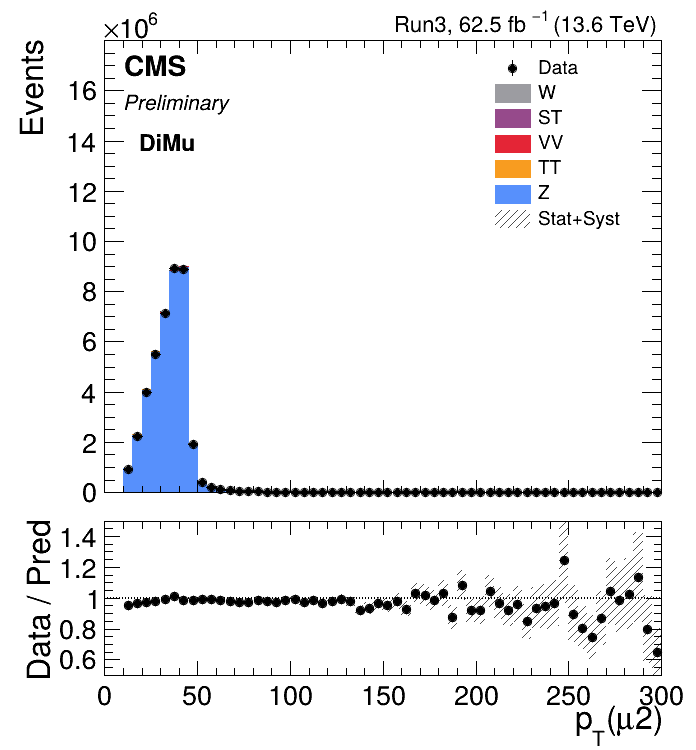
\includegraphics[width=0.32\textwidth]{Figures/analysis/DiMu_Run3_muons_2_pt.png}}
  \subfloat{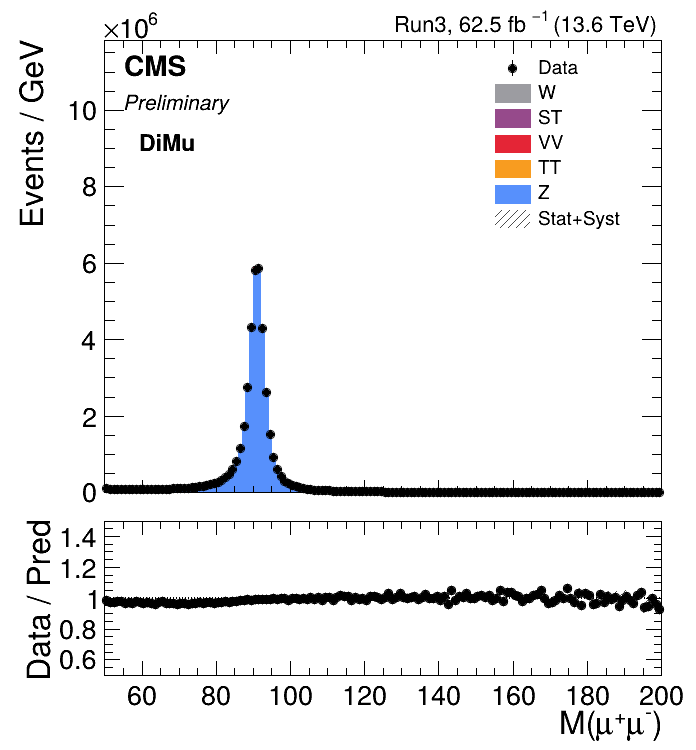
\includegraphics[width=0.32\textwidth]{Figures/analysis/DiMu_Run3_pair_mass.png}} \\
  \subfloat{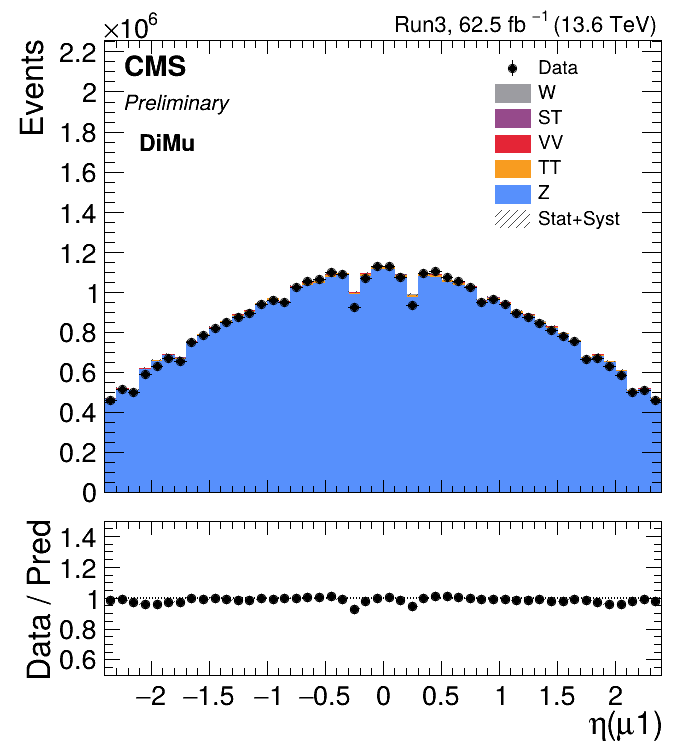
\includegraphics[width=0.32\textwidth]{Figures/analysis/DiMu_Run3_muons_1_eta.png}}
  \subfloat{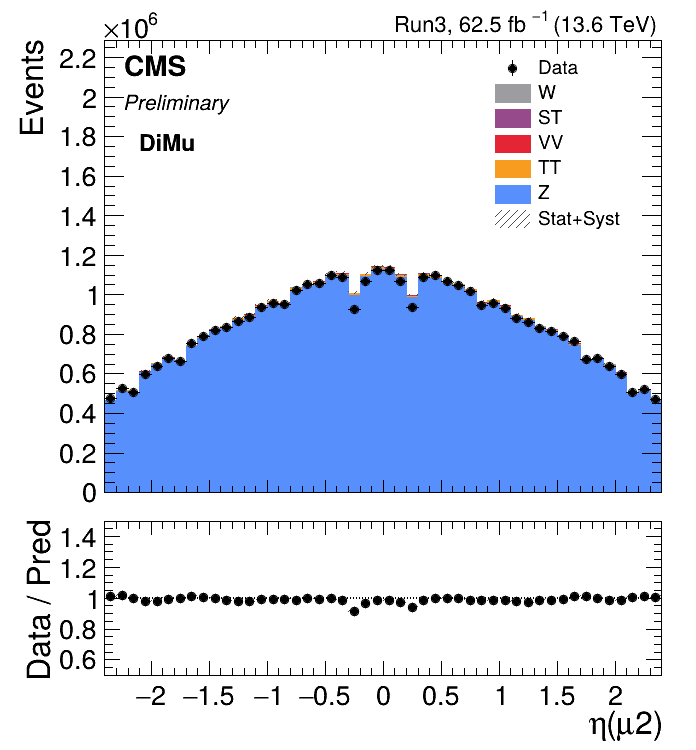
\includegraphics[width=0.32\textwidth]{Figures/analysis/DiMu_Run3_muons_2_eta.png}}
  \subfloat{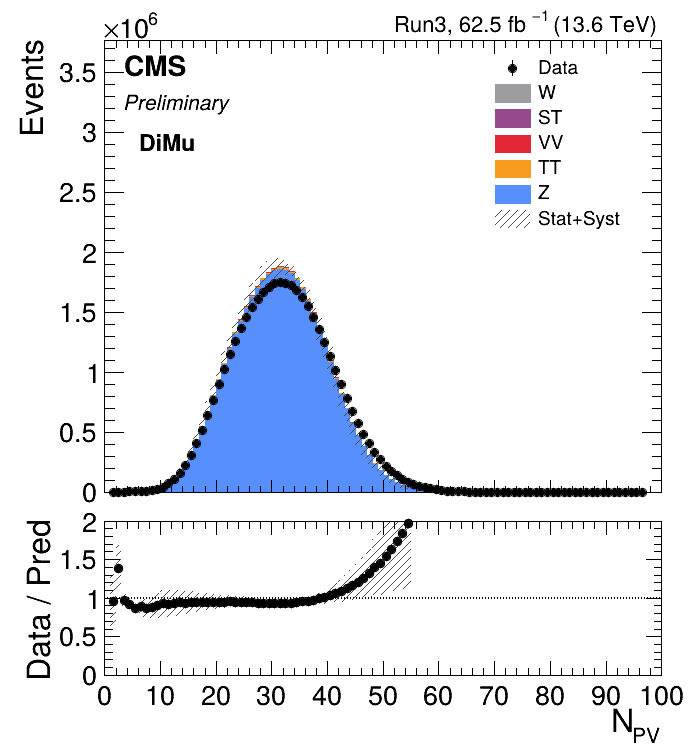
\includegraphics[width=0.32\textwidth]{Figures/analysis/DiMu_Run3_nPVsGood.png}}
  \caption{Distributions of the leading and subleading muon $\pT$ and $\eta$, the dimuon invariant mass, and the number of reconstructed primary vertices in the inclusive dimuon control region for Run~2 (rows~1--2) and Run~3 (rows~3--4). The hatched band represents the combined statistical and systematic uncertainty on the prediction.}
  \label{fig:dimu_cr}
\end{figure}

\subsubsection*{Top-enriched electron-muon control region}

A $\ttbar$-enriched $\Pe\Pgm$ sample is selected by requiring events to pass the electron-muon cross-triggers, contain exactly one opposite-charge electron-muon pair satisfying $\pT(\Pgm) > 25\GeV$ and $\pT(\Pe) > 15\GeV$, or $\pT(\Pgm) > 10\GeV$ and $\pT(\Pe) > 25\GeV$, with $\Delta R(\Pe, \Pgm) > 0.4$, no additional loose leptons, and at least two jets with at least one b-tagged jet. This region validates the electron identification and isolation scale factors, the electron-muon trigger efficiency, the jet energy corrections, and the b-tagging scale factors in a topology enriched in genuine $\ptmiss$ from $\PW$ boson decays.

The lepton $\pT$, $\eta$, $\ptmiss$, and pileup distributions are shown in Fig.~\ref{fig:emu_cr_lep}, and the jet and b-jet kinematic and multiplicity distributions in Fig.~\ref{fig:emu_cr_jet}. Good agreement between data and simulation is observed across all distributions for both Run~2 and Run~3.

\begin{figure}[p]
  \centering
  \subfloat{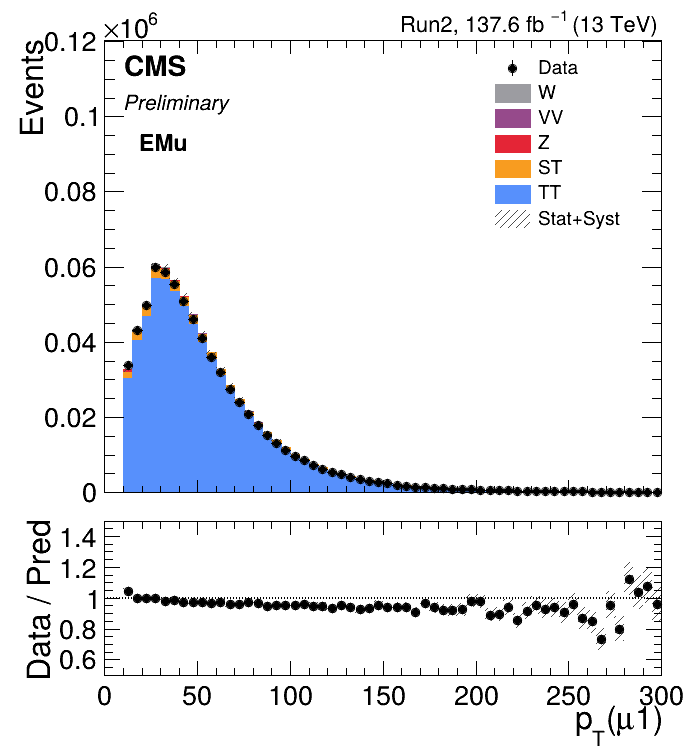
\includegraphics[width=0.32\textwidth]{Figures/analysis/EMu_Run2_muons_1_pt.png}}
  \subfloat{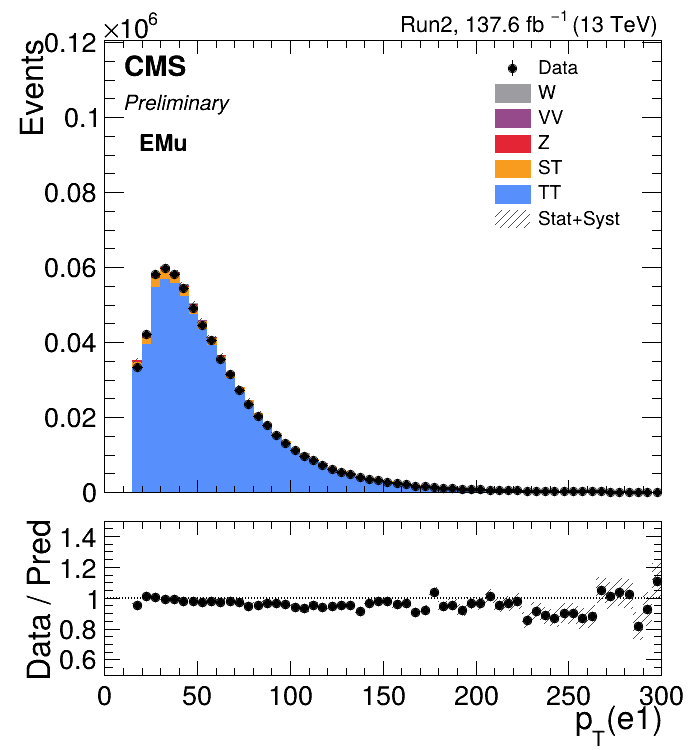
\includegraphics[width=0.32\textwidth]{Figures/analysis/EMu_Run2_electrons_1_pt.png}}
  \subfloat{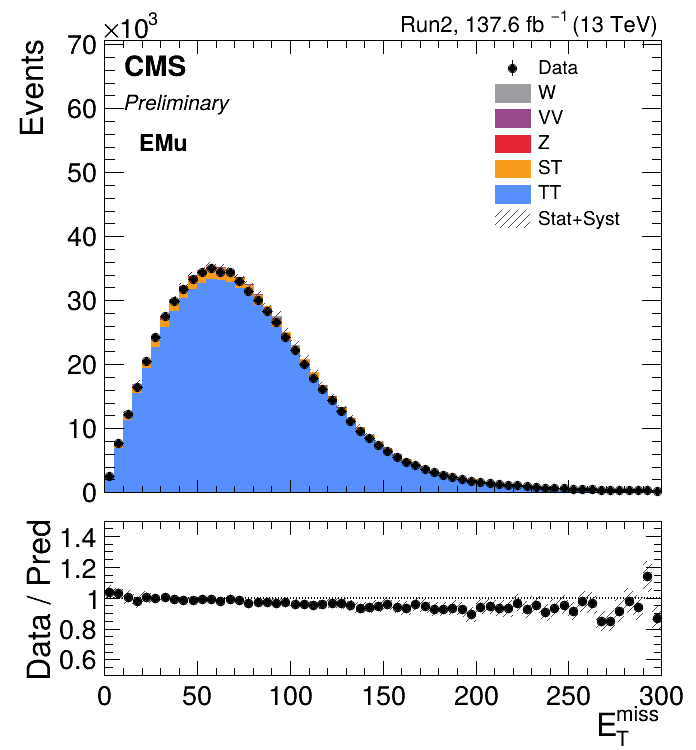
\includegraphics[width=0.32\textwidth]{Figures/analysis/EMu_Run2_METv_pt.png}} \\
  \subfloat{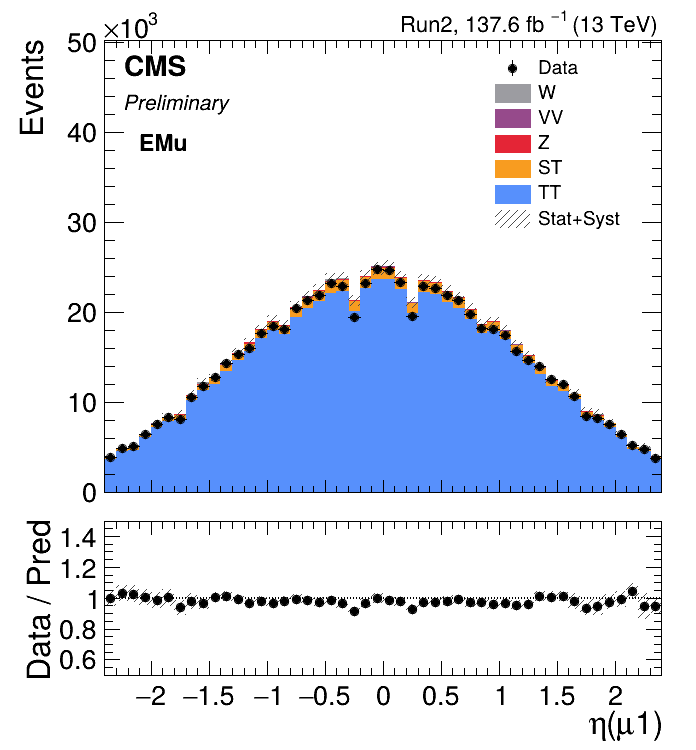
\includegraphics[width=0.32\textwidth]{Figures/analysis/EMu_Run2_muons_1_eta.png}}
  \subfloat{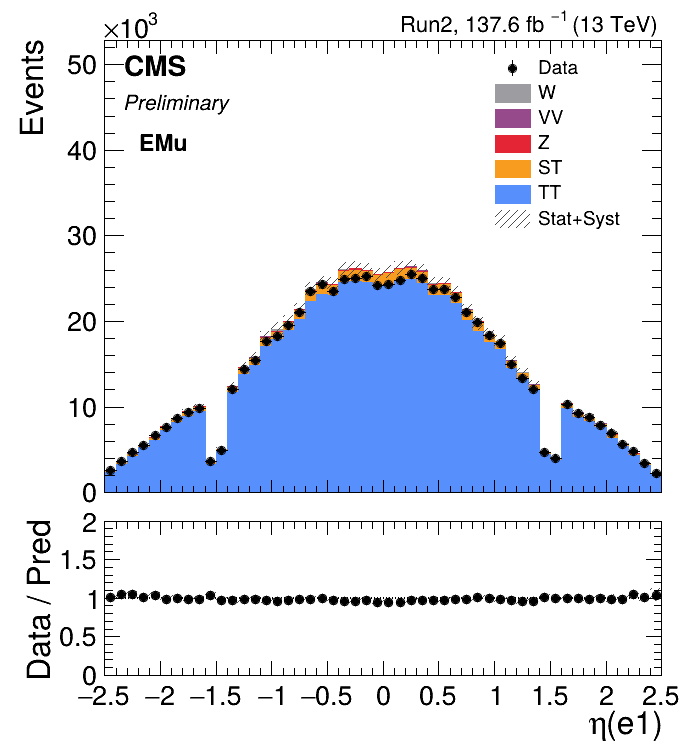
\includegraphics[width=0.32\textwidth]{Figures/analysis/EMu_Run2_electrons_1_eta.png}}
  \subfloat{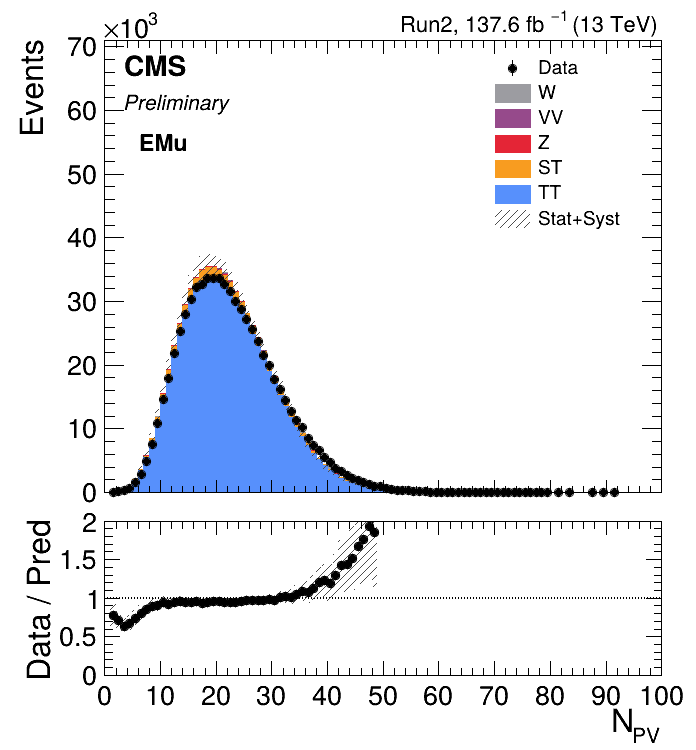
\includegraphics[width=0.32\textwidth]{Figures/analysis/EMu_Run2_nPVsGood.png}} \\
  \subfloat{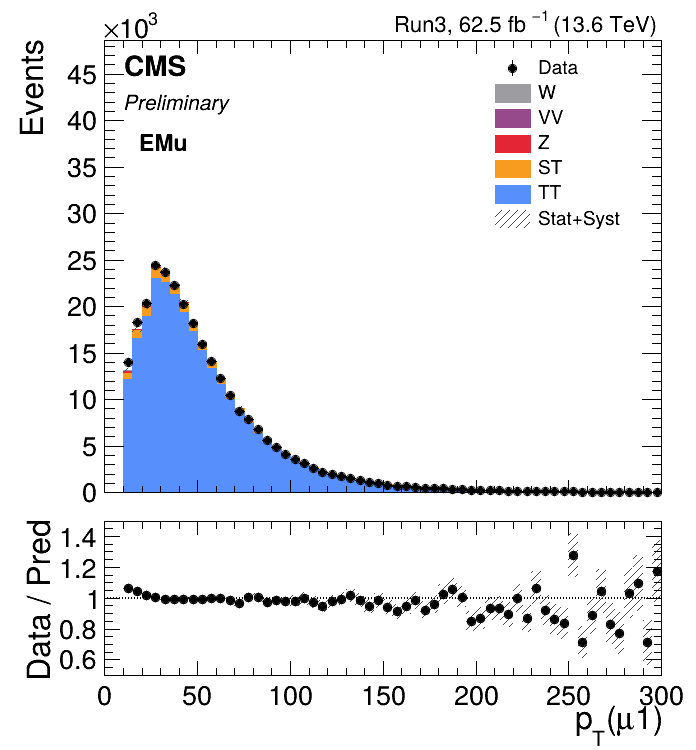
\includegraphics[width=0.32\textwidth]{Figures/analysis/EMu_Run3_muons_1_pt.png}}
  \subfloat{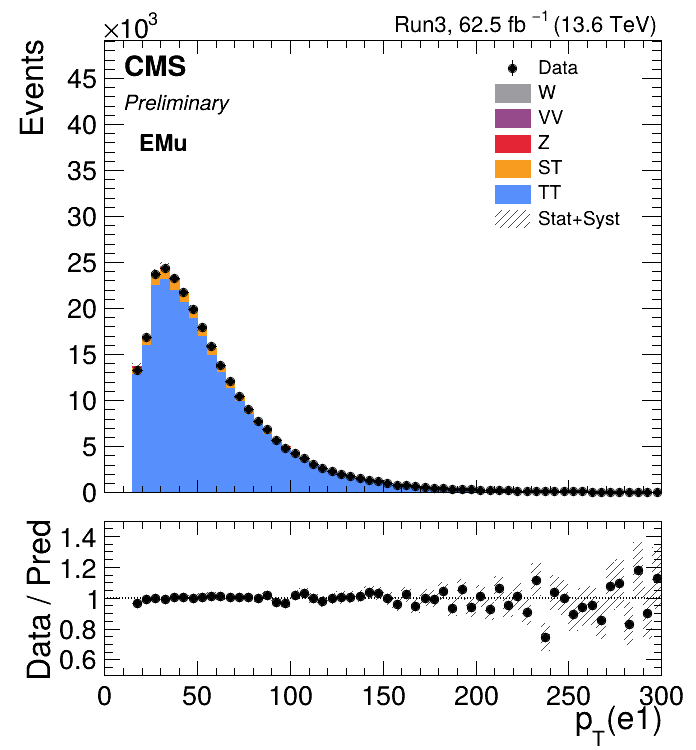
\includegraphics[width=0.32\textwidth]{Figures/analysis/EMu_Run3_electrons_1_pt.png}}
  \subfloat{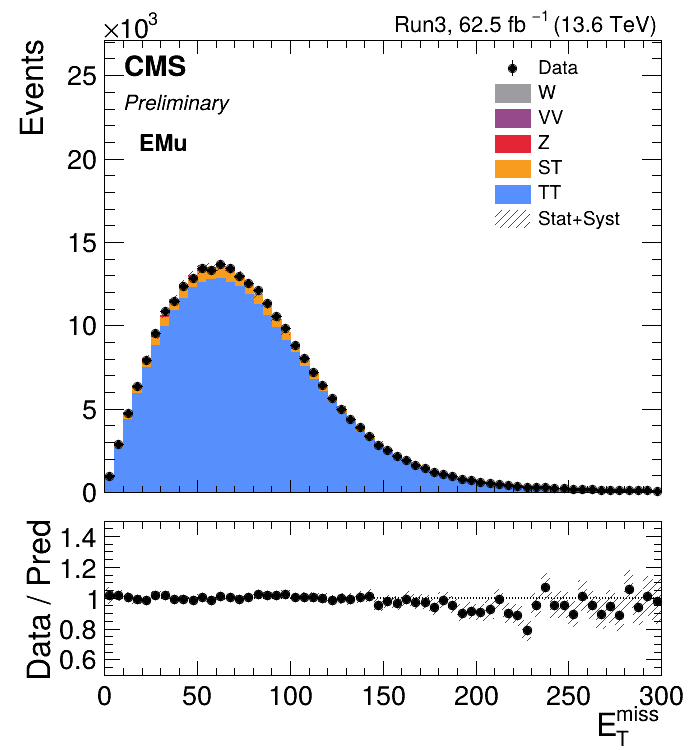
\includegraphics[width=0.32\textwidth]{Figures/analysis/EMu_Run3_METv_pt.png}} \\
  \subfloat{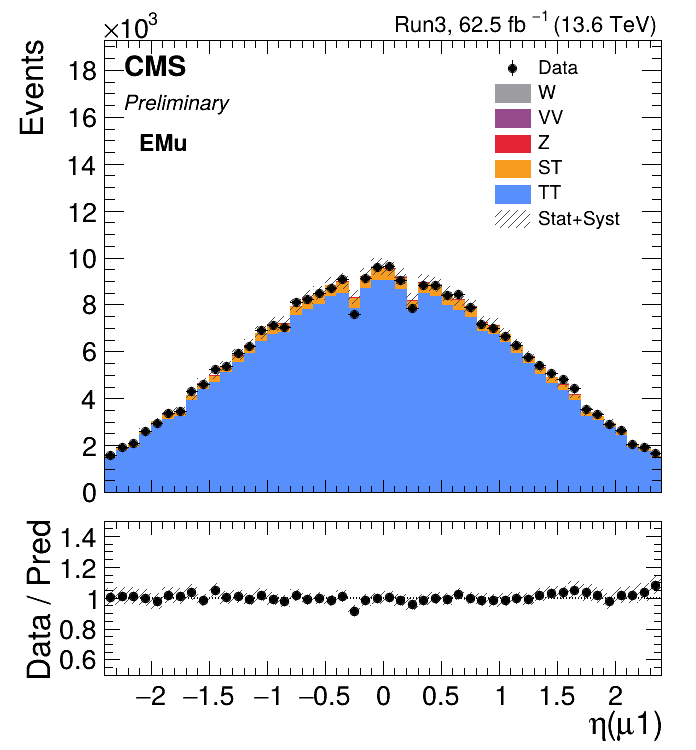
\includegraphics[width=0.32\textwidth]{Figures/analysis/EMu_Run3_muons_1_eta.png}}
  \subfloat{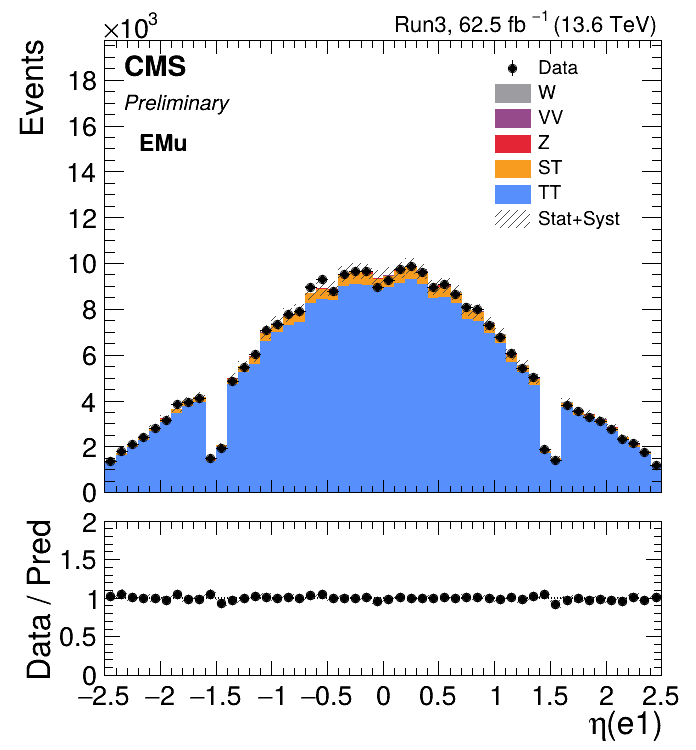
\includegraphics[width=0.32\textwidth]{Figures/analysis/EMu_Run3_electrons_1_eta.png}}
  \subfloat{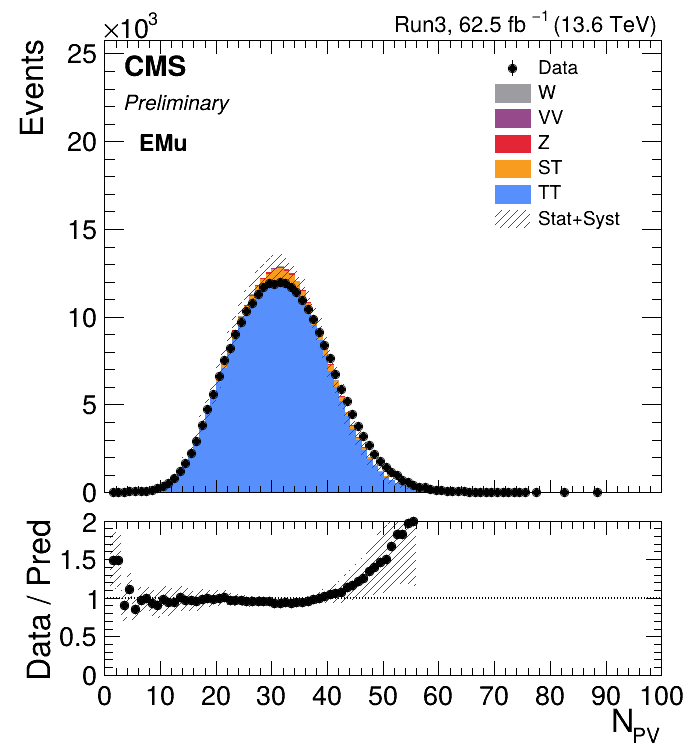
\includegraphics[width=0.32\textwidth]{Figures/analysis/EMu_Run3_nPVsGood.png}}
  \caption{Distributions of lepton $\pT$ and $\eta$, $\ptmiss$, and the number of reconstructed primary vertices in the top-enriched $\Pe\Pgm$ control region for Run~2 (rows~1--2) and Run~3 (rows~3--4).}
  \label{fig:emu_cr_lep}
\end{figure}

\begin{figure}[p]
  \centering
  \subfloat{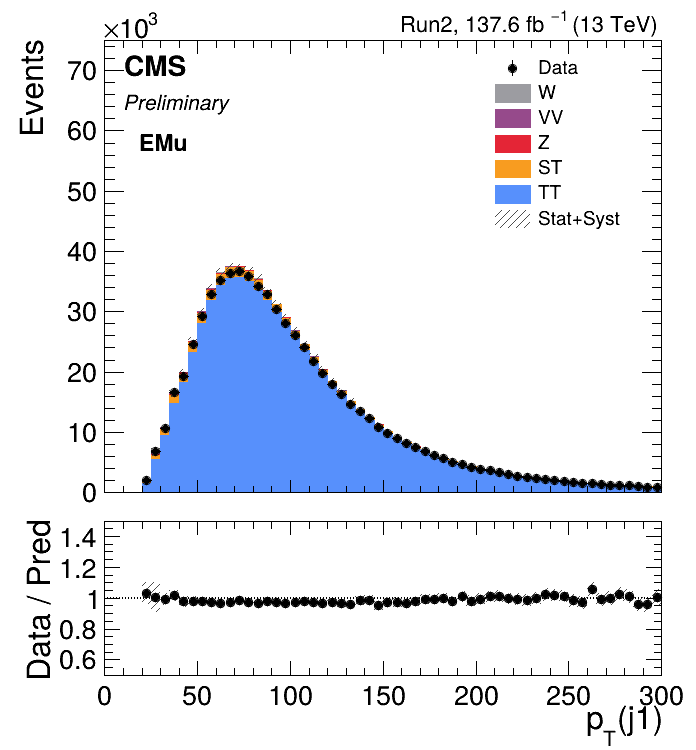
\includegraphics[width=0.32\textwidth]{Figures/analysis/EMu_Run2_jets_1_pt.png}}
  \subfloat{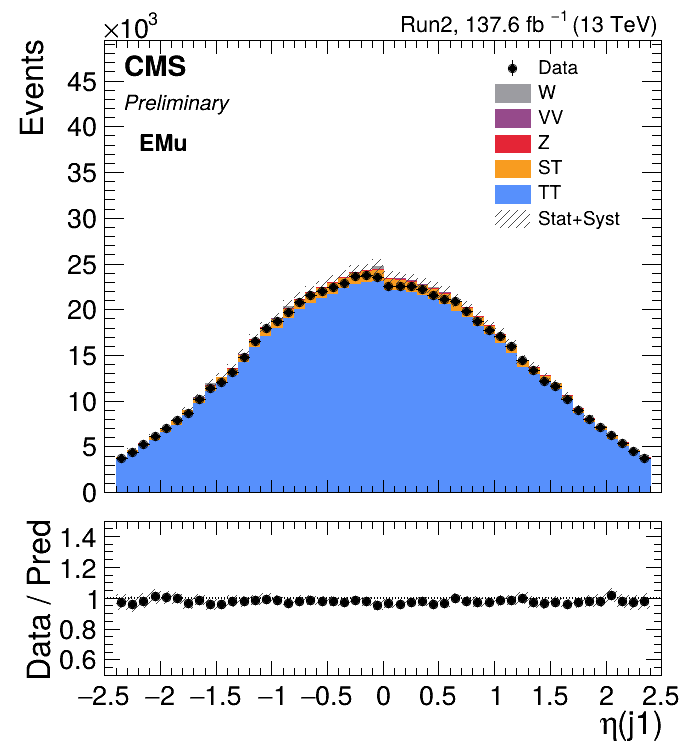
\includegraphics[width=0.32\textwidth]{Figures/analysis/EMu_Run2_jets_1_eta.png}}
  \subfloat{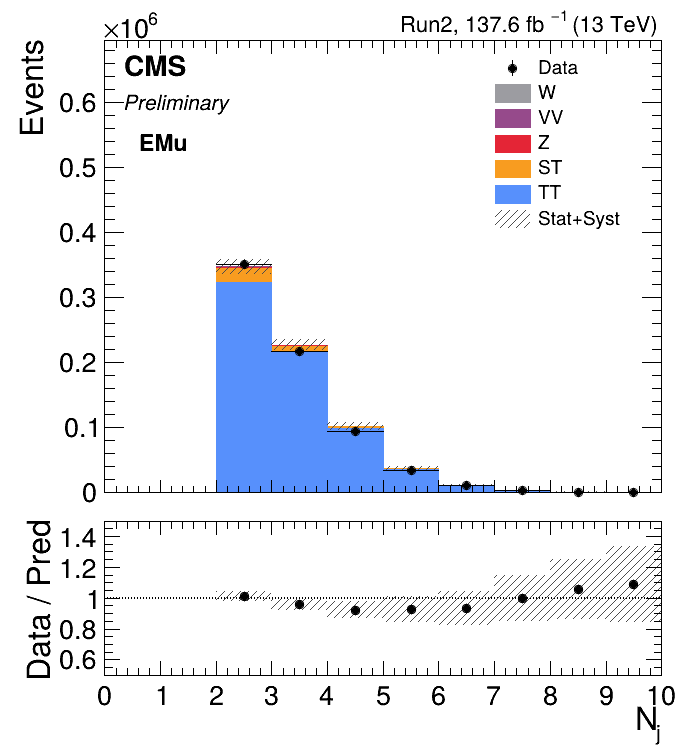
\includegraphics[width=0.32\textwidth]{Figures/analysis/EMu_Run2_jets_size.png}} \\
  \subfloat{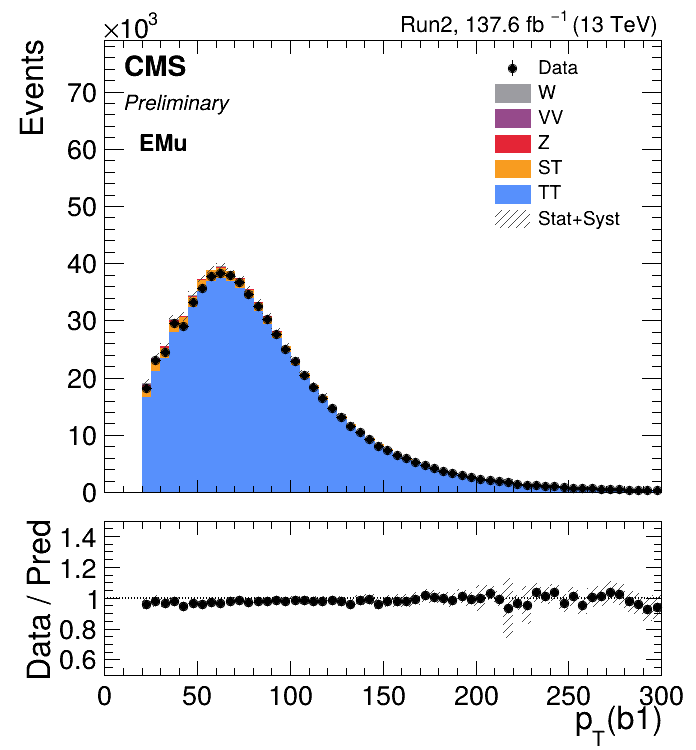
\includegraphics[width=0.32\textwidth]{Figures/analysis/EMu_Run2_bjets_1_pt.png}}
  \subfloat{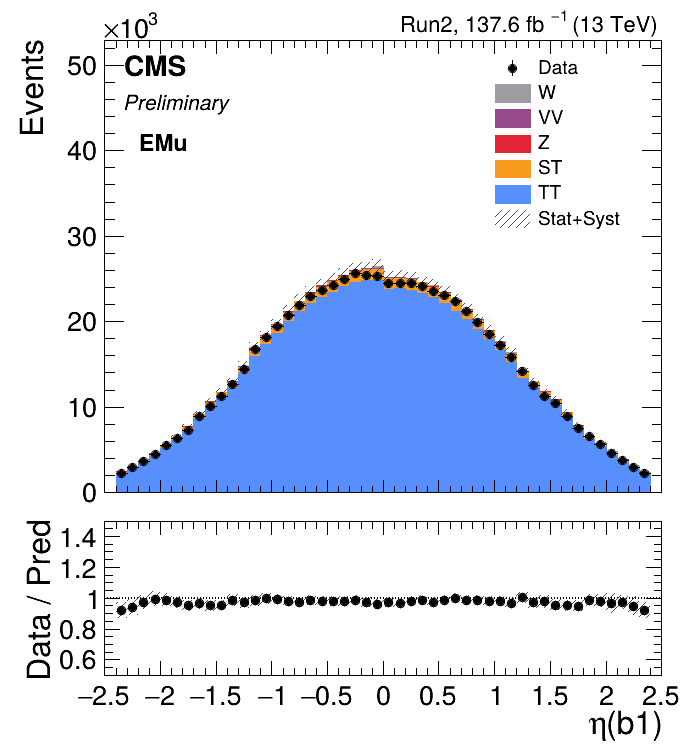
\includegraphics[width=0.32\textwidth]{Figures/analysis/EMu_Run2_bjets_1_eta.png}}
  \subfloat{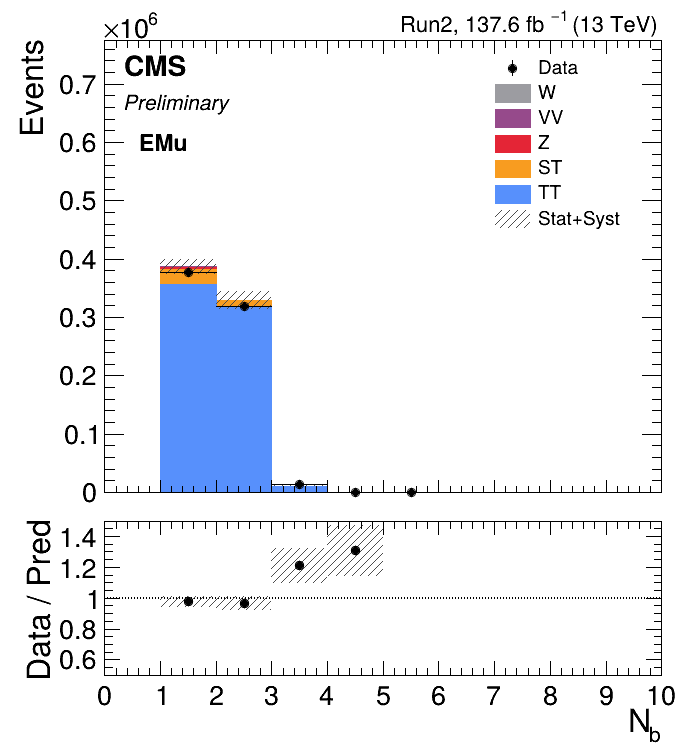
\includegraphics[width=0.32\textwidth]{Figures/analysis/EMu_Run2_bjets_size.png}} \\
  \subfloat{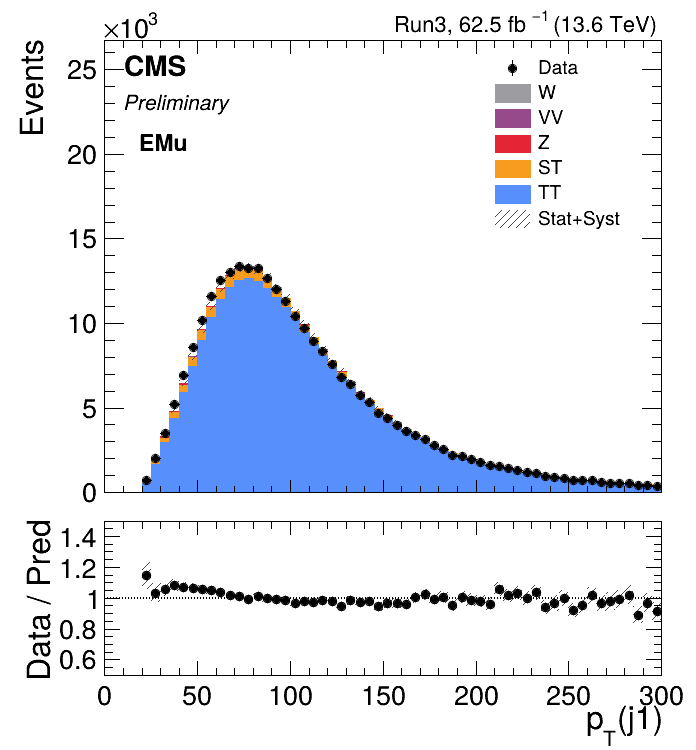
\includegraphics[width=0.32\textwidth]{Figures/analysis/EMu_Run3_jets_1_pt.png}}
  \subfloat{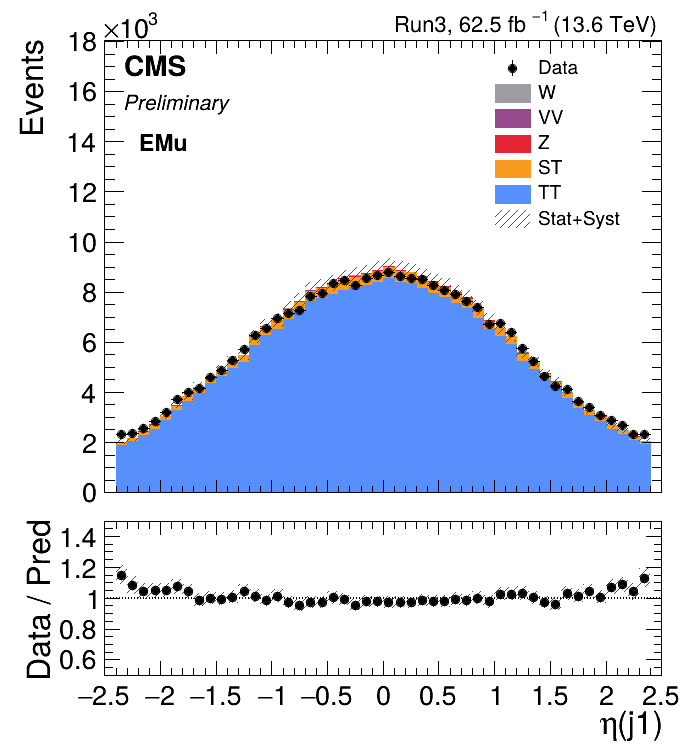
\includegraphics[width=0.32\textwidth]{Figures/analysis/EMu_Run3_jets_1_eta.png}}
  \subfloat{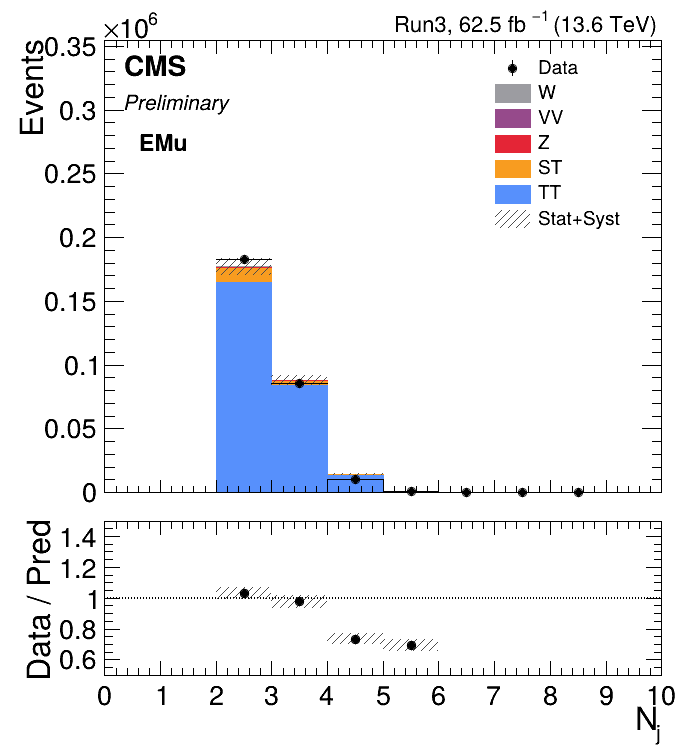
\includegraphics[width=0.32\textwidth]{Figures/analysis/EMu_Run3_jets_size.png}} \\
  \subfloat{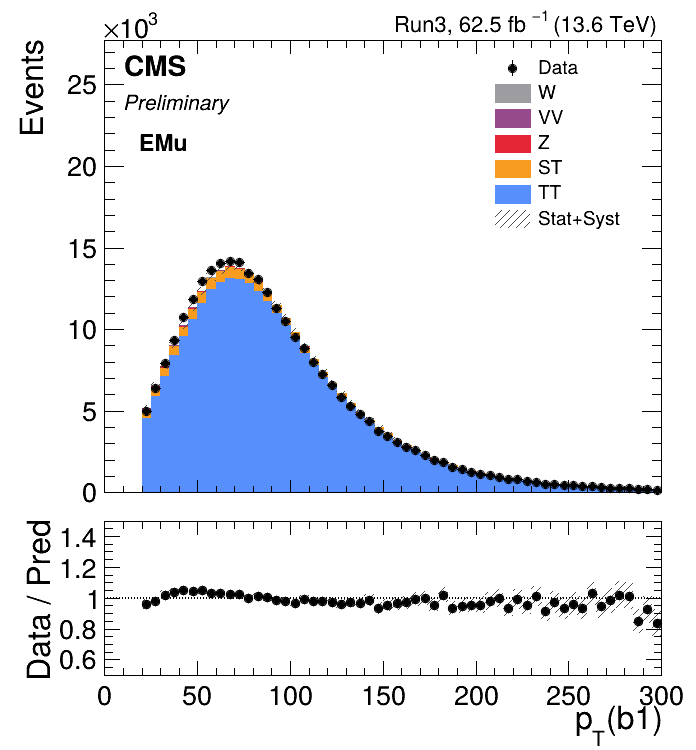
\includegraphics[width=0.32\textwidth]{Figures/analysis/EMu_Run3_bjets_1_pt.png}}
  \subfloat{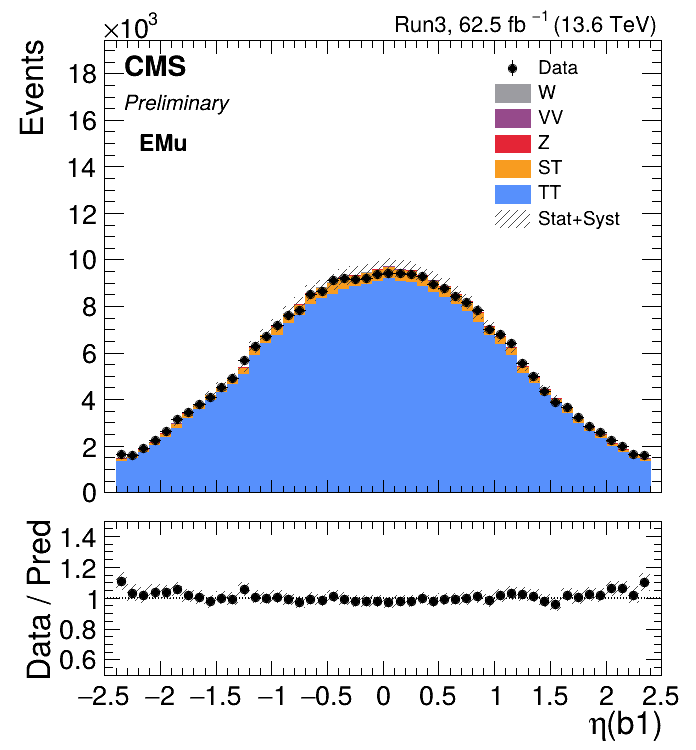
\includegraphics[width=0.32\textwidth]{Figures/analysis/EMu_Run3_bjets_1_eta.png}}
  \subfloat{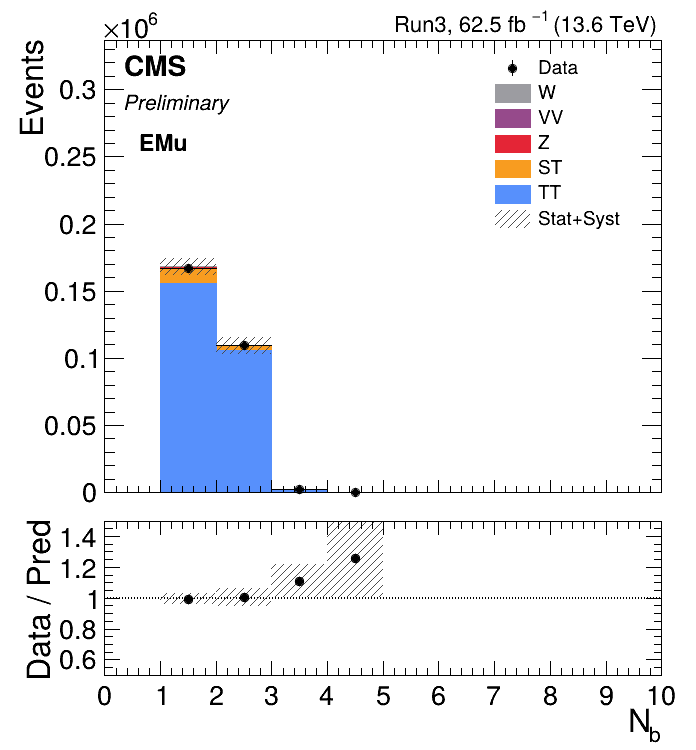
\includegraphics[width=0.32\textwidth]{Figures/analysis/EMu_Run3_bjets_size.png}}
  \caption{Distributions of leading jet and leading b-tagged jet $\pT$, $\eta$, and multiplicity in the top-enriched $\Pe\Pgm$ control region for Run~2 (rows~1--2) and Run~3 (rows~3--4).}
  \label{fig:emu_cr_jet}
\end{figure}

%% ============================================================
\section{Signal Extraction Strategy}
\label{sec:signal_extraction}
%% ============================================================

\subsection{Baseline Event Selection}
\label{ssec:baseline_selection}

The baseline selection isolates the trilepton final state from the $\PHc \to \PW^\pm \PA \to \PW^\pm \Pgm\Pgm$ decay chain while suppressing diboson, Drell--Yan, and $\ttbar$-associated backgrounds. The key requirements are:

\begin{itemize}
\item \textbf{Lepton multiplicity}: exactly three leptons passing tight identification, with one opposite-sign (OS) muon pair, in either $\Pe\Pgm\Pgm$ or $\Pgm\Pgm\Pgm$ configurations. Events containing additional leptons passing loose identification are vetoed.
\item \textbf{Lepton \pT thresholds}: $\pT(\Pe) > 15\GeV$, $\pT(\Pgm) > 10\GeV$, with trigger-safe requirements of $\pT > 25\GeV$ on the leading lepton in each channel.
\item \textbf{OS dimuon invariant mass}: each OS muon pair must satisfy $m(\Pgm^+\Pgm^-) > 12\GeV$ to suppress backgrounds from low-mass resonances such as $\PJGy$ and $\PgU$.
\item \textbf{Jet requirements}: at least two jets ($N_j \geq 2$) and at least one b-tagged jet ($N_b \geq 1$) are required. These requirements effectively suppress diboson and Drell--Yan backgrounds, which typically produce fewer jets and rarely contain b~quarks, while retaining the $\ttbar$-associated signal topology.
\end{itemize}

Figures~\ref{fig:baseline_emumu} and~\ref{fig:baseline_mumumu} show the OS dimuon invariant mass, jet multiplicity, and b-tagged jet multiplicity after the baseline selection for representative signal mass hypotheses and the dominant background processes. Signal distributions for $(\mHc, \mA)$ values of $(70, 15)$, $(100, 60)$, $(130, 90)$, and $(160, 155)\GeV$ illustrate the range of kinematic configurations. A clear signal peak is visible in the dimuon mass spectrum for off-$\PZ$ mass hypotheses, while the $(130, 90)\GeV$ point, where $\mA \approx \mZ$, is largely obscured by the $\PZ$-associated backgrounds. This observation motivates the multivariate approach described in Section~\ref{ssec:particlenet}.

\begin{figure}[p]
  \centering
  \subfloat{\includegraphics[width=0.32\textwidth]{external/ChargedHiggsAnalysisV3/TriLepton/plots/Run2/SR1E2Mu/Central/pair_mass.png}}
  \subfloat{\includegraphics[width=0.32\textwidth]{external/ChargedHiggsAnalysisV3/TriLepton/plots/Run2/SR1E2Mu/Central/jets_1_pt.png}}
  \subfloat{\includegraphics[width=0.32\textwidth]{external/ChargedHiggsAnalysisV3/TriLepton/plots/Run2/SR1E2Mu/Central/bjets_1_pt.png}} \\
  \subfloat{\includegraphics[width=0.32\textwidth]{external/ChargedHiggsAnalysisV3/TriLepton/plots/Run3/SR1E2Mu/Central/pair_mass.png}}
  \subfloat{\includegraphics[width=0.32\textwidth]{external/ChargedHiggsAnalysisV3/TriLepton/plots/Run3/SR1E2Mu/Central/jets_1_pt.png}}
  \subfloat{\includegraphics[width=0.32\textwidth]{external/ChargedHiggsAnalysisV3/TriLepton/plots/Run3/SR1E2Mu/Central/bjets_1_pt.png}}
  \caption{Distributions of the OS dimuon invariant mass (left), leading jet \pT (centre), and leading b-tagged jet \pT (right) in the $\Pe\Pgm\Pgm$ channel after baseline selection, for Run~2 (top row) and Run~3 (bottom row). Distributions are normalised to the respective cross sections, with signal cross sections set to $150\unit{fb}$. Signal mass points of $(\mHc, \mA) = (70, 15)$, $(100, 60)$, $(130, 90)$, and $(160, 155)\GeV$ are shown.}
  \label{fig:baseline_emumu}
\end{figure}

\begin{figure}[p]
  \centering
  \subfloat{\includegraphics[width=0.32\textwidth]{external/ChargedHiggsAnalysisV3/TriLepton/plots/Run2/SR3Mu/Central/pair_lowM_mass.png}}
  \subfloat{\includegraphics[width=0.32\textwidth]{external/ChargedHiggsAnalysisV3/TriLepton/plots/Run2/SR3Mu/Central/pair_highM_mass.png}}
  \subfloat{\includegraphics[width=0.32\textwidth]{external/ChargedHiggsAnalysisV3/TriLepton/plots/Run2/SR3Mu/Central/METv_pt.png}} \\
  \subfloat{\includegraphics[width=0.32\textwidth]{external/ChargedHiggsAnalysisV3/TriLepton/plots/Run3/SR3Mu/Central/pair_lowM_mass.png}}
  \subfloat{\includegraphics[width=0.32\textwidth]{external/ChargedHiggsAnalysisV3/TriLepton/plots/Run3/SR3Mu/Central/pair_highM_mass.png}}
  \subfloat{\includegraphics[width=0.32\textwidth]{external/ChargedHiggsAnalysisV3/TriLepton/plots/Run3/SR3Mu/Central/METv_pt.png}}
  \caption{Distributions of the lower-mass OS dimuon pair (left), higher-mass OS dimuon pair (centre), and \ptmiss (right) in the $\Pgm\Pgm\Pgm$ channel after baseline selection, for Run~2 (top row) and Run~3 (bottom row). Distributions are normalised to the respective cross sections, with signal cross sections set to $150\unit{fb}$. Signal mass points of $(\mHc, \mA) = (70, 15)$, $(100, 60)$, $(130, 90)$, and $(160, 155)\GeV$ are shown.}
  \label{fig:baseline_mumumu}
\end{figure}

\subsection{ParticleNet-Based Event Classification}
\label{ssec:particlenet}

When $\mA$ approaches $\mZ$, the signal dimuon mass peak overlaps with the $\PZ$ resonance (cf.\ Figs.~\ref{fig:baseline_emumu} and~\ref{fig:baseline_mumumu} for $(\mHc, \mA) = (130, 90)\GeV$), rendering a cut-based approach ineffective. The high parton multiplicity and the neutrino from the $\PW$ decay further complicate conventional reconstruction. These challenges motivate a multivariate classifier that exploits the full event topology.

The ParticleNet framework~\cite{ParticleNet}, originally developed for jet tagging using point-cloud representations, is repurposed here for whole-event classification. Each reconstructed object (lepton, jet, \ptmiss) is treated as a node in a particle graph, and the Dynamic Edge Convolution architecture captures inter-object relationships through learned graph connectivity.

\subsubsection{Training dataset and classification scheme}

ParticleNet classifiers are trained separately for each signal mass point with $60 < \mA < 120\GeV$, where the on-$\PZ$ background overlap necessitates multivariate discrimination. The training dataset is prepared using relaxed event selection criteria relative to the signal region: lepton identification is loosened from tight to loose working points, trigger requirements are removed, and the b-jet requirement is dropped. These relaxations enrich the training dataset and improve the classifier's ability to generalise across different event topologies.

A four-class classification scheme is employed, with the categories:
\begin{itemize}
\item \textbf{Signal}: $\ttbar \to \PHc\PQb\PW\PQb$ events for the target $(\mHc, \mA)$ hypothesis;
\item \textbf{Nonprompt}: $\ttbar$ events containing nonprompt leptons from heavy-flavour decays;
\item \textbf{Diboson}: $\PW\PZ$ and $\PZ\PZ$ events producing prompt trileptons;
\item \textbf{$\ttbar+X$}: $\ttbar\PZ$ and $\PQt\PZ\PQq$ events with genuine additional leptons.
\end{itemize}
The dataset is split using five-fold cross-validation with a 3:1:1 ratio for training, validation, and test sets. To handle the different normalisations of the background sources, a weighted cross-entropy loss function is employed, where each event is weighted according to its cross section. Each class is normalised to have the same total weight during training.

\subsubsection{Input features and graph construction}

Each reconstructed object in the event is represented as a graph node with the features listed in Table~\ref{tab:pnet_features}.

\begin{table}[htbp]
  \centering
  \caption{Node features used in the ParticleNet event classifier.}
  \label{tab:pnet_features}
  \begin{tabular}{lll}
    \hline\hline
    Object & Node features & ID bits \\ \hline
    Muon / Electron & $E,\, p_x,\, p_y,\, p_z$, charge & muon / electron bit \\
    Jet & $E,\, p_x,\, p_y,\, p_z$, b-tag score & jet bit, b-jet bit \\
    \ptmiss & $E,\, p_x,\, p_y,\, p_z$ ($\eta = m = 0$) & --- \\ \hline
    \hline
  \end{tabular}
\end{table}

The $k$-nearest-neighbour ($k$-NN) graph is constructed using $\Delta R$ distances in the feature space with $k = 4$ neighbours. To account for differences in detector conditions across data-taking eras, era-encoding bits are included as graph-level features.

\subsubsection{Network architecture}

The ParticleNet model, implemented in PyTorch~\cite{pytorch} and PyTorch Geometric~\cite{torch-geometric}, consists of the following components:
\begin{enumerate}
\item A \textbf{graph normalisation layer} that standardises node features within each graph batch.
\item Three \textbf{Dynamic Edge Convolution (EdgeConv) layers}~\cite{ParticleNet}, each of which dynamically constructs a $k$-NN graph in the learned feature space and applies a multi-layer perceptron (MLP) to concatenated node-pair features $[\mathbf{x}_i,\, \mathbf{x}_j - \mathbf{x}_i]$. Each MLP contains three fully connected layers with Leaky~ReLU activations, batch normalisation, and dropout. Residual connections facilitate gradient flow through the network.
\item A \textbf{global mean pooling} operation that aggregates node-level features into a single graph-level representation, which is then concatenated with the era-encoding features.
\item Two \textbf{fully connected layers} with batch normalisation and dropout, followed by a four-class softmax output.
\end{enumerate}

\subsubsection{Hyperparameter optimisation and training}

Hyperparameter optimisation is performed using a genetic algorithm (GA)~\cite{GeneticAlgorithm}. An initial population of 16 configurations is randomly sampled from the search space, which includes the number of hidden nodes ($\{96, 128, 192\}$), optimiser type ($\{\text{RMSprop, Adam, Adadelta}\}$)~\cite{optimizers}, learning rate scheduler, initial learning rate ($10^{-4}$--$10^{-2}$), and weight decay ($10^{-5}$--$10^{-3}$). Evolution proceeds over four generations with a 70\% replacement rate; parent selection uses rank-based roulette sampling, offspring are generated by uniform crossover, and displacement mutation is applied with 30\% probability. Training uses a batch size of 1024 events, with early stopping triggered if the validation loss does not improve for seven consecutive epochs. The training is performed on NVIDIA A100 GPUs.

All optimised models converge to 128 hidden nodes and achieve four-class classification accuracies of 60--65\%, with the small gap between training and validation losses confirming that overfitting is well controlled. Representative training curves and ROC curves are shown in Figs.~\ref{fig:training_curves} and~\ref{fig:roc_curves}.

\begin{figure}[p]
  \centering
  \subfloat{\includegraphics[width=0.49\textwidth]{external/ChargedHiggsAnalysisV3/ParticleNet/20251216_133244/MHc100_MA95/best_model/training_curves.png}}
  \subfloat{\includegraphics[width=0.49\textwidth]{external/ChargedHiggsAnalysisV3/ParticleNet/20251216_133244/MHc115_MA87/best_model/training_curves.png}} \\
  \subfloat{\includegraphics[width=0.49\textwidth]{external/ChargedHiggsAnalysisV3/ParticleNet/20251216_133244/MHc130_MA100/best_model/training_curves.png}}
  \subfloat{\includegraphics[width=0.49\textwidth]{external/ChargedHiggsAnalysisV3/ParticleNet/20251216_133244/MHc145_MA92/best_model/training_curves.png}} \\
  \subfloat{\includegraphics[width=0.49\textwidth]{external/ChargedHiggsAnalysisV3/ParticleNet/20251216_133244/MHc160_MA85/best_model/training_curves.png}}
  \subfloat{\includegraphics[width=0.49\textwidth]{external/ChargedHiggsAnalysisV3/ParticleNet/20251216_133244/MHc160_MA98/best_model/training_curves.png}}
  \caption{Training and validation accuracy and loss curves for the ParticleNet models. From top-left to bottom-right: $(\mHc, \mA) = (100, 95)$, $(115, 87)$, $(130, 100)$, $(145, 92)$, $(160, 85)$, and $(160, 98)\GeV$.}
  \label{fig:training_curves}
\end{figure}

\begin{figure}[p]
  \centering
  \subfloat{\includegraphics[width=0.32\textwidth]{external/ChargedHiggsAnalysisV3/ParticleNet/20251216_133244/MHc100_MA95/best_model/roc_curves.png}}
  \subfloat{\includegraphics[width=0.32\textwidth]{external/ChargedHiggsAnalysisV3/ParticleNet/20251216_133244/MHc115_MA87/best_model/roc_curves.png}}
  \subfloat{\includegraphics[width=0.32\textwidth]{external/ChargedHiggsAnalysisV3/ParticleNet/20251216_133244/MHc130_MA100/best_model/roc_curves.png}} \\
  \subfloat{\includegraphics[width=0.32\textwidth]{external/ChargedHiggsAnalysisV3/ParticleNet/20251216_133244/MHc145_MA92/best_model/roc_curves.png}}
  \subfloat{\includegraphics[width=0.32\textwidth]{external/ChargedHiggsAnalysisV3/ParticleNet/20251216_133244/MHc160_MA85/best_model/roc_curves.png}}
  \subfloat{\includegraphics[width=0.32\textwidth]{external/ChargedHiggsAnalysisV3/ParticleNet/20251216_133244/MHc160_MA98/best_model/roc_curves.png}}
  \caption{ROC curves comparing signal against each background class on the training and test datasets. From top-left to bottom-right: $(\mHc, \mA) = (100, 95)$, $(115, 87)$, $(130, 100)$, $(145, 92)$, $(160, 85)$, and $(160, 98)\GeV$. The close agreement between training and test curves confirms the absence of significant overfitting.}
  \label{fig:roc_curves}
\end{figure}

\subsubsection{Modified likelihood ratio}

The four softmax output scores of the ParticleNet classifier are combined into a single discriminant using a modified likelihood ratio. According to the Neyman--Pearson lemma, the likelihood ratio provides optimal discrimination between signal and background hypotheses. The modified likelihood ratio is defined as:
\begin{equation}
  \text{LR}_{\text{modified}} = \frac{P(\text{sig})}{P(\text{sig}) + \sum_{i \in \text{bkg}} w_i\, P(\text{bkg}_i)}\,,
  \label{eq:modified_lr}
\end{equation}
where $P(\text{sig})$ and $P(\text{bkg}_i)$ are the ParticleNet output probabilities for the signal and background class $i$, respectively, and $w_i$ is the sum of event weights for each background process within the signal region acceptance. The signal cross section is normalised to $5\unit{fb}$ for this calculation. The weights $w_i$ account for the relative abundances of the background processes, ensuring that the discriminant is optimised for the expected background composition in the signal region.

For mass hypotheses outside the on-$\PZ$ region ($\mA < 60\GeV$ or $\mA > 120\GeV$), where the dimuon mass peak provides sufficient discrimination, the OS dimuon invariant mass is used as the fit observable instead of the ParticleNet-based likelihood ratio.

\subsubsection{Validation in the $\Pe\Pe\Pgm$ control region}
\label{sssec:eemu_validation}

Since the ParticleNet classifiers are trained on simulated samples, their performance must be validated against data. A dedicated $\ttbar+\PZ$ control region is constructed using the $\Pe\Pe\Pgm$ lepton configuration, which is kinematically analogous to the $\Pe\Pgm\Pgm$ signal region but is essentially signal-free. The $\PA \to \Pe\Pe$ decay rate is suppressed relative to $\PA \to \Pgm\Pgm$ by a factor of $(m_\Pe / m_\Pgm)^2 \approx 2 \times 10^{-5}$ in the Type-I and Type-X 2HDM due to the Yukawa coupling structure, rendering any signal contribution negligible.

The $\Pe\Pe\Pgm$ control region requires exactly two opposite-sign electrons and one muon passing tight identification, with $60 < m(\Pe\Pe) < 120\GeV$ to target $\PZ \to \Pe\Pe$ decays, and $N_j \geq 2$, $N_b \geq 1$. Since the $\Pe\Pe\Pgm$ configuration was not included in the ParticleNet training set, the electron and muon labels are swapped during inference, causing the classifier to interpret the events as $\ttbar+\PZ$ with $\PZ \to \Pgm\Pgm$ decay. This label-swapping technique preserves the kinematic properties while enabling direct evaluation of the classifier response in data. The resulting modified likelihood ratio distributions are shown in Fig.~\ref{fig:eemu_validation} for three representative mass hypotheses, demonstrating good agreement between data and simulation.

\begin{figure}[p]
  \centering
  \subfloat{\includegraphics[width=0.32\textwidth]{external/ChargedHiggsAnalysisV3/SignalRegionStudyV2/templates/Run2/SR1E2Mu/MHc100_MA95/ParticleNet/extended/scores/TTZ2E1Mu/LR_modified.png}}
  \subfloat{\includegraphics[width=0.32\textwidth]{external/ChargedHiggsAnalysisV3/SignalRegionStudyV2/templates/Run2/SR1E2Mu/MHc115_MA87/ParticleNet/extended/scores/TTZ2E1Mu/LR_modified.png}}
  \subfloat{\includegraphics[width=0.32\textwidth]{external/ChargedHiggsAnalysisV3/SignalRegionStudyV2/templates/Run2/SR1E2Mu/MHc130_MA90/ParticleNet/extended/scores/TTZ2E1Mu/LR_modified.png}} \\
  \subfloat{\includegraphics[width=0.32\textwidth]{external/ChargedHiggsAnalysisV3/SignalRegionStudyV2/templates/Run2/SR1E2Mu/MHc145_MA92/ParticleNet/extended/scores/TTZ2E1Mu/LR_modified.png}}
  \subfloat{\includegraphics[width=0.32\textwidth]{external/ChargedHiggsAnalysisV3/SignalRegionStudyV2/templates/Run2/SR1E2Mu/MHc160_MA85/ParticleNet/extended/scores/TTZ2E1Mu/LR_modified.png}}
  \subfloat{\includegraphics[width=0.32\textwidth]{external/ChargedHiggsAnalysisV3/SignalRegionStudyV2/templates/Run2/SR1E2Mu/MHc160_MA98/ParticleNet/extended/scores/TTZ2E1Mu/LR_modified.png}} \\
  \subfloat{\includegraphics[width=0.32\textwidth]{external/ChargedHiggsAnalysisV3/SignalRegionStudyV2/templates/Run3/SR1E2Mu/MHc100_MA95/ParticleNet/extended/scores/TTZ2E1Mu/LR_modified.png}}
  \subfloat{\includegraphics[width=0.32\textwidth]{external/ChargedHiggsAnalysisV3/SignalRegionStudyV2/templates/Run3/SR1E2Mu/MHc115_MA87/ParticleNet/extended/scores/TTZ2E1Mu/LR_modified.png}}
  \subfloat{\includegraphics[width=0.32\textwidth]{external/ChargedHiggsAnalysisV3/SignalRegionStudyV2/templates/Run3/SR1E2Mu/MHc130_MA90/ParticleNet/extended/scores/TTZ2E1Mu/LR_modified.png}} \\
  \subfloat{\includegraphics[width=0.32\textwidth]{external/ChargedHiggsAnalysisV3/SignalRegionStudyV2/templates/Run3/SR1E2Mu/MHc145_MA92/ParticleNet/extended/scores/TTZ2E1Mu/LR_modified.png}}
  \subfloat{\includegraphics[width=0.32\textwidth]{external/ChargedHiggsAnalysisV3/SignalRegionStudyV2/templates/Run3/SR1E2Mu/MHc160_MA85/ParticleNet/extended/scores/TTZ2E1Mu/LR_modified.png}}
  \subfloat{\includegraphics[width=0.32\textwidth]{external/ChargedHiggsAnalysisV3/SignalRegionStudyV2/templates/Run3/SR1E2Mu/MHc160_MA98/ParticleNet/extended/scores/TTZ2E1Mu/LR_modified.png}}
  \caption{Modified likelihood ratio distributions in the $\Pe\Pe\Pgm$ $\ttbar+\PZ$ control region, comparing data and simulation for Run~2 (top two rows) and Run~3 (bottom two rows). From left to right in each pair of rows: $(\mHc, \mA) = (100, 95)$, $(115, 87)$, $(130, 90)$, $(145, 92)$, $(160, 85)$, and $(160, 98)\GeV$.}
  \label{fig:eemu_validation}
\end{figure}

%% ----------------------------------------------------------
\subsection{Template construction and statistical inference}
\label{ssec:templates}
%% ----------------------------------------------------------

The signal is extracted through a binned maximum likelihood fit to the dimuon invariant mass distribution $m(\Pgm\Pgm)$ using the \textsc{Combine} tool~\cite{combine_tool}. This section describes the construction of the fit templates, the optimisation of event selection for mass hypotheses in the on-$\PZ$ region, and the statistical framework employed for limit extraction.

\subsubsection{Fit variable and binning}

To maximise the resonance feature, only events within a mass window of $\mA \pm 5\sqrt{\Gamma_A^2 + \sigma_A^2}$ are retained, where $\Gamma_A$ and $\sigma_A$ are determined by fitting a Voigtian function to the dimuon pair in signal simulation. The Voigtian fit yields the Gaussian width parameter $\sigma_A$ (detector resolution) and the Lorentzian width parameter $\Gamma_A$ (natural width). Following the \textsc{Combine} recommendations, all templates are divided into 15 bins, balancing width sensitivity with adequate statistics. Per-bin statistical uncertainties in the templates are accounted for using the autoMCStats method with a threshold of~10.

\subsubsection{Dimuon pair assignment in the $\Pgm\Pgm\Pgm$ channel}

In the $\Pgm\Pgm\Pgm$ channel, two oppositely charged dimuon pairs can be formed, introducing ambiguity in identifying the signal candidate from $\PA \to \Pgm\Pgm$. Three selection methods are evaluated using truth-matched signal simulation:
\begin{itemize}
  \item Direct mass comparison between the two dimuon pairs;
  \item The Lorentz $\gamma$ factor of the dimuon system, $\gamma = \pT(\Pgm\Pgm)/m(\Pgm\Pgm)$, which is larger for the correct pair when the \PA boson is highly boosted;
  \item The transverse mass of the same-sign muon pair and the missing transverse momentum, $M_{\mathrm{T}}(\Pgm^{\pm}\Pgm^{\pm}, \ptmiss)$, which tends to be larger for the incorrect pairing since the wrong muon originates from the \PW boson decay.
\end{itemize}
The fraction of correct pair assignments across the $(\mHc, \mA)$ plane is shown in Fig.~\ref{fig:3mu_pair_selection}. Direct mass comparison provides the highest accuracy overall. The $\gamma$ factor method achieves approximately 90\% accuracy at very low \mA but its discrimination power diminishes for $\mA > 40\GeV$. The transverse mass method provides limited separation in the off-shell $\PHc \to \PW\PA$ regime. Based on these studies, for signal mass points with $\mHc > 110\GeV$ and $\mA > 60\GeV$ the higher-mass pair is selected, while otherwise the lower-mass pair is used.

\begin{figure}[htbp]
  \centering
  \subfloat{\includegraphics[width=0.32\textwidth]{external/ChargedHiggsAnalysisV3/SignalKinematics/plots/DiscriminationHeatmaps/2018/SR3Mu/mass_smaller_correct.png}}
  \subfloat{\includegraphics[width=0.32\textwidth]{external/ChargedHiggsAnalysisV3/SignalKinematics/plots/DiscriminationHeatmaps/2018/SR3Mu/gammaFactor_larger_correct.png}}
  \subfloat{\includegraphics[width=0.32\textwidth]{external/ChargedHiggsAnalysisV3/SignalKinematics/plots/DiscriminationHeatmaps/2018/SR3Mu/MT_pair_MET_smaller_correct.png}}
  \caption{Fraction of correctly selecting the signal dimuon pair in the $\Pgm\Pgm\Pgm$ channel, shown across the $(\mHc, \mA)$ plane. From left to right: selection by lower mass, higher $\gamma$ factor, and smaller transverse mass with \ptmiss. The pair assignment rule is chosen per mass point based on these truth-level studies.}
  \label{fig:3mu_pair_selection}
\end{figure}

\subsubsection{On-$\PZ$ likelihood ratio optimisation}

In the on-$\PZ$ region ($80 < \mA < 100\GeV$), the signal dimuon mass peak overlaps with the $\PZ$ boson resonance, resulting in large backgrounds from $\PZ$+X processes. To mitigate this, the modified likelihood ratio (LR) score from the ParticleNet classifier (Section~\ref{ssec:particlenet}) is used to further reject background. A cut-and-count optimisation is performed by scanning the LR threshold in steps of 0.01 and maximising the sensitivity metric
\begin{equation}
  \sqrt{2\bigl[(s+b)\ln(1+s/b) - s\bigr]},
  \label{eq:sensitivity_metric}
\end{equation}
where $s$ and $b$ denote the number of signal and background events within the mass window. This metric is preferred over the commonly used $s/\sqrt{b}$ as it provides more accurate sensitivity estimates in the low-background regime.

Depending on the signal mass hypothesis, this optimisation yields a 25--65\% improvement in sensitivity in the $\Pe\Pgm\Pgm$ channel and a 5--50\% improvement in the $\Pgm\Pgm\Pgm$ channel. The optimised LR thresholds for each signal mass point and Run~2 data-taking period are given in Table~\ref{tab:LR_thresholds}. For Run~3, the 2018 thresholds are adopted without re-optimisation.

\begin{table}[htbp]
  \centering
  \begin{tabular}{ccccc}
    \hline
    $(\mHc, \mA)$ [\GeV] & 2016preVFP & 2016postVFP & 2017 & 2018  \\
    \hline
    (100, 95) & (0.88, 0.89) & (0.73, 0.82) & (0.76, 0.86) & (0.75, 0.80) \\
    (115, 87) & (0.94, 0.77) & (0.88, 0.77) & (0.90, 0.72) & (0.67, 0.78) \\
    (130, 90) & (0.92, 0.82) & (0.89, 0.76) & (0.78, 0.77) & (0.77, 0.84) \\
    (145, 92) & (0.91, 0.77) & (0.88, 0.72) & (0.81, 0.76) & (0.72, 0.52) \\
    (160, 85) & (0.73, 0.70) & (0.60, 0.64) & (0.72, 0.79) & (0.62, 0.58) \\
    (160, 98) & (0.91, 0.45) & (0.72, 0.67) & (0.84, 0.67) & (0.72, 0.43) \\
    \hline
  \end{tabular}
  \caption{Optimised modified LR thresholds for on-$\PZ$ signal mass points in each Run~2 data-taking period. Each cell shows $(\Pe\Pgm\Pgm, \Pgm\Pgm\Pgm)$ thresholds.}
  \label{tab:LR_thresholds}
\end{table}

For mass points outside the on-$\PZ$ region, no LR cut is applied and the baseline $m(\Pgm\Pgm)$ distribution is used directly as the fit template.

\subsubsection{Template distributions}

The final signal and background templates after applying the mass window selection and, where applicable, the LR threshold are shown in Fig.~\ref{fig:templates} for the 2018 dataset at three representative mass points spanning the on-$\PZ$ region.

\begin{figure}[p]
  \centering
  \subfloat{\includegraphics[width=0.32\textwidth]{external/ChargedHiggsAnalysisV3/SignalRegionStudyV2/templates/2018/SR1E2Mu/MHc100_MA95/Baseline/extended/validation/background_stack.png}}
  \subfloat{\includegraphics[width=0.32\textwidth]{external/ChargedHiggsAnalysisV3/SignalRegionStudyV2/templates/2018/SR1E2Mu/MHc130_MA90/Baseline/extended/validation/background_stack.png}}
  \subfloat{\includegraphics[width=0.32\textwidth]{external/ChargedHiggsAnalysisV3/SignalRegionStudyV2/templates/2018/SR1E2Mu/MHc160_MA85/Baseline/extended/validation/background_stack.png}} \\
  \subfloat{\includegraphics[width=0.32\textwidth]{external/ChargedHiggsAnalysisV3/SignalRegionStudyV2/templates/2018/SR1E2Mu/MHc100_MA95/ParticleNet/extended/validation/background_stack.png}}
  \subfloat{\includegraphics[width=0.32\textwidth]{external/ChargedHiggsAnalysisV3/SignalRegionStudyV2/templates/2018/SR1E2Mu/MHc130_MA90/ParticleNet/extended/validation/background_stack.png}}
  \subfloat{\includegraphics[width=0.32\textwidth]{external/ChargedHiggsAnalysisV3/SignalRegionStudyV2/templates/2018/SR1E2Mu/MHc160_MA85/ParticleNet/extended/validation/background_stack.png}} \\
  \subfloat{\includegraphics[width=0.32\textwidth]{external/ChargedHiggsAnalysisV3/SignalRegionStudyV2/templates/2018/SR3Mu/MHc100_MA95/Baseline/extended/validation/background_stack.png}}
  \subfloat{\includegraphics[width=0.32\textwidth]{external/ChargedHiggsAnalysisV3/SignalRegionStudyV2/templates/2018/SR3Mu/MHc130_MA90/Baseline/extended/validation/background_stack.png}}
  \subfloat{\includegraphics[width=0.32\textwidth]{external/ChargedHiggsAnalysisV3/SignalRegionStudyV2/templates/2018/SR3Mu/MHc160_MA85/Baseline/extended/validation/background_stack.png}} \\
  \subfloat{\includegraphics[width=0.32\textwidth]{external/ChargedHiggsAnalysisV3/SignalRegionStudyV2/templates/2018/SR3Mu/MHc100_MA95/ParticleNet/extended/validation/background_stack.png}}
  \subfloat{\includegraphics[width=0.32\textwidth]{external/ChargedHiggsAnalysisV3/SignalRegionStudyV2/templates/2018/SR3Mu/MHc130_MA90/ParticleNet/extended/validation/background_stack.png}}
  \subfloat{\includegraphics[width=0.32\textwidth]{external/ChargedHiggsAnalysisV3/SignalRegionStudyV2/templates/2018/SR3Mu/MHc160_MA85/ParticleNet/extended/validation/background_stack.png}}
  \caption{Signal and background templates for the 2018 dataset at $(\mHc, \mA) = (100, 95)$, $(130, 90)$, and $(160, 85)\GeV$ (columns). Rows from top to bottom: $\Pe\Pgm\Pgm$ baseline, $\Pe\Pgm\Pgm$ with ParticleNet LR cut, $\Pgm\Pgm\Pgm$ baseline, $\Pgm\Pgm\Pgm$ with ParticleNet LR cut.}
  \label{fig:templates}
\end{figure}

\subsubsection{Statistical method}

Upper limits on the signal production cross section are computed using the modified frequentist CL$_s$ method with the profile likelihood ratio as the test statistic. The test statistic for an assumed signal strength $\mu$ is defined as
\begin{equation}
  \tilde{q}_{\mu} = -2\ln\frac{\mathcal{L}(\mu, \hat{\hat{\boldsymbol{\theta}}}_\mu)}{\mathcal{L}(\hat{\mu}, \hat{\boldsymbol{\theta}})},
  \quad 0 \leq \hat{\mu} \leq \mu,
  \label{eq:test_statistic}
\end{equation}
where $\hat{\boldsymbol{\theta}}$ and $\hat{\hat{\boldsymbol{\theta}}}_\mu$ denote the unconditionally and conditionally profiled nuisance parameters, respectively. The nuisance parameters encode all systematic uncertainties described in Section~\ref{sec:systematics} and are constrained by auxiliary measurements. The CL$_s$ value is defined as the ratio of $p$-values,
\begin{equation}
  \mathrm{CL}_s = \frac{p_{s+b}}{1 - p_b},
  \label{eq:cls}
\end{equation}
where $p_{s+b}$ and $p_b$ are the $p$-values under the signal-plus-background and background-only hypotheses, respectively. A signal hypothesis is excluded at 95\% confidence level when $\mathrm{CL}_s < 0.05$. The asymptotic approximation is used to evaluate the test statistic distributions, following the formalism of Ref.~\cite{combine_tool}.

For Run~3 data-taking eras, dedicated signal simulation samples are not available. The signal templates are constructed by rescaling the 2018 templates by the ratio of integrated luminosities multiplied by the ratio of $\ttbar$ production cross sections at $\sqrt{s} = 13.6\TeV$ and $13\TeV$.

%% ============================================================
\section{Background Estimation}
\label{sec:background}
%% ============================================================

Backgrounds in this analysis are classified into three categories based on the origin of the final-state leptons: nonprompt leptons from jet activity, photon conversions, and prompt trilepton production. Each category is estimated using a dedicated technique, and its modelling is validated in an independent control region:
\begin{itemize}
  \item \textbf{$\PZ$+nonprompt control region}: enriched with $\PZ$+jets events, used to validate the fake rate method for nonprompt lepton estimation;
  \item \textbf{$\PZ\Pgg$ control region}: enriched with $\PZ+\Pgg^{(*)}$ events where the radiated photon converts to a lepton pair, used to measure conversion scale factors;
  \item \textbf{$\PW\PZ$ control region}: enriched with $\PW\PZ$ events, used in Run~3 to derive jet multiplicity reweighting factors correcting for the change in the $\PW\PZ$ event generator.
\end{itemize}

%% ----------------------------------------------------------
\subsection{Nonprompt lepton background}
\label{ssec:nonprompt}
%% ----------------------------------------------------------

The nonprompt lepton background arises from processes that produce fewer than three prompt leptons but pass the trilepton selection owing to the presence of at least one nonprompt lepton originating from jet activity. Misidentified objects produced in jets are also accounted for, although their contribution is minor compared to nonprompt leptons from hadron decays. This category constitutes the largest portion of the total background, contributing approximately 80\% in the off-$\PZ$ region and 40\% in the on-$\PZ$ region. According to simulation studies, the primary source is dileptonic \ttbar production, with additional contributions from Drell--Yan processes in the on-$\PZ$ region.

The estimation is performed using the matrix method~\cite{D0MtxMethod,CMSFRMethod}, which extrapolates identification (ID) variables from a loose selection to a tight selection using an extrapolation factor measured in independent control regions. The region where the extrapolation factor is determined is termed the \textit{measurement region}, while the region with the loose selection where it is applied is termed the \textit{application region}. The extrapolation factor is defined as the ratio of objects passing the tight ID to those passing the loose ID; for nonprompt leptons this ratio is referred to as the \textit{fake rate} $\varepsilon(f)$, and for prompt leptons as the \textit{prompt rate} $\varepsilon(p)$.

The observed event counts, categorised by the tight or loose ID status of each lepton ($\vec{N}_{\text{obs}}$), and the underlying prompt or nonprompt composition ($\vec{N}_{\text{origin}}$) are related through a connection matrix $\mathbb{M}$:
\begin{align}
  \vec{N}_{\text{obs}}    &= \left( \begin{array}{cccc}N_{TT} & N_{TL} & N_{LT} & N_{LL}\end{array} \right)^{\mathrm{T}}, \nonumber \\
  \vec{N}_{\text{origin}} &= \left( \begin{array}{cccc}N_{pp} & N_{pf} & N_{fp} & N_{ff}\end{array} \right)^{\mathrm{T}}, \nonumber \\
  \vec{N}_{\text{obs}}    &= \mathbb{M}\,\vec{N}_{\text{origin}},
  \label{eq:matrix_method}
\end{align}
where the matrix elements connecting the observed ID composition $N_{ID_{1}ID_{2}}$ to the underlying origin composition $N_{o_{1}o_{2}}$ ($ID = T/L$, $o = p/f$) are given by
\begin{equation}
  \mathbb{M}(ID_{1},ID_{2},o_{1},o_{2}) = \prod_{n\in\text{pass}\,T}\varepsilon(o_{n})\prod_{m\in\text{fail}\,T}\bigl(1-\varepsilon(o_{m})\bigr).
  \label{eq:connection_matrix}
\end{equation}
The underlying composition is recovered by applying the inverse matrix $\mathbb{M}^{-1}$ to the observed ID composition.

In this analysis, the approximation $\varepsilon(p) = 1$ is adopted. Under this approximation, the sum over all origin configurations with at least one nonprompt lepton simplifies to the analytic expression~\cite{CMSFRMethod}
\begin{equation}
  N_{\geq 1f} = -\sum_{\substack{i\in\text{ID config}\\i\neq\text{All T}}}\left[\prod_{n\in\text{fail}\,T}\left(\frac{-\varepsilon(f_{n})}{1-\varepsilon(f_{n})}\right)\right]_{i} N_{\text{obs},\,i},
  \label{eq:fakerate_sum}
\end{equation}
which, for the dilepton case, expands to
\begin{equation}
  N_{\geq 1f} = \frac{f_{1}}{1-f_{1}}\,N_{LT} + \frac{f_{2}}{1-f_{2}}\,N_{TL} - \frac{f_{1}\,f_{2}}{(1-f_{1})(1-f_{2})}\,N_{LL},
  \label{eq:fakerate_dilep}
\end{equation}
where $f_{i} \equiv \varepsilon(f_{i})$ for brevity. When the fake rate is parameterised in lepton kinematics, the yield in each bin is obtained as a sum of per-event weights:
\begin{equation}
  w_{i} = \frac{f_{1}}{1-f_{1}}\,\delta_{i,LT} + \frac{f_{2}}{1-f_{2}}\,\delta_{i,TL} - \frac{f_{1}\,f_{2}}{(1-f_{1})(1-f_{2})}\,\delta_{i,LL},
  \label{eq:fakerate_weight}
\end{equation}
so that
\begin{equation}
  N_{\geq 1f} = \sum_{i} w_{i} = \sum_{i\in LT}\!\left(\frac{f_{1}}{1-f_{1}}\right)_{\!i} + \sum_{i\in TL}\!\left(\frac{f_{2}}{1-f_{2}}\right)_{\!i} + \sum_{i\in LL}\!\left(\frac{-f_{1}\,f_{2}}{(1-f_{1})(1-f_{2})}\right)_{\!i}.
  \label{eq:fakerate_yield}
\end{equation}
Since the formula involves only events in which at least one lepton fails the tight ID, signal region events (where all leptons pass tight ID) are never used in any part of the nonprompt lepton estimation. The application region for a given event selection is therefore the same selection with the ID definition relaxed to the loose working point, excluding events where all leptons pass the tight ID.

For the trilepton final state of this analysis, the per-event weight generalises to
\begin{align}
  w_{i} =\;& \frac{f_{1}}{1{-}f_{1}}\,\delta_{i,LTT} + \frac{f_{2}}{1{-}f_{2}}\,\delta_{i,TLT} + \frac{f_{3}}{1{-}f_{3}}\,\delta_{i,TTL}
           - \frac{f_{1}f_{2}}{(1{-}f_{1})(1{-}f_{2})}\,\delta_{i,LLT} \nonumber \\
          &- \frac{f_{2}f_{3}}{(1{-}f_{2})(1{-}f_{3})}\,\delta_{i,TLL}
           - \frac{f_{3}f_{1}}{(1{-}f_{3})(1{-}f_{1})}\,\delta_{i,LTL}
           + \frac{f_{1}f_{2}f_{3}}{(1{-}f_{1})(1{-}f_{2})(1{-}f_{3})}\,\delta_{i,LLL}.
  \label{eq:fakerate_trilep}
\end{align}

The loose working point for each lepton flavour is designed to minimise the systematic uncertainties of the fake rate arising from the type and energy scale of the parent jet, following the recommendations of Ref.~\cite{SUSYFakeRate}. In particular, the electron loose working point is optimised to reduce the dependence on jet flavour, while for muons the optimisation targets the difference between b- and c-jet fake rates. To mitigate the dependence on the energy scale of the parent parton, the fake rate is parameterised using the cone-corrected transverse momentum,
\begin{equation}
  \pT^{\text{corr}} = \pT\bigl(1 + \max(0,\, I_{\text{rel}} - I_{\text{rel}}^{\text{Tight}})\bigr),
  \label{eq:ptcorr}
\end{equation}
where $I_{\text{rel}}$ is the relative isolation of the lepton and $I_{\text{rel}}^{\text{Tight}}$ is the isolation threshold of the tight working point. This variable serves as a proxy for the transverse momentum of the parent parton.

Fake rates are measured in QCD multijet events selected with prescaled single-lepton triggers. The measurement region requires exactly one loose-ID lepton, at least one jet with $\pT > 40\GeV$ and $\Delta R(\ell, \text{j}) > 0.7$, $\ptmiss < 25\GeV$, and $M_{\mathrm{T}}(\ell, \ptmiss) < 25\GeV$. Residual prompt contributions are estimated from simulation normalised in a $\PZ$-enriched sideband ($|\mathrm{M}(\ell\ell) - 91.2| < 15\GeV$) and subtracted from the fake rate calculation. The measured fake rates in data are shown in Figs.~\ref{fig:fakerate_data_run2} and~\ref{fig:fakerate_data_run3}.

\begin{figure}[p]
  \centering
  \subfloat{\includegraphics[width=0.45\textwidth]{external/ChargedHiggsAnalysisV3/MeasFakeRateV4/plots/2016preVFP/electron/fakerate.png}}
  \subfloat{\includegraphics[width=0.45\textwidth]{external/ChargedHiggsAnalysisV3/MeasFakeRateV4/plots/2016preVFP/muon/fakerate.png}} \\
  \subfloat{\includegraphics[width=0.45\textwidth]{external/ChargedHiggsAnalysisV3/MeasFakeRateV4/plots/2016postVFP/electron/fakerate.png}}
  \subfloat{\includegraphics[width=0.45\textwidth]{external/ChargedHiggsAnalysisV3/MeasFakeRateV4/plots/2016postVFP/muon/fakerate.png}} \\
  \subfloat{\includegraphics[width=0.45\textwidth]{external/ChargedHiggsAnalysisV3/MeasFakeRateV4/plots/2017/electron/fakerate.png}}
  \subfloat{\includegraphics[width=0.45\textwidth]{external/ChargedHiggsAnalysisV3/MeasFakeRateV4/plots/2017/muon/fakerate.png}} \\
  \subfloat{\includegraphics[width=0.45\textwidth]{external/ChargedHiggsAnalysisV3/MeasFakeRateV4/plots/2018/electron/fakerate.png}}
  \subfloat{\includegraphics[width=0.45\textwidth]{external/ChargedHiggsAnalysisV3/MeasFakeRateV4/plots/2018/muon/fakerate.png}}
  \caption{Measured fake rates in data for electrons (left) and muons (right) as a function of cone-corrected $\pT$ and $|\eta|$, for the four Run~2 data-taking periods: 2016preVFP, 2016postVFP, 2017, and 2018 (rows 1--4). Error bands represent statistical uncertainties.}
  \label{fig:fakerate_data_run2}
\end{figure}

\begin{figure}[p]
  \centering
  \subfloat{\includegraphics[width=0.45\textwidth]{external/ChargedHiggsAnalysisV3/MeasFakeRateV4/plots/2022/electron/fakerate.png}}
  \subfloat{\includegraphics[width=0.45\textwidth]{external/ChargedHiggsAnalysisV3/MeasFakeRateV4/plots/2022/muon/fakerate.png}} \\
  \subfloat{\includegraphics[width=0.45\textwidth]{external/ChargedHiggsAnalysisV3/MeasFakeRateV4/plots/2022EE/electron/fakerate.png}}
  \subfloat{\includegraphics[width=0.45\textwidth]{external/ChargedHiggsAnalysisV3/MeasFakeRateV4/plots/2022EE/muon/fakerate.png}} \\
  \subfloat{\includegraphics[width=0.45\textwidth]{external/ChargedHiggsAnalysisV3/MeasFakeRateV4/plots/2023/electron/fakerate.png}}
  \subfloat{\includegraphics[width=0.45\textwidth]{external/ChargedHiggsAnalysisV3/MeasFakeRateV4/plots/2023/muon/fakerate.png}} \\
  \subfloat{\includegraphics[width=0.45\textwidth]{external/ChargedHiggsAnalysisV3/MeasFakeRateV4/plots/2023BPix/electron/fakerate.png}}
  \subfloat{\includegraphics[width=0.45\textwidth]{external/ChargedHiggsAnalysisV3/MeasFakeRateV4/plots/2023BPix/muon/fakerate.png}}
  \caption{Measured fake rates in data for electrons (left) and muons (right) as a function of cone-corrected $\pT$ and $|\eta|$, for the four Run~3 data-taking periods: 2022, 2022EE, 2023, and 2023BPix (rows 1--4). Error bands represent statistical uncertainties.}
  \label{fig:fakerate_data_run3}
\end{figure}

The systematic uncertainty of the nonprompt lepton estimate and its validation in an independent control region are discussed in Section~\ref{sec:systematics}.

%% ----------------------------------------------------------
\subsection{Conversion background}
\label{ssec:conversion}
%% ----------------------------------------------------------

Conversion backgrounds arise from processes in which a photon, either virtual or real, produces a lepton pair. Internal conversions proceed via a virtual photon ($\Pgg^{*} \to \ell^{+}\ell^{-}$) at the interaction vertex, while external conversions involve an on-shell photon converting within the detector material. As described in Section~\ref{ssec:mc_samples}, lepton-pair production with a photon virtuality below $(4\GeV)^{2}$ is classified as internal conversion. External conversions are significant only for electrons, where the rate is approximately twice that of internal conversion~\cite{ExtConv}, owing to the inverse-mass-squared dependence. Electrons are required to have no reconstructed conversion vertex and at most one missing pixel hit. For muons, nearly 100\% of simulated conversion events originate from internal conversions. In the case of internal conversions, the process passes the trilepton selection only when one of the two leptons is either not reconstructed or not identified, as opposite-charge lepton pairs are excluded; simulation studies confirm that these are predominantly highly asymmetric conversions. The relevant MC samples---$\PW\Pgg$, $\PZ\Pgg$, and $\ttbar\Pgg$---are described in Section~\ref{ssec:mc_samples}.

The modelling of conversion backgrounds is tested using the $\PZ\Pgg^{(*)}$ process, in which final-state radiation from $\PZ \to \ell^{+}\ell^{-}\Pgg^{(*)}$ produces a shifted $\PZ$ mass peak in the trilepton invariant mass distribution. A control region enriched in conversion events is defined as follows:
\begin{itemize}
  \item exactly three leptons, with no additional lepton passing the loose working point;
  \item event passes the same triggers and trigger-safe $\pT$ requirements as the analysis;
  \item all opposite-sign same-flavour (OSSF) pairs satisfy $\mathrm{M}(\ell\ell) > 12\GeV$;
  \item no OSSF pair within 10\GeV of the $\PZ$ boson mass;
  \item $|\mathrm{M}(3\ell) - 91.2| < 10\GeV$;
  \item $\ptmiss < 40\GeV$;
  \item no b-tagged jet.
\end{itemize}
The measured conversion scale factors and their uncertainties are presented in Section~\ref{sec:systematics}.

%% ----------------------------------------------------------
\subsection{Prompt lepton background}
\label{ssec:prompt_bkg}
%% ----------------------------------------------------------

Prompt lepton backgrounds consist of processes producing three or more genuine leptons from decays of \PW and \PZ bosons, including leptons from leptonic $\Pgt$ decays. The major contributions arise from $\ttbar+V$ ($V = \PW, \PZ$), $\ttbar+\PH$, and diboson ($\PW\PZ$, $\PZ\PZ$) production. Smaller contributions from single top quark production in association with a $\PZ$ boson ($\cPqt\PZ\cPq$), triboson processes ($\PW\PW\PW$, $\PW\PW\PZ$, $\PW\PZ\PZ$, $\PZ\PZ\PZ$), and the SM Higgs boson decaying to four leptons via two $\PZ$ bosons are also included. All prompt backgrounds are estimated from simulation, as described in Section~\ref{ssec:mc_samples}.

In Run~3, the default $\PW\PZ$ simulation was changed from \MGvATNLO, which includes up to two jets in the matrix element calculation, to \POWHEG, which includes up to one jet. Since this analysis requires at least two jets, the \POWHEG generator underestimates the $\PW\PZ$ contribution at higher jet multiplicities. A $\PW\PZ$ control region is defined to measure jet multiplicity reweighting factors:
\begin{itemize}
  \item exactly three leptons, with no additional lepton passing the loose working point;
  \item event passes the same triggers and trigger-safe $\pT$ requirements as the analysis;
  \item all OSSF pairs satisfy $\mathrm{M}(\ell\ell) > 12\GeV$;
  \item at least one OSSF pair within 10\GeV of the $\PZ$ boson mass;
  \item $\ptmiss > 40\GeV$;
  \item no b-tagged jet.
\end{itemize}
The measured reweighting factors and their validation are presented in Section~\ref{sec:systematics}.

%% ============================================================
\section{Systematic Uncertainties}
\label{sec:systematics}
%% ============================================================

The systematic uncertainties considered in this analysis are grouped into three categories: uncertainties related to the data-driven background estimation methods (Section~\ref{ssec:syst_datadriven}), uncertainties in the experimental corrections applied to simulation (Section~\ref{ssec:syst_experimental}), and theoretical uncertainties on the signal and prompt background predictions (Section~\ref{ssec:syst_theoretical}). The statistical uncertainty arising from the limited size of MC samples is handled via the Barlow--Beeston lite method in the statistical interpretation. All systematic uncertainty sources and their inter-era correlations are summarised in Table~\ref{tab:syst_summary}.

%% ----------------------------------------------------------
\subsection{Data-driven background uncertainties}
\label{ssec:syst_datadriven}
%% ----------------------------------------------------------

\paragraph{Nonprompt lepton background.}
The systematic uncertainty of the nonprompt lepton estimate is evaluated using a Monte Carlo closure test. Fake rates are measured in simulated QCD multijet events and applied to simulated \ttbar events using the same triggers and event selections as in the baseline signal selection. The QCD-measured fake rates tend to overestimate the \ttbar yield by 10--15\%, reflecting the difference in jet flavour composition between QCD and \ttbar events. The resulting distributions are shown in Fig.~\ref{fig:closure_qcd}. The systematic uncertainty is quantified as the 95th percentile of the absolute bin-by-bin relative differences between the matrix method prediction and the true \ttbar simulation in the dimuon mass distribution. This yields normalisation uncertainties of 25\% for the Run~2 $\Pe\Pgm\Pgm$ channel, 30\% for the Run~2 $\Pgm\Pgm\Pgm$ channel, 30\% for the Run~3 $\Pe\Pgm\Pgm$ channel, and 35\% for the Run~3 $\Pgm\Pgm\Pgm$ channel. A flat 30\% normalisation uncertainty is assigned to the nonprompt lepton background rate.

\begin{figure}[p]
  \centering
  \subfloat{\includegraphics[width=0.32\textwidth]{external/ChargedHiggsAnalysisV3/MeasFakeRateV4/plots/Run2/Run1E2Mu/Central/closure_pair_mass.png}}
  \subfloat{\includegraphics[width=0.32\textwidth]{external/ChargedHiggsAnalysisV3/MeasFakeRateV4/plots/Run2/Run1E2Mu/Central/closure_nonprompt_pt.png}}
  \subfloat{\includegraphics[width=0.32\textwidth]{external/ChargedHiggsAnalysisV3/MeasFakeRateV4/plots/Run2/Run1E2Mu/Central/closure_nonprompt_eta.png}} \\
  \subfloat{\includegraphics[width=0.32\textwidth]{external/ChargedHiggsAnalysisV3/MeasFakeRateV4/plots/Run2/Run3Mu/Central/closure_pair_lowm_mass.png}}
  \subfloat{\includegraphics[width=0.32\textwidth]{external/ChargedHiggsAnalysisV3/MeasFakeRateV4/plots/Run2/Run3Mu/Central/closure_pair_highm_mass.png}}
  \subfloat{\includegraphics[width=0.32\textwidth]{external/ChargedHiggsAnalysisV3/MeasFakeRateV4/plots/Run2/Run3Mu/Central/closure_nonprompt_pt.png}} \\
  \subfloat{\includegraphics[width=0.32\textwidth]{external/ChargedHiggsAnalysisV3/MeasFakeRateV4/plots/Run3/Run1E2Mu/Central/closure_pair_mass.png}}
  \subfloat{\includegraphics[width=0.32\textwidth]{external/ChargedHiggsAnalysisV3/MeasFakeRateV4/plots/Run3/Run1E2Mu/Central/closure_nonprompt_pt.png}}
  \subfloat{\includegraphics[width=0.32\textwidth]{external/ChargedHiggsAnalysisV3/MeasFakeRateV4/plots/Run3/Run1E2Mu/Central/closure_nonprompt_eta.png}} \\
  \subfloat{\includegraphics[width=0.32\textwidth]{external/ChargedHiggsAnalysisV3/MeasFakeRateV4/plots/Run3/Run3Mu/Central/closure_pair_lowm_mass.png}}
  \subfloat{\includegraphics[width=0.32\textwidth]{external/ChargedHiggsAnalysisV3/MeasFakeRateV4/plots/Run3/Run3Mu/Central/closure_pair_highm_mass.png}}
  \subfloat{\includegraphics[width=0.32\textwidth]{external/ChargedHiggsAnalysisV3/MeasFakeRateV4/plots/Run3/Run3Mu/Central/closure_nonprompt_pt.png}}
  \caption{MC closure test comparing observed \ttbar simulation distributions (tight ID) with matrix method predictions using QCD-measured fake rates. The four rows show Run~2 $\Pe\Pgm\Pgm$, Run~2 $\Pgm\Pgm\Pgm$, Run~3 $\Pe\Pgm\Pgm$, and Run~3 $\Pgm\Pgm\Pgm$ channels. Normalised $\chi^{2}$/ndf values are indicated.}
  \label{fig:closure_qcd}
\end{figure}

Three additional sources of uncertainty affecting the data-measured fake rates are considered: the prompt subtraction normalisation (varied by 15\%), the dependence on the jet flavour composition (assessed by requiring a b-tagged jet in the measurement region), and the energy scale of the away-side jet (evaluated by varying the jet $\pT$ threshold by $\pm$10\GeV for muons, $-$10 and $+$20\GeV for electrons). The resulting variation of the fake rate is 10--30\%, and a similar magnitude of variation is observed in the signal region yields. Since this variation is comparable to the non-closure observed in the MC closure test, no additional systematic uncertainty beyond the 30\% flat rate uncertainty is assigned.

The validity of the fake rate measurement is further verified in the $\PZ$+nonprompt control region defined in Section~\ref{ssec:nonprompt}. The selection requires events enriched with $\PZ$+jets processes: an on-shell $\PZ$ boson candidate ($|\mathrm{M}(\ell\ell) - 91.2| < 10\GeV$), at least two jets, and no b-tagged jet. Good agreement between data and the fake rate prediction is observed, as shown in Fig.~\ref{fig:zfake_cr}.

\begin{figure}[p]
  \centering
  \subfloat{\includegraphics[width=0.32\textwidth]{external/ChargedHiggsAnalysisV3/TriLepton/plots/Run2/ZFake1E2Mu/Central/ZCand_mass.png}}
  \subfloat{\includegraphics[width=0.32\textwidth]{external/ChargedHiggsAnalysisV3/TriLepton/plots/Run2/ZFake1E2Mu/Central/nonprompt_pt.png}}
  \subfloat{\includegraphics[width=0.32\textwidth]{external/ChargedHiggsAnalysisV3/TriLepton/plots/Run2/ZFake1E2Mu/Central/nonprompt_eta.png}} \\
  \subfloat{\includegraphics[width=0.32\textwidth]{external/ChargedHiggsAnalysisV3/TriLepton/plots/Run3/ZFake1E2Mu/Central/ZCand_mass.png}}
  \subfloat{\includegraphics[width=0.32\textwidth]{external/ChargedHiggsAnalysisV3/TriLepton/plots/Run3/ZFake1E2Mu/Central/nonprompt_pt.png}}
  \subfloat{\includegraphics[width=0.32\textwidth]{external/ChargedHiggsAnalysisV3/TriLepton/plots/Run3/ZFake1E2Mu/Central/nonprompt_eta.png}} \\
  \subfloat{\includegraphics[width=0.32\textwidth]{external/ChargedHiggsAnalysisV3/TriLepton/plots/Run2/ZFake3Mu/Central/ZCand_mass.png}}
  \subfloat{\includegraphics[width=0.32\textwidth]{external/ChargedHiggsAnalysisV3/TriLepton/plots/Run2/ZFake3Mu/Central/nonprompt_pt.png}}
  \subfloat{\includegraphics[width=0.32\textwidth]{external/ChargedHiggsAnalysisV3/TriLepton/plots/Run2/ZFake3Mu/Central/nonprompt_eta.png}} \\
  \subfloat{\includegraphics[width=0.32\textwidth]{external/ChargedHiggsAnalysisV3/TriLepton/plots/Run3/ZFake3Mu/Central/ZCand_mass.png}}
  \subfloat{\includegraphics[width=0.32\textwidth]{external/ChargedHiggsAnalysisV3/TriLepton/plots/Run3/ZFake3Mu/Central/nonprompt_pt.png}}
  \subfloat{\includegraphics[width=0.32\textwidth]{external/ChargedHiggsAnalysisV3/TriLepton/plots/Run3/ZFake3Mu/Central/nonprompt_eta.png}}
  \caption{Data and simulation comparison in the $\PZ$+nonprompt control region. The four rows show Run~2 $\Pe\Pgm\Pgm$, Run~3 $\Pe\Pgm\Pgm$, Run~2 $\Pgm\Pgm\Pgm$, and Run~3 $\Pgm\Pgm\Pgm$ channels. The three columns show the $\PZ$ boson candidate mass, nonprompt lepton $\pT$, and nonprompt lepton $\eta$ distributions.}
  \label{fig:zfake_cr}
\end{figure}

The nonprompt normalisation uncertainty is treated as uncorrelated across data-taking eras. The behaviour of the fake rate method depends on the tight and loose lepton identification criteria, which vary between eras for both working points. The exact correlation structure cannot be determined without unblinding the signal region data, and the impact of these nuisance parameters on the signal strength is of the order of 10\%.

\paragraph{Conversion background.}
A conversion scale factor is derived from the data-to-simulation normalisation ratio in the $\PZ\Pgg$ control region defined in Section~\ref{ssec:conversion}, separately for each data-taking era and analysis channel. Systematic uncertainties from prompt background variations (lepton and jet energy scales, b-tagging, pileup) and nonprompt background estimation are propagated to the scale factor. The measured conversion scale factors are summarised in Table~\ref{tab:conv_sf}.

\begin{table}[htbp]
  \centering
  \begin{tabular}{ccccc}
    \hline
    Era & Channel & Central SF & Prompt variation & Nonprompt variation \\
    \hline
    \multirow{2}{*}{2016preVFP} & $\Pe\Pgm\Pgm$ & 0.546 & $\pm 5.6\%$ & $\pm 9.2\%$ \\
                                & $\Pgm\Pgm\Pgm$ & 0.910 & $\pm 11.3\%$ & $\pm 17.8\%$ \\
    \hline
    \multirow{2}{*}{2016postVFP} & $\Pe\Pgm\Pgm$ & 0.712 & $\pm 6.0\%$ & $\pm 7.0\%$ \\
                                 & $\Pgm\Pgm\Pgm$ & 1.211 & $\pm 6.3\%$ & $\pm 18.4\%$ \\
    \hline
    \multirow{2}{*}{2017} & $\Pe\Pgm\Pgm$ & 0.721 & $\pm 7.1\%$ & $\pm 9.8\%$ \\
                          & $\Pgm\Pgm\Pgm$ & 1.064 & $\pm 6.9\%$ & $\pm 15.5\%$ \\
    \hline
    \multirow{2}{*}{2018} & $\Pe\Pgm\Pgm$ & 0.810 & $\pm 7.0\%$ & $\pm 8.4\%$ \\
                          & $\Pgm\Pgm\Pgm$ & 1.068 & $\pm 8.7\%$ & $\pm 15.0\%$ \\
    \hline
    \multirow{2}{*}{2022} & $\Pe\Pgm\Pgm$ & 0.614 & $\pm 11.4\%$ & $\pm 12.7\%$ \\
                          & $\Pgm\Pgm\Pgm$ & 0.962 & $\pm 9.6\%$ & $\pm 27.8\%$ \\
    \hline
    \multirow{2}{*}{2022EE} & $\Pe\Pgm\Pgm$ & 0.535 & $\pm 8.8\%$ & $\pm 13.1\%$ \\
                            & $\Pgm\Pgm\Pgm$ & 0.942 & $\pm 11.8\%$ & $\pm 22.0\%$ \\
    \hline
    \multirow{2}{*}{2023} & $\Pe\Pgm\Pgm$ & 0.746 & $\pm 6.9\%$ & $\pm 9.8\%$ \\
                          & $\Pgm\Pgm\Pgm$ & 0.663 & $\pm 7.4\%$ & $\pm 18.6\%$ \\
    \hline
    \multirow{2}{*}{2023BPix} & $\Pe\Pgm\Pgm$ & 0.778 & $\pm 8.0\%$ & $\pm 11.5\%$ \\
                              & $\Pgm\Pgm\Pgm$ & 0.566 & $\pm 12.9\%$ & $\pm 31.3\%$ \\
    \hline
  \end{tabular}
  \caption{Conversion scale factors measured in the $\PZ\Pgg$ control region for the $\Pe\Pgm\Pgm$ and $\Pgm\Pgm\Pgm$ channels. The central values are shown along with prompt and nonprompt systematic variations.}
  \label{tab:conv_sf}
\end{table}

Distributions of the $\PZ$ boson candidate mass (defined as the trilepton invariant mass), conversion lepton $\pT$, and conversion lepton $\eta$ in the $\PZ\Pgg$ control region are shown in Figs.~\ref{fig:zg_emu} and~\ref{fig:zg_mumumu}, both before and after the scale factor correction. For $\Pe\Pgm\Pgm$ events the conversion lepton is the electron, while for $\Pgm\Pgm\Pgm$ events it is the muon contributing least to the $\PZ$ boson mass among the two same-sign muons.

\begin{figure}[p]
  \centering
  \subfloat{\includegraphics[width=0.32\textwidth]{external/ChargedHiggsAnalysisV3/TriLepton/plots/Run2/ZG1E2Mu/NoConvSF/ZCand_mass.png}}
  \subfloat{\includegraphics[width=0.32\textwidth]{external/ChargedHiggsAnalysisV3/TriLepton/plots/Run2/ZG1E2Mu/NoConvSF/convLep_pt.png}}
  \subfloat{\includegraphics[width=0.32\textwidth]{external/ChargedHiggsAnalysisV3/TriLepton/plots/Run2/ZG1E2Mu/NoConvSF/convLep_eta.png}} \\
  \subfloat{\includegraphics[width=0.32\textwidth]{external/ChargedHiggsAnalysisV3/TriLepton/plots/Run2/ZG1E2Mu/Central/ZCand_mass.png}}
  \subfloat{\includegraphics[width=0.32\textwidth]{external/ChargedHiggsAnalysisV3/TriLepton/plots/Run2/ZG1E2Mu/Central/convLep_pt.png}}
  \subfloat{\includegraphics[width=0.32\textwidth]{external/ChargedHiggsAnalysisV3/TriLepton/plots/Run2/ZG1E2Mu/Central/convLep_eta.png}} \\
  \subfloat{\includegraphics[width=0.32\textwidth]{external/ChargedHiggsAnalysisV3/TriLepton/plots/Run3/ZG1E2Mu/NoConvSF/ZCand_mass.png}}
  \subfloat{\includegraphics[width=0.32\textwidth]{external/ChargedHiggsAnalysisV3/TriLepton/plots/Run3/ZG1E2Mu/NoConvSF/convLep_pt.png}}
  \subfloat{\includegraphics[width=0.32\textwidth]{external/ChargedHiggsAnalysisV3/TriLepton/plots/Run3/ZG1E2Mu/NoConvSF/convLep_eta.png}} \\
  \subfloat{\includegraphics[width=0.32\textwidth]{external/ChargedHiggsAnalysisV3/TriLepton/plots/Run3/ZG1E2Mu/Central/ZCand_mass.png}}
  \subfloat{\includegraphics[width=0.32\textwidth]{external/ChargedHiggsAnalysisV3/TriLepton/plots/Run3/ZG1E2Mu/Central/convLep_pt.png}}
  \subfloat{\includegraphics[width=0.32\textwidth]{external/ChargedHiggsAnalysisV3/TriLepton/plots/Run3/ZG1E2Mu/Central/convLep_eta.png}}
  \caption{Data and simulation comparison in the $\PZ\Pgg$ control region for $\Pe\Pgm\Pgm$ events. The four rows show Run~2 before conversion SF correction, Run~2 after correction, Run~3 before correction, and Run~3 after correction. The three columns show the $\PZ$ boson candidate mass, conversion electron $\pT$, and conversion electron $\eta$ distributions.}
  \label{fig:zg_emu}
\end{figure}

\begin{figure}[p]
  \centering
  \subfloat{\includegraphics[width=0.32\textwidth]{external/ChargedHiggsAnalysisV3/TriLepton/plots/Run2/ZG3Mu/NoConvSF/ZCand_mass.png}}
  \subfloat{\includegraphics[width=0.32\textwidth]{external/ChargedHiggsAnalysisV3/TriLepton/plots/Run2/ZG3Mu/NoConvSF/convLep_pt.png}}
  \subfloat{\includegraphics[width=0.32\textwidth]{external/ChargedHiggsAnalysisV3/TriLepton/plots/Run2/ZG3Mu/NoConvSF/convLep_eta.png}} \\
  \subfloat{\includegraphics[width=0.32\textwidth]{external/ChargedHiggsAnalysisV3/TriLepton/plots/Run2/ZG3Mu/Central/ZCand_mass.png}}
  \subfloat{\includegraphics[width=0.32\textwidth]{external/ChargedHiggsAnalysisV3/TriLepton/plots/Run2/ZG3Mu/Central/convLep_pt.png}}
  \subfloat{\includegraphics[width=0.32\textwidth]{external/ChargedHiggsAnalysisV3/TriLepton/plots/Run2/ZG3Mu/Central/convLep_eta.png}} \\
  \subfloat{\includegraphics[width=0.32\textwidth]{external/ChargedHiggsAnalysisV3/TriLepton/plots/Run3/ZG3Mu/NoConvSF/ZCand_mass.png}}
  \subfloat{\includegraphics[width=0.32\textwidth]{external/ChargedHiggsAnalysisV3/TriLepton/plots/Run3/ZG3Mu/NoConvSF/convLep_pt.png}}
  \subfloat{\includegraphics[width=0.32\textwidth]{external/ChargedHiggsAnalysisV3/TriLepton/plots/Run3/ZG3Mu/NoConvSF/convLep_eta.png}} \\
  \subfloat{\includegraphics[width=0.32\textwidth]{external/ChargedHiggsAnalysisV3/TriLepton/plots/Run3/ZG3Mu/Central/ZCand_mass.png}}
  \subfloat{\includegraphics[width=0.32\textwidth]{external/ChargedHiggsAnalysisV3/TriLepton/plots/Run3/ZG3Mu/Central/convLep_pt.png}}
  \subfloat{\includegraphics[width=0.32\textwidth]{external/ChargedHiggsAnalysisV3/TriLepton/plots/Run3/ZG3Mu/Central/convLep_eta.png}}
  \caption{Data and simulation comparison in the $\PZ\Pgg$ control region for $\Pgm\Pgm\Pgm$ events. The four rows show Run~2 before conversion SF correction, Run~2 after correction, Run~3 before correction, and Run~3 after correction. The three columns show the $\PZ$ boson candidate mass, conversion muon $\pT$, and conversion muon $\eta$ distributions.}
  \label{fig:zg_mumumu}
\end{figure}

An overall 20\% rate uncertainty is assigned to the conversion background based on the agreement observed in the $\PZ\Pgg$ control region. For muon internal conversions, the simulation overestimates the conversion event rate by approximately 20\% across all eras; this disagreement originates from the generator modelling and is therefore treated as fully correlated between data-taking eras. For electron external conversions, the scale factors range between 0.5 and 0.8 depending on the data-taking period, reflecting the sensitivity to detector material and conditions; this component is treated as uncorrelated between eras. Despite the limited statistical precision, the characteristic trilepton mass distribution from conversions is consistent with the expectation from simulation. The shift from the $\PZ$ mass is generally smaller for electrons than for muons: external electron conversion events enter the selection under extreme kinematic conditions where the subleading conversion electron is often not reconstructed, whereas the subleading muon from an internal conversion can have transverse momentum up to 10\GeV.

\paragraph{Prompt lepton background.}
The reweighting factor for the Run~3 $\PW\PZ$ background is derived from the data-to-simulation ratio in the $\PW\PZ$ control region defined in Section~\ref{ssec:prompt_bkg} as a function of jet multiplicity, after subtracting non-$\PW\PZ$ backgrounds. Due to limited statistics, data from all Run~3 eras and both channels are combined, and events with $N_{\text{jets}} \geq 3$ are merged into a single bin. Systematic uncertainties from prompt and nonprompt variations are propagated to the scale factors. The measured reweighting factors are summarised in Table~\ref{tab:wz_njet_sf}.

\begin{table}[htbp]
  \centering
  \begin{tabular}{cccc}
    \hline
    $N_{\text{jets}}$ & Central SF & Prompt variation & Nonprompt variation \\
    \hline
    0        & 0.788 & $\pm 5.1\%$ & $\pm 9.8\%$ \\
    1        & 0.803 & $\pm 6.6\%$ & $\pm 9.9\%$ \\
    2        & 1.660 & $\pm 5.5\%$ & $\pm 10.1\%$ \\
    $\geq 3$ & 5.287 & $\pm 7.1\%$ & $\pm 9.9\%$ \\
    \hline
  \end{tabular}
  \caption{$\PW\PZ$ jet multiplicity reweighting factors measured in the combined $\PW\PZ$ control region for Run~3. The central values are shown along with prompt and nonprompt systematic variations.}
  \label{tab:wz_njet_sf}
\end{table}

The $\PZ$ boson candidate mass, leading jet $\pT$, and jet multiplicity distributions in the $\PW\PZ$ control region are shown in Fig.~\ref{fig:wz_cr}, both before and after the reweighting. The large scale factor at $N_{\text{jets}} \geq 2$ confirms the expected underestimation by the \POWHEG generator, and good agreement between data and simulation is recovered after reweighting.

\begin{figure}[p]
  \centering
  \subfloat{\includegraphics[width=0.32\textwidth]{external/ChargedHiggsAnalysisV3/TriLepton/plots/Run3/WZ1E2Mu/NoWZSF/ZCand_mass.png}}
  \subfloat{\includegraphics[width=0.32\textwidth]{external/ChargedHiggsAnalysisV3/TriLepton/plots/Run3/WZ1E2Mu/NoWZSF/jets_1_pt.png}}
  \subfloat{\includegraphics[width=0.32\textwidth]{external/ChargedHiggsAnalysisV3/TriLepton/plots/Run3/WZ1E2Mu/NoWZSF/jets_size.png}} \\
  \subfloat{\includegraphics[width=0.32\textwidth]{external/ChargedHiggsAnalysisV3/TriLepton/plots/Run3/WZ1E2Mu/Central/ZCand_mass.png}}
  \subfloat{\includegraphics[width=0.32\textwidth]{external/ChargedHiggsAnalysisV3/TriLepton/plots/Run3/WZ1E2Mu/Central/jets_1_pt.png}}
  \subfloat{\includegraphics[width=0.32\textwidth]{external/ChargedHiggsAnalysisV3/TriLepton/plots/Run3/WZ1E2Mu/Central/jets_size.png}} \\
  \subfloat{\includegraphics[width=0.32\textwidth]{external/ChargedHiggsAnalysisV3/TriLepton/plots/Run3/WZ3Mu/NoWZSF/ZCand_mass.png}}
  \subfloat{\includegraphics[width=0.32\textwidth]{external/ChargedHiggsAnalysisV3/TriLepton/plots/Run3/WZ3Mu/NoWZSF/jets_1_pt.png}}
  \subfloat{\includegraphics[width=0.32\textwidth]{external/ChargedHiggsAnalysisV3/TriLepton/plots/Run3/WZ3Mu/NoWZSF/jets_size.png}} \\
  \subfloat{\includegraphics[width=0.32\textwidth]{external/ChargedHiggsAnalysisV3/TriLepton/plots/Run3/WZ3Mu/Central/ZCand_mass.png}}
  \subfloat{\includegraphics[width=0.32\textwidth]{external/ChargedHiggsAnalysisV3/TriLepton/plots/Run3/WZ3Mu/Central/jets_1_pt.png}}
  \subfloat{\includegraphics[width=0.32\textwidth]{external/ChargedHiggsAnalysisV3/TriLepton/plots/Run3/WZ3Mu/Central/jets_size.png}}
  \caption{Data and simulation comparison in the $\PW\PZ$ control region for Run~3. The four rows show $\Pe\Pgm\Pgm$ before jet multiplicity reweighting, $\Pe\Pgm\Pgm$ after reweighting, $\Pgm\Pgm\Pgm$ before reweighting, and $\Pgm\Pgm\Pgm$ after reweighting. The three columns show the $\PZ$ boson candidate mass, leading jet $\pT$, and jet multiplicity distributions.}
  \label{fig:wz_cr}
\end{figure}

The normalisation uncertainties for the prompt background processes are determined from theoretical cross section calculations and are discussed in Section~\ref{ssec:syst_theoretical}.

%% ----------------------------------------------------------
\subsection{Experimental correction uncertainties}
\label{ssec:syst_experimental}
%% ----------------------------------------------------------

The uncertainties in this category cover the corrections applied to simulated events to account for differences between data and simulation in detector response, reconstruction efficiency, and data-taking conditions. These uncertainties affect all processes estimated from simulation: prompt backgrounds, conversion backgrounds, and the signal.

\paragraph{Luminosity.}
The integrated luminosity in each data-taking era carries an uncertainty as measured by the luminosity detector systems, following the recommendations of the Lumi POG~\cite{LumiRecommendationsRun2,LumiRecommendationsRun3}. The per-era uncertainties are partially correlated, with correlated and uncorrelated components treated separately.

\paragraph{Pileup.}
The effects of pileup interactions are included by reweighting the simulated pileup multiplicity distribution to that observed in data at a minimum bias $\Pp\Pp$ scattering cross section of 69.2\unit{mb}. Following the Lumi POG recommendation~\cite{LumiPOG_PU}, a 4.6\% uncertainty on this cross section is considered, and the reweighting is repeated with the varied cross section values. As the cross section is identical across all eras, this uncertainty is treated as fully correlated.

\paragraph{L1 prefiring.}
In the 2016 and 2017 data-taking periods, the gradual timing shift of the ECAL and muon systems caused a fraction of events to be erroneously vetoed by the Level-1 trigger due to signals from the preceding bunch crossing. A correction weight is applied following the prescription provided by the Trigger Studies Group~\cite{L1Prefire}, which includes a systematic uncertainty of 20\% on the prefiring probability per object. As the prefiring effect depends on detector conditions that vary between eras, this uncertainty is treated as uncorrelated.

\paragraph{Lepton reconstruction and identification.}
For the efficiency of electron reconstruction, the uncertainty in the measured corrections provided by the EGM POG is applied~\cite{EGMRunIIRecommendation,EGMRun3Recommendation}, treated as correlated across eras following the POG recommendation. For muon reconstruction, the efficiency is close to unity in the considered $\pT$ and $\eta$ region, and no statistically significant difference between data and simulation is observed; therefore, no uncertainty is assigned. For lepton identification, scale factors measured in Drell--Yan events are applied as described in Section~\ref{ssec:eff_corrections}, with uncertainties of 1--4\% depending on the kinematic region, treated as fully correlated across eras. Lepton momentum scale and resolution corrections follow the EGM and MUO POG recommendations~\cite{EGMRunIIRecommendation,EGMRun3Recommendation,RochCorr,RochCorr-HS}; the classifier distribution is re-evaluated with the lepton momentum shifted by its uncertainty, treated as correlated across eras.

\paragraph{Trigger efficiency.}
The difference between the trigger efficiency in data and simulation is corrected using scale factors measured in Drell--Yan events, as described in Section~\ref{ssec:eff_corrections}. The uncertainty in the measurement is observed to be negligible; a conservative flat uncertainty of 1\% is assigned, treated as uncorrelated across eras. The validity of the factorised trigger efficiency approach is confirmed by MC closure tests, comparing the observed trigger efficiency in simulation with the expected efficiency computed from the measured per-leg and pairwise filter efficiencies. The results for dilepton and trilepton events are shown in Tables~\ref{tab:trig_closure_dilep} and~\ref{tab:trig_closure_trilep}, demonstrating agreement at the sub-percent level for Run~2 and at the 1--3\% level for Run~3.

\begin{table}[htbp]
  \centering
  \begin{tabular}{ccccccc}
    \hline
    \multirow{2}{*}{Era} & \multirow{2}{*}{Process} & \multicolumn{2}{c}{$\Pgm\Pgm$ trigger} & & \multicolumn{2}{c}{$\Pe\Pgm$ trigger} \\
    \cline{3-4} \cline{6-7}
    & & Obs. & Exp. & & Obs. & Exp. \\
    \hline
    \multirow{2}{*}{2016preVFP}  & DY     & 0.933 & 0.934 & & 0.875 & 0.872 \\
                                 & \ttbar & 0.933 & 0.935 & & 0.903 & 0.902 \\
    \hline
    \multirow{2}{*}{2016postVFP} & DY     & 0.936 & 0.936 & & 0.858 & 0.861 \\
                                 & \ttbar & 0.935 & 0.935 & & 0.893 & 0.893 \\
    \hline
    \multirow{2}{*}{2017}        & DY     & 0.894 & 0.894 & & 0.847 & 0.842 \\
                                 & \ttbar & 0.902 & 0.897 & & 0.887 & 0.876 \\
    \hline
    \multirow{2}{*}{2018}        & DY     & 0.926 & 0.927 & & 0.869 & 0.871 \\
                                 & \ttbar & 0.919 & 0.926 & & 0.902 & 0.902 \\
    \hline
    \multirow{2}{*}{2022}        & DY     & 0.941 & 0.948 & & 0.882 & 0.910 \\
                                 & \ttbar & 0.927 & 0.947 & & 0.918 & 0.931 \\
    \hline
    \multirow{2}{*}{2022EE}      & DY     & 0.938 & 0.946 & & 0.878 & 0.907 \\
                                 & \ttbar & 0.926 & 0.946 & & 0.914 & 0.928 \\
    \hline
    \multirow{2}{*}{2023}        & DY     & 0.941 & 0.948 & & 0.862 & 0.894 \\
                                 & \ttbar & 0.928 & 0.948 & & 0.904 & 0.918 \\
    \hline
    \multirow{2}{*}{2023BPix}    & DY     & 0.940 & 0.947 & & 0.851 & 0.892 \\
                                 & \ttbar & 0.928 & 0.947 & & 0.895 & 0.912 \\
    \hline
  \end{tabular}
  \caption{MC closure test of the factorised trigger efficiency for dilepton events passing dilepton triggers. The observed and expected efficiencies are shown for Drell--Yan and \ttbar simulation in each data-taking era.}
  \label{tab:trig_closure_dilep}
\end{table}

\begin{table}[htbp]
  \centering
  \begin{tabular}{ccccccc}
    \hline
    \multirow{2}{*}{Era} & \multirow{2}{*}{Process} & \multicolumn{2}{c}{$\Pgm\Pgm\Pgm$ channel} & & \multicolumn{2}{c}{$\Pe\Pgm\Pgm$ channel} \\
    \cline{3-4} \cline{6-7}
    & & Obs. & Exp. & & Obs. & Exp. \\
    \hline
    \multirow{4}{*}{2016preVFP}  & Signal($\mHc(70), \mA(15)$)   & 0.992 & 0.997 & & 0.954 & 0.947 \\
                                 & Signal($\mHc(100), \mA(60)$)  & 0.996 & 0.997 & & 0.952 & 0.944 \\
                                 & $\PW\PZ$                      & 0.995 & 0.997 & & 0.970 & 0.958 \\
                                 & $\ttbar\PZ$                   & 0.998 & 0.996 & & 0.963 & 0.956 \\
    \hline
    \multirow{4}{*}{2016postVFP} & Signal($\mHc(70), \mA(15)$)   & 0.993 & 0.994 & & 0.945 & 0.944 \\
                                 & Signal($\mHc(100), \mA(60)$)  & 0.996 & 0.994 & & 0.941 & 0.940 \\
                                 & $\PW\PZ$                      & 0.994 & 0.994 & & 0.950 & 0.956 \\
                                 & $\ttbar\PZ$                   & 0.998 & 0.994 & & 0.953 & 0.956 \\
    \hline
    \multirow{4}{*}{2017}        & Signal($\mHc(70), \mA(15)$)   & 0.985 & 0.988 & & 0.928 & 0.929 \\
                                 & Signal($\mHc(100), \mA(60)$)  & 0.990 & 0.988 & & 0.930 & 0.927 \\
                                 & $\PW\PZ$                      & 0.989 & 0.988 & & 0.946 & 0.941 \\
                                 & $\ttbar\PZ$                   & 0.992 & 0.988 & & 0.942 & 0.941 \\
    \hline
    \multirow{4}{*}{2018}        & Signal($\mHc(70), \mA(15)$)   & 0.990 & 0.996 & & 0.941 & 0.939 \\
                                 & Signal($\mHc(100), \mA(60)$)  & 0.995 & 0.996 & & 0.938 & 0.938 \\
                                 & $\PW\PZ$                      & 0.993 & 0.996 & & 0.957 & 0.948 \\
                                 & $\ttbar\PZ$                   & 0.996 & 0.995 & & 0.996 & 0.995 \\
    \hline
    \multirow{2}{*}{2022}        & $\PW\PZ$                      & 0.977 & 0.997 & & 0.970 & 0.970 \\
                                 & $\ttbar\PZ$                   & 0.990 & 0.997 & & 0.960 & 0.966 \\
    \hline
    \multirow{2}{*}{2022EE}      & $\PW\PZ$                      & 0.997 & 0.997 & & 0.967 & 0.962 \\
                                 & $\ttbar\PZ$                   & 0.995 & 0.997 & & 0.956 & 0.963 \\
    \hline
    \multirow{2}{*}{2023}        & $\PW\PZ$                      & 0.994 & 0.997 & & 0.966 & 0.956 \\
                                 & $\ttbar\PZ$                   & 0.993 & 0.997 & & 0.951 & 0.952 \\
    \hline
    \multirow{2}{*}{2023BPix}    & $\PW\PZ$                      & 0.995 & 0.997 & & 0.961 & 0.957 \\
                                 & $\ttbar\PZ$                   & 0.997 & 0.997 & & 0.930 & 0.951 \\
    \hline
  \end{tabular}
  \caption{MC closure test of the factorised trigger efficiency for trilepton events passing dilepton triggers. The observed and expected efficiencies are shown for representative signal mass points, $\PW\PZ$, and $\ttbar\PZ$ simulation in each data-taking era. Signal samples are only available for Run~2.}
  \label{tab:trig_closure_trilep}
\end{table}

\paragraph{Jet energy scale and resolution.}
The jet energy in simulated samples is corrected for both offset scale and resolution using the correction factors provided by the JME POG, as described in Section~\ref{ssec:jets}. The impact of the jet energy uncertainty is assessed by re-evaluating all observables with the jet energy shifted by its uncertainty. The jet energy scale uncertainty is treated as correlated across eras, while the jet energy resolution uncertainty is treated as uncorrelated.

\paragraph{B-tagging efficiency.}
The uncertainty in the b-tagging efficiency corrections is evaluated from the variation of scale factors for each jet flavour. The b-quark and c-quark tagging efficiency uncertainties are treated with 100\% correlation, while the light-jet mistag efficiency is treated independently, following the BTV POG recommendation. Correlated and uncorrelated components are considered separately: components related to detector conditions, measurement methods, and underlying physics are correlated among eras, while statistical components of the measurement samples are uncorrelated~\cite{BTagSyst}. The pileup jet identification efficiency uncertainty is treated as correlated across eras.

\paragraph{Unclustered energy.}
The uncertainty in the energy scale of objects not clustered into jets or leptons, which enters the \ptmiss calculation, is considered. The energy of unclustered particles is simultaneously shifted by the energy resolution of the tracker, HCAL, ECAL, and HF for charged hadrons, neutral hadrons, photons, and HF particles, respectively. This uncertainty is treated as uncorrelated across eras.

%% ----------------------------------------------------------
\subsection{Theoretical uncertainties}
\label{ssec:syst_theoretical}
%% ----------------------------------------------------------

Theoretical uncertainties affect the signal acceptance and the normalisation of prompt background processes.

\paragraph{Parton distribution functions.}
The uncertainty arising from PDFs is evaluated using the 100 replicas of the NNPDF3.1 set. The deviations of the signal acceptance across the replicas are added in quadrature, following the PDF4LHC recommendation~\cite{PDF4LHC}.

\paragraph{QCD scales.}
The uncertainty on the signal acceptance from the renormalisation ($\mu_{\mathrm{R}}$) and factorisation ($\mu_{\mathrm{F}}$) scales is estimated from the envelope of six variations obtained by scaling each by factors of 0.5 and 2, excluding anti-correlated variations. In \MGvATNLO, the scale variation does not affect the vertex at additional parton emission; therefore, the impact of the strong coupling at the emission vertex is additionally tested by varying the \texttt{alpsfact} parameter by factors of 0.5 and 2.

\paragraph{Parton shower modelling.}
The uncertainty in the modelling of parton showers in the simulated signal samples is estimated by varying the strong coupling scale in the shower by factors of 0.5 and 2, separately for initial-state radiation (ISR) and final-state radiation (FSR), following the TOP PAG recommendation~\cite{TopPSSyst}. The scales at different splitting types ($\Pg \to \PQq\PAQq$, $\PQq \to \PQq\Pg$, $\Pg \to \Pg\Pg$, and $\mathrm{X} \to \mathrm{X}\Pg$) are varied simultaneously. This uncertainty is found to be minor and is not expected to be strongly constrained by the data.

\paragraph{Background cross sections.}
For the prompt background processes estimated from simulation, cross section uncertainties are applied. For $\PW\PZ$ production, the total theoretical uncertainty is 12\%, combining scale (+4.9\%/$-$3.9\%), PDF+$\alpha_{S}$ ($\pm$1.5\%), and radiative-zero interference (10.9\%) uncertainties~\cite{WZNNLOCalc}. The radiative-zero arises from the destructive interference between the $\PW \to \PW\PZ \to \ell\Pgn\PZ$ and $\PW \to \ell\Pgn \to \ell\Pgn\PZ$ diagrams, whose magnitude decreases with additional partons at higher orders; a conservative 10.9\% uncertainty is assigned from the difference between the NNLO and NLO calculations. For $\PZ\PZ$ production, the total uncertainty is 6.4\% from scale (+4.3\%/$-$6.2\%) and PDF+$\alpha_{S}$ (1.7\%)~\cite{ZZNNLOCalc}. For the $\Pg\Pg \to \PH \to \PZ\PZ \to 4\ell$ process, a 5\% theoretical uncertainty is assigned~\cite{YR4}. For $\ttbar\PZ$, the total uncertainty is 7.5\% covering QCD scale and PDF+$\alpha_{S}$ variations~\cite{ttZaN3LO}. For $\ttbar\PW$, the total uncertainty is 12\%, accounting for the negative NLO electroweak corrections ($\sim$$-$1\%)~\cite{ttWaN3LO,ttWEW}. For $\ttbar\PH$, the total uncertainty is 10\% covering QCD scale (+5.8\%, $-$9.2\%), PDF ($\pm$3.0\%), $\alpha_{S}$ ($\pm$2.0\%), and Higgs branching fraction (1.8\%) uncertainties~\cite{YR4}. For the $\PQt\PZ\Pq$ process, the total uncertainty is 3.5\% covering QCD scale and PDF+$\alpha_{S}$ variations~\cite{tZqNLO}. For simplicity, scale uncertainties are treated symmetrically using the larger of the up and down variations. For rare processes---triboson, SM Higgs from gluon fusion, vector boson fusion, and associated production with vector bosons---a conservative 50\% uncertainty is assigned.

All theoretical uncertainty sources are treated as fully correlated across all data-taking eras of Run~2 and Run~3.

\subsection{Impact on signal strength}
\label{ssec:syst_impacts}

The impact of each systematic uncertainty on the signal strength is evaluated using the profiled likelihood ratio framework described in Section~\ref{ssec:templates}. Each nuisance parameter is fixed at its $\pm 1\sigma$ post-fit value and the change in the best-fit signal strength $\hat{\mu}$ is recorded. The resulting impacts are shown in Figs.~\ref{fig:SystImpact_70_15}--\ref{fig:SystImpact_160_155} for four representative mass points spanning the kinematically accessible region. For the low-mass benchmark $(\mHc, \mA) = (70, 15)\GeV$, the dominant uncertainties arise from the nonprompt lepton estimation and the jet energy corrections. At intermediate masses, the b-tagging efficiency and trigger uncertainties become increasingly important. In the on-$\PZ$ region, $(\mHc, \mA) = (130, 90)\GeV$, the prompt background cross sections and the ParticleNet-based selection contribute additional uncertainty. At the high-mass benchmark $(\mHc, \mA) = (160, 155)\GeV$, the limited signal acceptance leads to larger statistical uncertainties overall.

\begin{figure}[p]
  \centering
  \includegraphics[width=0.9\textwidth]{external/ChargedHiggsAnalysisV3/SignalRegionStudyV2/templates/All/Combined/MHc70_MA15/Baseline/extended/combine_output/impacts_r1/condor/impacts_page1.pdf} \\
  \includegraphics[width=0.9\textwidth]{external/ChargedHiggsAnalysisV3/SignalRegionStudyV2/templates/All/Combined/MHc70_MA15/Baseline/extended/combine_output/impacts_r1/condor/impacts_page2.pdf}
  \caption{Impacts of systematic uncertainties on the signal strength for $(\mHc, \mA) = (70, 15)\GeV$ using the baseline selection.}
  \label{fig:SystImpact_70_15}
\end{figure}

\begin{figure}[p]
  \centering
  \includegraphics[width=0.9\textwidth]{external/ChargedHiggsAnalysisV3/SignalRegionStudyV2/templates/All/Combined/MHc100_MA60/Baseline/extended/combine_output/impacts_r1/condor/impacts_page1.pdf} \\
  \includegraphics[width=0.9\textwidth]{external/ChargedHiggsAnalysisV3/SignalRegionStudyV2/templates/All/Combined/MHc100_MA60/Baseline/extended/combine_output/impacts_r1/condor/impacts_page2.pdf}
  \caption{Impacts of systematic uncertainties on the signal strength for $(\mHc, \mA) = (100, 60)\GeV$ using the baseline selection.}
  \label{fig:SystImpact_100_60}
\end{figure}

\begin{figure}[p]
  \centering
  \includegraphics[width=0.9\textwidth]{external/ChargedHiggsAnalysisV3/SignalRegionStudyV2/templates/All/Combined/MHc130_MA90/ParticleNet/extended/combine_output/impacts_r1/condor/impacts_page1.pdf} \\
  \includegraphics[width=0.9\textwidth]{external/ChargedHiggsAnalysisV3/SignalRegionStudyV2/templates/All/Combined/MHc130_MA90/ParticleNet/extended/combine_output/impacts_r1/condor/impacts_page2.pdf}
  \caption{Impacts of systematic uncertainties on the signal strength for $(\mHc, \mA) = (130, 90)\GeV$ using the ParticleNet-based selection.}
  \label{fig:SystImpact_130_90}
\end{figure}

\begin{figure}[p]
  \centering
  \includegraphics[width=0.9\textwidth]{external/ChargedHiggsAnalysisV3/SignalRegionStudyV2/templates/All/Combined/MHc160_MA155/Baseline/extended/combine_output/impacts_r1/condor/impacts_page1.pdf} \\
  \includegraphics[width=0.9\textwidth]{external/ChargedHiggsAnalysisV3/SignalRegionStudyV2/templates/All/Combined/MHc160_MA155/Baseline/extended/combine_output/impacts_r1/condor/impacts_page2.pdf}
  \caption{Impacts of systematic uncertainties on the signal strength for $(\mHc, \mA) = (160, 155)\GeV$ using the baseline selection.}
  \label{fig:SystImpact_160_155}
\end{figure}

A summary of all systematic uncertainty sources considered in this analysis is given in Table~\ref{tab:syst_summary}.

\begin{table}[htbp]
  \centering
  \begin{tabular}{lcc}
    \hline
    Source & Era correlation & Affected processes \\
    \hline
    \multicolumn{3}{l}{\textit{Data-driven background uncertainties}} \\
    Nonprompt norm.\ ($\Pe\Pgm\Pgm$)     & uncorrelated     & nonprompt \\
    Nonprompt norm.\ ($\Pgm\Pgm\Pgm$)    & uncorrelated     & nonprompt \\
    Conversion norm.\ ($\Pe\Pgm\Pgm$)     & uncorrelated     & conversion (electron) \\
    Conversion norm.\ ($\Pgm\Pgm\Pgm$)    & correlated       & conversion (muon) \\
    \hline
    \multicolumn{3}{l}{\textit{Experimental correction uncertainties}} \\
    Luminosity                             & partial          & prompt, signal, conversion \\
    Pileup                                 & correlated       & prompt, signal, conversion \\
    L1 prefiring                           & uncorrelated     & prompt, signal, conversion \\
    Trigger efficiency                     & uncorrelated     & prompt, signal, conversion \\
    Electron reco.\ efficiency             & correlated       & prompt, signal, conversion \\
    Electron energy scale                  & correlated       & prompt, signal, conversion \\
    Electron energy resolution             & correlated       & prompt, signal, conversion \\
    Electron ID efficiency                 & correlated       & prompt, signal, conversion \\
    Muon $\pT$ scale/resolution            & correlated       & prompt, signal, conversion \\
    Muon ID efficiency                     & correlated       & prompt, signal, conversion \\
    Jet energy scale                       & correlated       & prompt, signal, conversion \\
    Jet energy resolution                  & uncorrelated     & prompt, signal, conversion \\
    Pileup jet ID efficiency               & correlated       & prompt, signal, conversion \\
    Unclustered energy scale               & uncorrelated     & prompt, signal, conversion \\
    B-tagging eff.\ ($\PQb$, $\PQc$)      & partial          & prompt, signal, conversion \\
    B-tagging eff.\ ($\PQu$, $\PQd$, $\PQs$, $\Pg$) & partial & prompt, signal, conversion \\
    \hline
    \multicolumn{3}{l}{\textit{Theoretical uncertainties}} \\
    Cross section                          & correlated       & prompt \\
    QCD scales (ME, acceptance)            & correlated       & signal \\
    PDF (acceptance)                       & correlated       & signal \\
    Parton shower modelling                & correlated       & signal \\
    \hline
  \end{tabular}
  \caption{Summary of systematic uncertainty sources considered in this analysis. ``Partial'' in the correlation column indicates that the uncertainty contains both correlated and uncorrelated components across data-taking eras.}
  \label{tab:syst_summary}
\end{table}

%% ============================================================
\section{Results}
\label{sec:results}
%% ============================================================

Upper limits on the signal branching ratio are derived from the template fit described in Section~\ref{ssec:templates}. The signal branching ratio is defined as
\begin{equation}
  \mathcal{B}_{\mathrm{sig}} = \mathcal{B}(\PQt \to \PW\PQb)\,\mathcal{B}(\PQt \to \PHc\PQb)\,\mathcal{B}(\PHc \to \PW\PA)\,\mathcal{B}(\PA \to \Pgmp\Pgmm),
  \label{eq:signal_br}
\end{equation}
with the signal cross section related to the $\ttbar$ production cross section by
\begin{equation}
  \sigma_{\mathrm{sig}} = 2\,\sigma(\Pp\Pp \to \PQt\PAQt) \times \mathcal{B}_{\mathrm{sig}}.
  \label{eq:signal_xsec}
\end{equation}
The factor of two accounts for the two top quarks in the event, either of which may produce the charged Higgs boson.

The expected upper limits at 95\% CL on $\mathcal{B}_{\mathrm{sig}}$ are shown in Fig.~\ref{fig:limits} as a function of \mA for different \mHc hypotheses. Results are presented for the Run~2 and Run~3 datasets individually and for their combination. In the on-$\PZ$ region, the ParticleNet-based LR optimisation is applied, while outside this region the baseline dimuon mass templates are used. No statistically significant excess above the Standard Model prediction is observed across all tested mass hypotheses. The data are consistent with the background-only hypothesis, and the resulting limits provide constraints on 2HDM scenarios, particularly Type-I at large $\tan\beta$ where the bosonic decay $\PHc \to \PW\PA$ can become dominant.

\begin{figure}[htbp]
  \centering
  \subfloat{\includegraphics[width=0.32\textwidth]{external/ChargedHiggsAnalysisV3/SignalRegionStudyV2/results/plots/limit.All.Asymptotic.ParticleNet.png}}
  \subfloat{\includegraphics[width=0.32\textwidth]{external/ChargedHiggsAnalysisV3/SignalRegionStudyV2/results/plots/limit.Run2.Asymptotic.ParticleNet.png}}
  \subfloat{\includegraphics[width=0.32\textwidth]{external/ChargedHiggsAnalysisV3/SignalRegionStudyV2/results/plots/limit.Run3.Asymptotic.ParticleNet.png}}
  \caption{Expected upper limits at 95\% CL on the signal branching ratio $\mathcal{B}_{\mathrm{sig}}$ as a function of \mA for various \mHc hypotheses. Left: Run~2 and Run~3 combined; centre: Run~2 only; right: Run~3 only. In the on-$\PZ$ region, optimised shape templates using the modified LR score are employed; outside this region, the baseline dimuon mass distribution is used.}
  \label{fig:limits}
\end{figure}
